\section{Indroduction}

\par This chapter explores the use of the IR camera (after taking the calibration procedures) to describe the heat transfer occurring at droplet wall interactions. The analysis focus on discussing the potential and limitations of this technique. Additionally the heat transfer processes are investigated, addressing the effect of liquid properties, surface wettability and surface temperature 

\section{Side View}

\par This experiment served as an introductory case study to get familiar with the camera characteristics. As stated before, the geometric implications of the droplet shape in radiation prevent the extraction of quantitative results, as well as the transmissivity of the liquid to infrared, although it's close to 0 for water.\\
\par This experiment addressed two different impact velocities: 2 m/s and 0.8 m/s, and three initial foil temperatures: 60ºC, 100ºC and 110ºC. The results obtained in this configuration are shown in Figure \ref{fig:hexp} and Figure \ref{fig:hexp2}, mainly illustrative results. In this figure, the x axis represents the distance between the bottom of the droplet to its top. These results show that for the same impact velocity, the temperature gradient in the droplet, from the surface to the top, evolves similarly along time irrespective of the surface temperature. The temperature at the liquid-solid interface is naturally higher than that on the bulk of the droplet. At early stages the temperature at the interface is also lower than at later stages of spreading, when the thickness of the lamella becomes thinner. As for the impact velocity comparison, the results show a bigger temperature increase at the lamella's base for the higher impact velocity profile.

\begin{figure}[h]
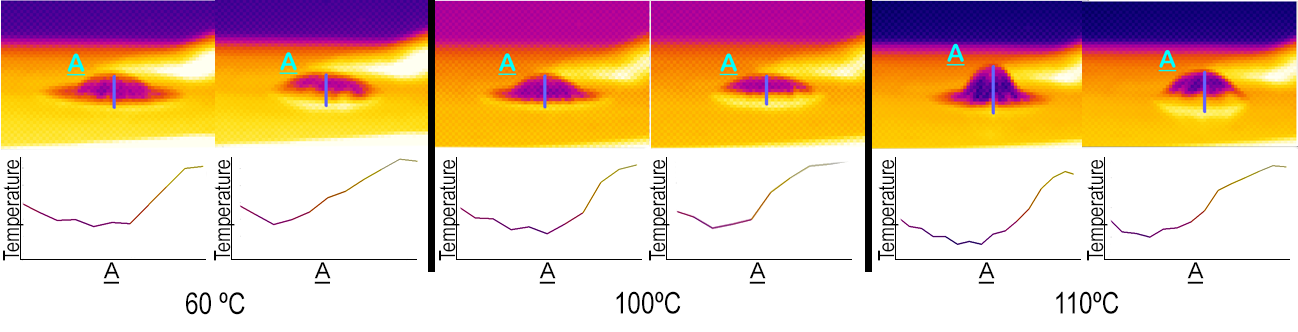
\includegraphics[width=1\linewidth]{Figures/5.Chapter/hexp.png}
\caption{Side view of the water droplets impacting the hydrophilic foil at 2 m/s: spreading and receding phases}
\label{fig:hexp}
\end{figure}

\begin{figure}[h]
\centering
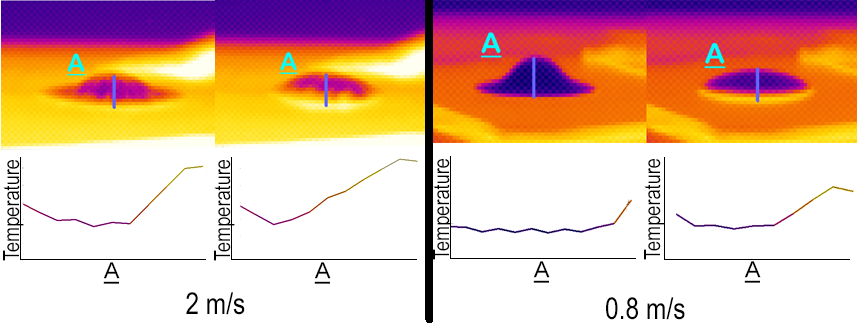
\includegraphics[width=0.66\linewidth]{Figures/5.Chapter/hexp2.png}
\caption{Side view Results for 60ºC during the spreading and receding phases}
\label{fig:hexp2}
\end{figure}

\section{Bottom View}

\par The images obtained in this configuration are mainly bidimensional temperature maps of the area on the surface corresponding to the area that is wetted by the droplet. From this map one can obtain the distribution of the temperature along the droplet radius for small time steps. Further post processing of the collected data was used to compute the heat flux and cooling effectiveness (as explained in Chapter 2), to compare the results obtained in the various experimental conditions. The connection between the high-speed images, temperature map and temperature plot is depicted Figure \ref{fig:hexp}.\\

\begin{figure}[h]
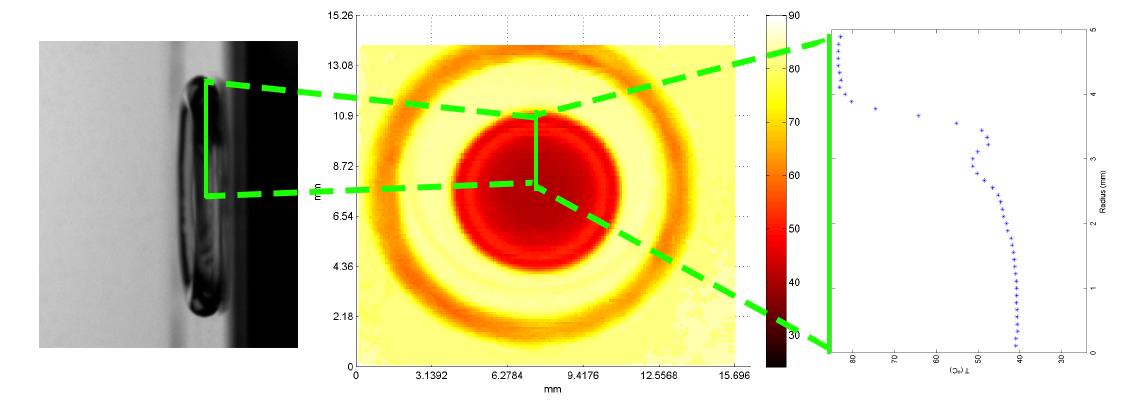
\includegraphics[width=1\linewidth]{Figures/5.Chapter/example.png}
\caption{Example of the results representation}
\label{fig:hexp}
\end{figure}

\par In fact various conditions were tested, namely two different impact velocities, 0.8 m/s and 2 m/s, and four initial foil temperature values, for conditions before and after the saturation point, 60ºC, 80ºC, 100ºC and 110ºC. Additionally, two different wettability conditions were compared, namely using the hydrophilic foil and the super-hydrophobic, coated foil. Finally, tests were also performed with two liquids: water and ethanol. As for each of the conditions, 5 different experiments were made, so that the repeatability of the tests could be confirmed. In Figure \ref{fig:repeat} the repeatability of these tests can be seen with the example of the 60ºC results for 2 m/s.\\

\begin{figure}[h]
\centering
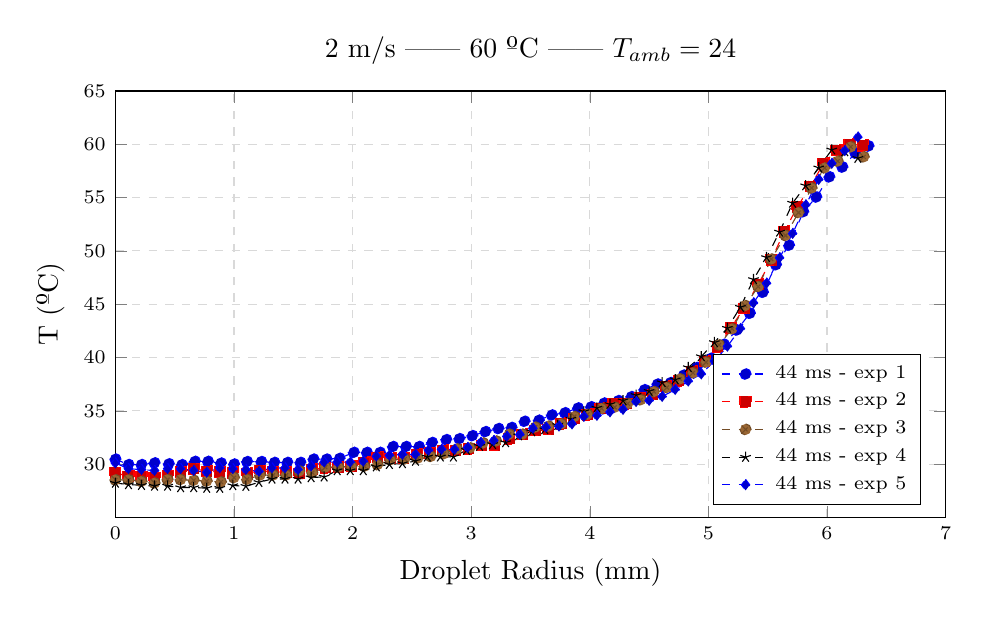
\begin{tikzpicture}
\begin{axis}[
	title = {2 m/s || 60 ºC || $T_{amb}=24$},
    tick label style={font=\scriptsize},
    legend style={font=\scriptsize,/tikz/column 2/.style={column sep=5pt},},
    %legend columns=2,
    legend cell align=left,
	legend pos =south east,
    grid=major, % Display a grid
    grid style={dashed,gray!30}, % Set the style
    xlabel={Droplet Radius (mm)},
    ylabel={T (ºC)}, 
    ymin = 25, ymax = 65,
    ytick={30,35,...,120},
    %yticklabels={300,325,350,375,400,425,450,475,500,525},
    xmin = 0, xmax = 7,
    %ytick={0,1600,...,11200},
    %yticklabel style={
    %    /pgf/number format/fixed,
    %    /pgf/number format/precision=5},
	%scaled y ticks=false,
    width=1\textwidth, 
    height=7cm,
    cycle list name= color
    ]
\addplot+[dashed]
coordinates {(	0	,	30.48	)
(	0.11	,	29.97	)
(	0.22	,	29.97	)
(	0.33	,	30.13	)
(	0.45	,	30.04	)
(	0.56	,	29.96	)
(	0.67	,	30.27	)
(	0.78	,	30.27	)
(	0.89	,	30.11	)
(	1	,	30.02	)
(	1.11	,	30.25	)
(	1.23	,	30.25	)
(	1.34	,	30.17	)
(	1.45	,	30.17	)
(	1.56	,	30.17	)
(	1.67	,	30.48	)
(	1.78	,	30.48	)
(	1.89	,	30.56	)
(	2.01	,	31.11	)
(	2.12	,	31.11	)
(	2.23	,	31.11	)
(	2.34	,	31.66	)
(	2.45	,	31.66	)
(	2.56	,	31.66	)
(	2.67	,	32.04	)
(	2.79	,	32.31	)
(	2.9	,	32.4	)
(	3.01	,	32.68	)
(	3.12	,	33.06	)
(	3.23	,	33.35	)
(	3.34	,	33.45	)
(	3.45	,	34.03	)
(	3.57	,	34.13	)
(	3.68	,	34.62	)
(	3.79	,	34.83	)
(	3.9	,	35.28	)
(	4.01	,	35.39	)
(	4.12	,	35.74	)
(	4.24	,	35.97	)
(	4.35	,	36.34	)
(	4.46	,	36.99	)
(	4.57	,	37.52	)
(	4.68	,	37.66	)
(	4.79	,	38.36	)
(	4.9	,	39.07	)
(	5.02	,	39.94	)
(	5.13	,	41.25	)
(	5.24	,	42.58	)
(	5.35	,	44.15	)
(	5.46	,	46.12	)
(	5.57	,	48.7	)
(	5.68	,	50.53	)
(	5.8	,	53.67	)
(	5.91	,	55.05	)
(	6.02	,	56.94	)
(	6.13	,	57.86	)
(	6.24	,	59.17	)
(	6.35	,	59.83	)
};
\addlegendentry{44 ms - exp 1}

\addplot+[dashed]
coordinates {(	0	,	29.18	)
(	0.11	,	28.88	)
(	0.22	,	28.81	)
(	0.33	,	28.73	)
(	0.44	,	28.9	)
(	0.55	,	29.28	)
(	0.66	,	29.58	)
(	0.77	,	29.36	)
(	0.88	,	29.29	)
(	0.99	,	29.22	)
(	1.11	,	29.15	)
(	1.22	,	29.38	)
(	1.33	,	29.31	)
(	1.44	,	29.24	)
(	1.55	,	29.17	)
(	1.66	,	29.53	)
(	1.77	,	29.66	)
(	1.88	,	29.73	)
(	1.99	,	29.8	)
(	2.1	,	30.16	)
(	2.21	,	30.66	)
(	2.32	,	30.58	)
(	2.43	,	30.58	)
(	2.54	,	30.93	)
(	2.65	,	31.08	)
(	2.76	,	31.31	)
(	2.87	,	31.31	)
(	2.98	,	31.47	)
(	3.09	,	31.78	)
(	3.2	,	31.78	)
(	3.32	,	32.39	)
(	3.43	,	32.83	)
(	3.54	,	33.18	)
(	3.65	,	33.27	)
(	3.76	,	33.82	)
(	3.87	,	34.28	)
(	3.98	,	34.67	)
(	4.09	,	35.24	)
(	4.2	,	35.67	)
(	4.31	,	35.67	)
(	4.42	,	36.22	)
(	4.53	,	36.57	)
(	4.64	,	37.31	)
(	4.75	,	37.81	)
(	4.86	,	38.72	)
(	4.97	,	39.67	)
(	5.08	,	41.03	)
(	5.19	,	42.81	)
(	5.3	,	44.63	)
(	5.42	,	46.87	)
(	5.53	,	49.15	)
(	5.64	,	51.83	)
(	5.75	,	54.13	)
(	5.86	,	56.06	)
(	5.97	,	58.19	)
(	6.08	,	59.43	)
(	6.19	,	60.02	)
(	6.3	,	59.89	)
};
\addlegendentry{44 ms - exp 2}

\addplot+[dashed]
coordinates {(	0	,	28.54	)
(	0.11	,	28.54	)
(	0.22	,	28.39	)
(	0.33	,	28.24	)
(	0.44	,	28.56	)
(	0.55	,	28.56	)
(	0.66	,	28.49	)
(	0.77	,	28.42	)
(	0.89	,	28.34	)
(	1	,	28.74	)
(	1.11	,	28.59	)
(	1.22	,	28.98	)
(	1.33	,	28.98	)
(	1.44	,	28.98	)
(	1.55	,	29.36	)
(	1.66	,	29.21	)
(	1.77	,	29.73	)
(	1.88	,	29.73	)
(	1.99	,	29.81	)
(	2.1	,	29.81	)
(	2.21	,	29.96	)
(	2.32	,	30.41	)
(	2.44	,	30.49	)
(	2.55	,	30.57	)
(	2.66	,	30.73	)
(	2.77	,	30.98	)
(	2.88	,	31.44	)
(	2.99	,	31.53	)
(	3.1	,	31.99	)
(	3.21	,	32.17	)
(	3.32	,	32.82	)
(	3.43	,	32.82	)
(	3.54	,	33.48	)
(	3.65	,	33.58	)
(	3.76	,	33.78	)
(	3.87	,	34.47	)
(	3.98	,	34.68	)
(	4.1	,	35.23	)
(	4.21	,	35.34	)
(	4.32	,	35.69	)
(	4.43	,	36.04	)
(	4.54	,	36.81	)
(	4.65	,	37.2	)
(	4.76	,	38	)
(	4.87	,	38.57	)
(	4.98	,	39.57	)
(	5.09	,	41.19	)
(	5.2	,	42.7	)
(	5.31	,	44.87	)
(	5.42	,	46.66	)
(	5.53	,	49.24	)
(	5.65	,	51.45	)
(	5.76	,	53.6	)
(	5.87	,	55.9	)
(	5.98	,	57.78	)
(	6.09	,	58.42	)
(	6.2	,	59.75	)
(	6.31	,	58.82	)
};
\addlegendentry{44 ms - exp 3}

\addplot+[dashed]
coordinates {(	0	,	28.24	)
(	0.11	,	28.1	)
(	0.22	,	28.03	)
(	0.33	,	27.96	)
(	0.44	,	27.96	)
(	0.55	,	27.82	)
(	0.66	,	27.82	)
(	0.77	,	27.76	)
(	0.88	,	27.76	)
(	0.99	,	28.01	)
(	1.1	,	27.94	)
(	1.21	,	28.31	)
(	1.32	,	28.62	)
(	1.43	,	28.62	)
(	1.54	,	28.62	)
(	1.65	,	28.75	)
(	1.76	,	28.82	)
(	1.87	,	29.41	)
(	1.98	,	29.41	)
(	2.09	,	29.41	)
(	2.2	,	29.77	)
(	2.31	,	29.99	)
(	2.42	,	30.07	)
(	2.53	,	30.3	)
(	2.63	,	30.69	)
(	2.74	,	30.69	)
(	2.85	,	30.69	)
(	2.96	,	31.32	)
(	3.07	,	31.69	)
(	3.18	,	31.86	)
(	3.29	,	32.04	)
(	3.4	,	32.68	)
(	3.51	,	33.06	)
(	3.62	,	33.25	)
(	3.73	,	33.65	)
(	3.84	,	34.24	)
(	3.95	,	34.94	)
(	4.06	,	35.28	)
(	4.17	,	35.62	)
(	4.28	,	35.97	)
(	4.39	,	36.47	)
(	4.5	,	36.85	)
(	4.61	,	37.66	)
(	4.72	,	37.93	)
(	4.83	,	39.07	)
(	4.94	,	40.1	)
(	5.05	,	41.42	)
(	5.16	,	42.76	)
(	5.27	,	44.73	)
(	5.38	,	47.33	)
(	5.49	,	49.39	)
(	5.6	,	51.78	)
(	5.71	,	54.49	)
(	5.82	,	56.12	)
(	5.93	,	57.8	)
(	6.04	,	59.48	)
(	6.15	,	59.31	)
(	6.26	,	58.69	)
};
\addlegendentry{44 ms - exp 4}

\addplot+[dashed]
coordinates {(	0	,	30.11	)
(	0.11	,	29.58	)
(	0.22	,	29.5	)
(	0.33	,	29.41	)
(	0.44	,	29.58	)
(	0.55	,	29.58	)
(	0.66	,	29.41	)
(	0.77	,	29.24	)
(	0.88	,	29.66	)
(	0.99	,	29.57	)
(	1.1	,	29.49	)
(	1.21	,	29.33	)
(	1.32	,	29.65	)
(	1.43	,	29.65	)
(	1.54	,	29.49	)
(	1.65	,	29.81	)
(	1.76	,	30.2	)
(	1.87	,	30.2	)
(	1.98	,	30.2	)
(	2.09	,	30.28	)
(	2.2	,	30.75	)
(	2.31	,	30.84	)
(	2.42	,	30.92	)
(	2.53	,	30.92	)
(	2.64	,	31.31	)
(	2.75	,	31.39	)
(	2.86	,	31.39	)
(	2.97	,	31.57	)
(	3.08	,	32.04	)
(	3.19	,	32.22	)
(	3.3	,	32.61	)
(	3.41	,	32.79	)
(	3.52	,	33.37	)
(	3.63	,	33.47	)
(	3.74	,	33.57	)
(	3.85	,	33.77	)
(	3.95	,	34.47	)
(	4.06	,	34.57	)
(	4.17	,	34.9	)
(	4.28	,	35.13	)
(	4.39	,	35.87	)
(	4.5	,	35.98	)
(	4.61	,	36.35	)
(	4.72	,	37	)
(	4.83	,	37.79	)
(	4.94	,	38.46	)
(	5.05	,	39.67	)
(	5.16	,	41.06	)
(	5.27	,	42.71	)
(	5.38	,	45.12	)
(	5.49	,	46.97	)
(	5.6	,	49.35	)
(	5.71	,	51.63	)
(	5.82	,	54.3	)
(	5.93	,	56.69	)
(	6.04	,	58.2	)
(	6.15	,	59.39	)
(	6.26	,	60.66	)
};
\addlegendentry{44 ms - exp 5}
\end{axis}
\end{tikzpicture}
\caption{Repeatability of the experiments}
\label{fig:repeat}
\end{figure}

\subsection{Result of applying the custom made calibration method}

\par Some preliminary images were taken using the camera calibration, which were then compared to those using the custom made calibration detailed in Chapter 4. To evaluate the quality of the calibration it is important to compare the results and interpret the differences.  The result of applying the calibration process is discussed for the impact of water droplets at 2 m/s and 0.8 m/s, for initial foil temperatures of 60ºC, 100ºC and 110ºC. Due to deviations in the ADU to Celsius conversion, these exact temperature values could not always be achieved, so the real working temperature is provided. Figure \ref{fig:calibcomp2} compares the temperature variation on the foil as a function of the spreading droplet radius for the impact velocity of 0.8 m/s the different curves in each plot correspond to different time instants of the spreading. So, in the time instants chosen to depict impact (e.g. t=1ms) the temperature decrease of the center region of the droplet is small and swiftly recovers for the still small spreading ratio. This contrasts in the higher temperature drops at later time instants.\\

\par Before comparing the images, one should bare in mind the differences in their conditions. The results before calibration were taken at a different ambient temperature, proximity to the droplet and framerate. The average framerate of the results before the calibration is 990 fps, and 1100 after. These improvements were the result of having more experience dealing with the camera during this work. This results in better temporal and spatial resolution in the data obtained after the calibration. Hence one can only compare similar frames and differences may be accentuated by that. \\

\par One important aspect is that the apparent diameter (the diamenter that one can perceive from the temperature plots, that is representative of the wetted area) is approximately the same with and without this improved calibration process. During the spreading phase (all the points before 13 ms) the new calibration and method captures a bit of the air trapping effect mentioned previously in Section \ref{sec:heat}. The mentioned effect is not captured in the results without the calibration. Another thing that was corrected, was the fact that the temperature at the center of the droplet (r=0) would drop bellow the ambient temperature in the Figure \ref{fig:calibcomp2}. This is impossible because the droplet is at ambient temperature. The cause of this is related to optical effects, that were nullified by the calibration. On the other hand the results obtained using the custom made calibration have some noise that couldn't be addressed without losing resolution. The cause of the noise is probably the improved setup that allowed higher spatial resolution. So while there are advantages using the factory calibration, the proposed calibration can better portrait the physical phenomena. \\

\begin{figure}
\centering
\subfigure[Before custom calibration]{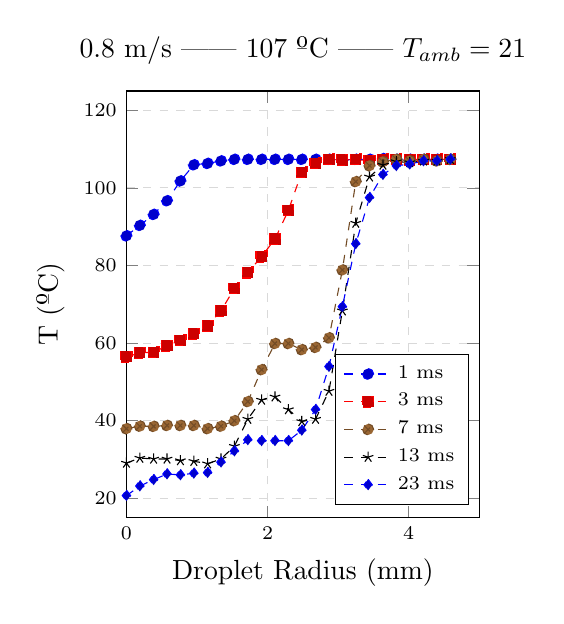
\begin{tikzpicture}
\begin{axis}[
	title = {0.8 m/s || 107 ºC || $T_{amb}=21$},
    tick label style={font=\scriptsize},
    legend style={font=\scriptsize,/tikz/column 2/.style={column sep=5pt},},
    %legend columns=2,
    legend cell align=left,
	legend pos =south east,
    grid=major, % Display a grid
    grid style={dashed,gray!30}, % Set the style
    xlabel={Droplet Radius (mm)},
    ylabel={T (ºC)}, 
    ymin = 15, ymax = 125,
    ytick={20,40,...,120},
    %yticklabels={300,325,350,375,400,425,450,475,500,525},
    xmin = 0, xmax = 5,
    %ytick={0,1600,...,11200},
    %yticklabel style={
    %    /pgf/number format/fixed,
    %    /pgf/number format/precision=5},
	%scaled y ticks=false,
    width=0.5\textwidth, 
    height=7cm,
    cycle list name= color
    ]
\addplot+[dashed]
coordinates {(	0	,	87.65	)
(	0.19	,	90.34	)
(	0.385	,	93.17	)
(	0.575	,	96.69	)
(	0.765	,	101.8	)
(	0.955	,	105.96	)
(	1.15	,	106.32	)
(	1.34	,	106.96	)
(	1.53	,	107.37	)
(	1.72	,	107.37	)
(	1.915	,	107.37	)
(	2.105	,	107.37	)
(	2.295	,	107.37	)
(	2.485	,	107.37	)
(	2.68	,	107.37	)
(	2.87	,	107.37	)
(	3.06	,	107.19	)
(	3.25	,	107.37	)
(	3.445	,	107.37	)
(	3.635	,	107.55	)
(	3.825	,	107.37	)
(	4.015	,	107.37	)
(	4.21	,	107.37	)
(	4.4	,	107.37	)
(	4.59	,	107.37	)
};
\addlegendentry{1 ms}

\addplot+[dashed]
coordinates {(	0	,	56.42	)
(	0.19	,	57.47	)
(	0.385	,	57.65	)
(	0.575	,	59.29	)
(	0.765	,	60.71	)
(	0.955	,	62.4	)
(	1.15	,	64.4	)
(	1.34	,	68.33	)
(	1.53	,	74.09	)
(	1.72	,	78.19	)
(	1.915	,	82.3	)
(	2.105	,	86.82	)
(	2.295	,	94.22	)
(	2.485	,	104.08	)
(	2.68	,	106.32	)
(	2.87	,	107.37	)
(	3.06	,	107.19	)
(	3.25	,	107.37	)
(	3.445	,	106.96	)
(	3.635	,	107.37	)
(	3.825	,	107.37	)
(	4.015	,	107.19	)
(	4.21	,	107.37	)
(	4.4	,	107.37	)
(	4.59	,	107.37	)
};
\addlegendentry{3 ms}

\addplot+[dashed]
coordinates {(	0	,	37.93	)
(	0.19	,	38.57	)
(	0.385	,	38.52	)
(	0.575	,	38.75	)
(	0.765	,	38.75	)
(	0.955	,	38.75	)
(	1.15	,	37.93	)
(	1.34	,	38.57	)
(	1.53	,	39.98	)
(	1.72	,	44.91	)
(	1.915	,	53.13	)
(	2.105	,	59.88	)
(	2.295	,	59.88	)
(	2.485	,	58.29	)
(	2.68	,	58.88	)
(	2.87	,	61.35	)
(	3.06	,	78.84	)
(	3.25	,	101.62	)
(	3.445	,	105.72	)
(	3.635	,	106.73	)
(	3.825	,	107.37	)
(	4.015	,	106.96	)
(	4.21	,	107.37	)
(	4.4	,	106.96	)
(	4.59	,	107.37	)
};
\addlegendentry{7 ms}

\addplot+[dashed]
coordinates {(	0	,	29.07	)
(	0.19	,	30.35	)
(	0.385	,	30.12	)
(	0.575	,	30.12	)
(	0.765	,	29.71	)
(	0.955	,	29.53	)
(	1.15	,	28.89	)
(	1.34	,	30.12	)
(	1.53	,	33.41	)
(	1.72	,	40.39	)
(	1.915	,	45.32	)
(	2.105	,	46.14	)
(	2.295	,	42.86	)
(	2.485	,	39.8	)
(	2.68	,	40.39	)
(	2.87	,	47.61	)
(	3.06	,	68.33	)
(	3.25	,	90.93	)
(	3.445	,	102.85	)
(	3.635	,	105.9	)
(	3.825	,	106.78	)
(	4.015	,	106.55	)
(	4.21	,	106.96	)
(	4.4	,	106.96	)
(	4.59	,	107.37	)
};
\addlegendentry{13 ms}

\addplot+[dashed]
coordinates {(	0	,	20.67	)
(	0.19	,	23.13	)
(	0.385	,	24.78	)
(	0.575	,	26.24	)
(	0.765	,	26.01	)
(	0.955	,	26.42	)
(	1.15	,	26.6	)
(	1.34	,	29.3	)
(	1.53	,	32.17	)
(	1.72	,	35.05	)
(	1.915	,	34.82	)
(	2.105	,	34.82	)
(	2.295	,	34.82	)
(	2.485	,	37.52	)
(	2.68	,	42.86	)
(	2.87	,	53.95	)
(	3.06	,	69.39	)
(	3.25	,	85.59	)
(	3.445	,	97.51	)
(	3.635	,	103.44	)
(	3.825	,	105.72	)
(	4.015	,	106.14	)
(	4.21	,	106.96	)
(	4.4	,	106.96	)
(	4.59	,	107.37	)
};
\addlegendentry{23 ms}
\end{axis}
\end{tikzpicture}}
\subfigure[After custom calibration]{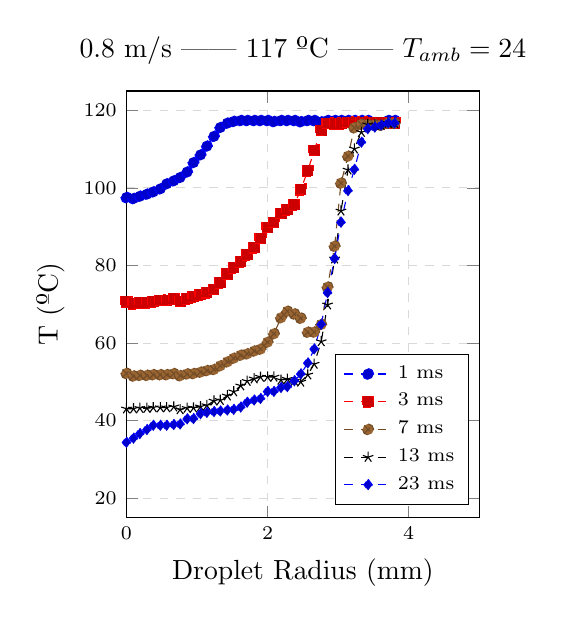
\begin{tikzpicture}
\begin{axis}[
	title = {0.8 m/s || 117 ºC || $T_{amb}=24$},
    tick label style={font=\scriptsize},
    legend style={font=\scriptsize,/tikz/column 2/.style={column sep=5pt},},
    %legend columns=2,
    legend cell align=left,
	legend pos =south east,
    grid=major, % Display a grid
    grid style={dashed,gray!30}, % Set the style
    xlabel={Droplet Radius (mm)},
    ylabel={T (ºC)}, 
    ymin = 15, ymax = 125,
    ytick={20,40,...,120},
    %yticklabels={300,325,350,375,400,425,450,475,500,525},
    xmin = 0, xmax = 5,
    %ytick={0,1600,...,11200},
    %yticklabel style={
    %    /pgf/number format/fixed,
    %    /pgf/number format/precision=5},
	%scaled y ticks=false,
    width=0.5\textwidth, height=7cm,
    cycle list name= color
    ]
\addplot+[dashed]
coordinates {(	0	,	97.52	)
(	0.1	,	97.26	)
(	0.19	,	97.85	)
(	0.29	,	98.38	)
(	0.38	,	98.98	)
(	0.48	,	99.76	)
(	0.57	,	101.05	)
(	0.67	,	101.82	)
(	0.76	,	102.68	)
(	0.86	,	104.1	)
(	0.95	,	106.53	)
(	1.05	,	108.52	)
(	1.14	,	110.77	)
(	1.24	,	113.29	)
(	1.33	,	115.57	)
(	1.43	,	116.69	)
(	1.52	,	117.14	)
(	1.62	,	117.37	)
(	1.71	,	117.37	)
(	1.81	,	117.37	)
(	1.9	,	117.37	)
(	2	,	117.37	)
(	2.09	,	117.1	)
(	2.19	,	117.37	)
(	2.28	,	117.37	)
(	2.38	,	117.37	)
(	2.47	,	117.06	)
(	2.57	,	117.37	)
(	2.66	,	117.37	)
(	2.76	,	117.02	)
(	2.85	,	117.37	)
(	2.95	,	117.37	)
(	3.04	,	117.37	)
(	3.14	,	117.37	)
(	3.23	,	117.37	)
(	3.33	,	117.37	)
(	3.42	,	117.37	)
(	3.52	,	116.8	)
(	3.61	,	116.76	)
(	3.71	,	117.37	)
(	3.8	,	117.37	)
};
\addlegendentry{1 ms}

\addplot+[dashed]
coordinates {(	0	,	70.61	)
(	0.1	,	70.16	)
(	0.19	,	70.4	)
(	0.29	,	70.4	)
(	0.38	,	70.63	)
(	0.48	,	71.08	)
(	0.57	,	71.08	)
(	0.67	,	71.45	)
(	0.76	,	70.78	)
(	0.86	,	71.41	)
(	0.95	,	71.99	)
(	1.05	,	72.51	)
(	1.14	,	73.05	)
(	1.24	,	73.92	)
(	1.33	,	75.58	)
(	1.43	,	77.81	)
(	1.52	,	79.42	)
(	1.62	,	80.97	)
(	1.71	,	82.76	)
(	1.81	,	84.66	)
(	1.9	,	87.07	)
(	2	,	89.89	)
(	2.09	,	91.11	)
(	2.19	,	93.47	)
(	2.28	,	94.33	)
(	2.38	,	95.68	)
(	2.47	,	99.61	)
(	2.57	,	104.39	)
(	2.66	,	109.67	)
(	2.76	,	114.9	)
(	2.85	,	116.64	)
(	2.95	,	116.6	)
(	3.04	,	116.54	)
(	3.14	,	116.94	)
(	3.23	,	116.91	)
(	3.33	,	116.88	)
(	3.42	,	116.84	)
(	3.52	,	116.8	)
(	3.61	,	116.76	)
(	3.71	,	116.7	)
(	3.8	,	116.65	)
};
\addlegendentry{3 ms}

\addplot+[dashed]
coordinates {(	0	,	52.18	)
(	0.1	,	51.5	)
(	0.19	,	51.67	)
(	0.29	,	51.67	)
(	0.38	,	51.84	)
(	0.48	,	51.84	)
(	0.57	,	51.84	)
(	0.67	,	52.11	)
(	0.76	,	51.58	)
(	0.86	,	52.04	)
(	0.95	,	52.13	)
(	1.05	,	52.5	)
(	1.14	,	52.89	)
(	1.24	,	53.19	)
(	1.33	,	54.12	)
(	1.43	,	55.15	)
(	1.52	,	56.08	)
(	1.62	,	56.86	)
(	1.71	,	57.21	)
(	1.81	,	57.93	)
(	1.9	,	58.43	)
(	2	,	60.23	)
(	2.09	,	62.39	)
(	2.19	,	66.52	)
(	2.28	,	68.19	)
(	2.38	,	67.5	)
(	2.47	,	66.4	)
(	2.57	,	62.8	)
(	2.66	,	62.84	)
(	2.76	,	64.79	)
(	2.85	,	74.42	)
(	2.95	,	84.98	)
(	3.04	,	101.24	)
(	3.14	,	108.17	)
(	3.23	,	115.5	)
(	3.33	,	116.38	)
(	3.42	,	116.3	)
(	3.52	,	116.22	)
(	3.61	,	116.14	)
(	3.71	,	116.7	)
(	3.8	,	116.65	)
};
\addlegendentry{7 ms}

\addplot+[dashed]
coordinates {(	0	,	43.06	)
(	0.1	,	43.06	)
(	0.19	,	43.2	)
(	0.29	,	43.2	)
(	0.38	,	43.35	)
(	0.48	,	43.35	)
(	0.57	,	43.35	)
(	0.67	,	43.57	)
(	0.76	,	42.84	)
(	0.86	,	43.21	)
(	0.95	,	43.29	)
(	1.05	,	43.6	)
(	1.14	,	43.92	)
(	1.24	,	45.08	)
(	1.33	,	45.25	)
(	1.43	,	46.41	)
(	1.52	,	47.47	)
(	1.62	,	49	)
(	1.71	,	50.17	)
(	1.81	,	50.8	)
(	1.9	,	51.24	)
(	2	,	51.26	)
(	2.09	,	51.26	)
(	2.19	,	50.46	)
(	2.28	,	50.71	)
(	2.38	,	50.22	)
(	2.47	,	49.97	)
(	2.57	,	51.82	)
(	2.66	,	54.59	)
(	2.76	,	60.39	)
(	2.85	,	69.88	)
(	2.95	,	81.73	)
(	3.04	,	94.08	)
(	3.14	,	104.64	)
(	3.23	,	110.08	)
(	3.33	,	114.35	)
(	3.42	,	116.3	)
(	3.52	,	116.22	)
(	3.61	,	116.14	)
(	3.71	,	116.7	)
(	3.8	,	116.65	)
};
\addlegendentry{13 ms}

\addplot+[dashed]
coordinates {(	0	,	34.36	)
(	0.1	,	35.44	)
(	0.19	,	36.61	)
(	0.29	,	37.63	)
(	0.38	,	38.75	)
(	0.48	,	38.75	)
(	0.57	,	38.75	)
(	0.67	,	38.95	)
(	0.76	,	39.08	)
(	0.86	,	40.41	)
(	0.95	,	40.48	)
(	1.05	,	41.74	)
(	1.14	,	42.05	)
(	1.24	,	42.28	)
(	1.33	,	42.44	)
(	1.43	,	42.69	)
(	1.52	,	42.85	)
(	1.62	,	43.45	)
(	1.71	,	44.7	)
(	1.81	,	45.27	)
(	1.9	,	45.66	)
(	2	,	47.48	)
(	2.09	,	47.48	)
(	2.19	,	48.49	)
(	2.28	,	48.72	)
(	2.38	,	50.22	)
(	2.47	,	52	)
(	2.57	,	54.82	)
(	2.66	,	58.44	)
(	2.76	,	64.79	)
(	2.85	,	72.95	)
(	2.95	,	81.73	)
(	3.04	,	91.1	)
(	3.14	,	99.25	)
(	3.23	,	104.75	)
(	3.33	,	111.74	)
(	3.42	,	115.21	)
(	3.52	,	115.63	)
(	3.61	,	116.14	)
(	3.71	,	116.7	)
(	3.8	,	116.65	)
};
\addlegendentry{23 ms}
\end{axis}
\end{tikzpicture}}
\caption{Comparison between results with and without the proposed calibration}
\label{fig:calibcomp2}
\end{figure}

\subsection{Simultaneous analysis of droplet dynamics and thermal processes}

\begin{figure}
\centering
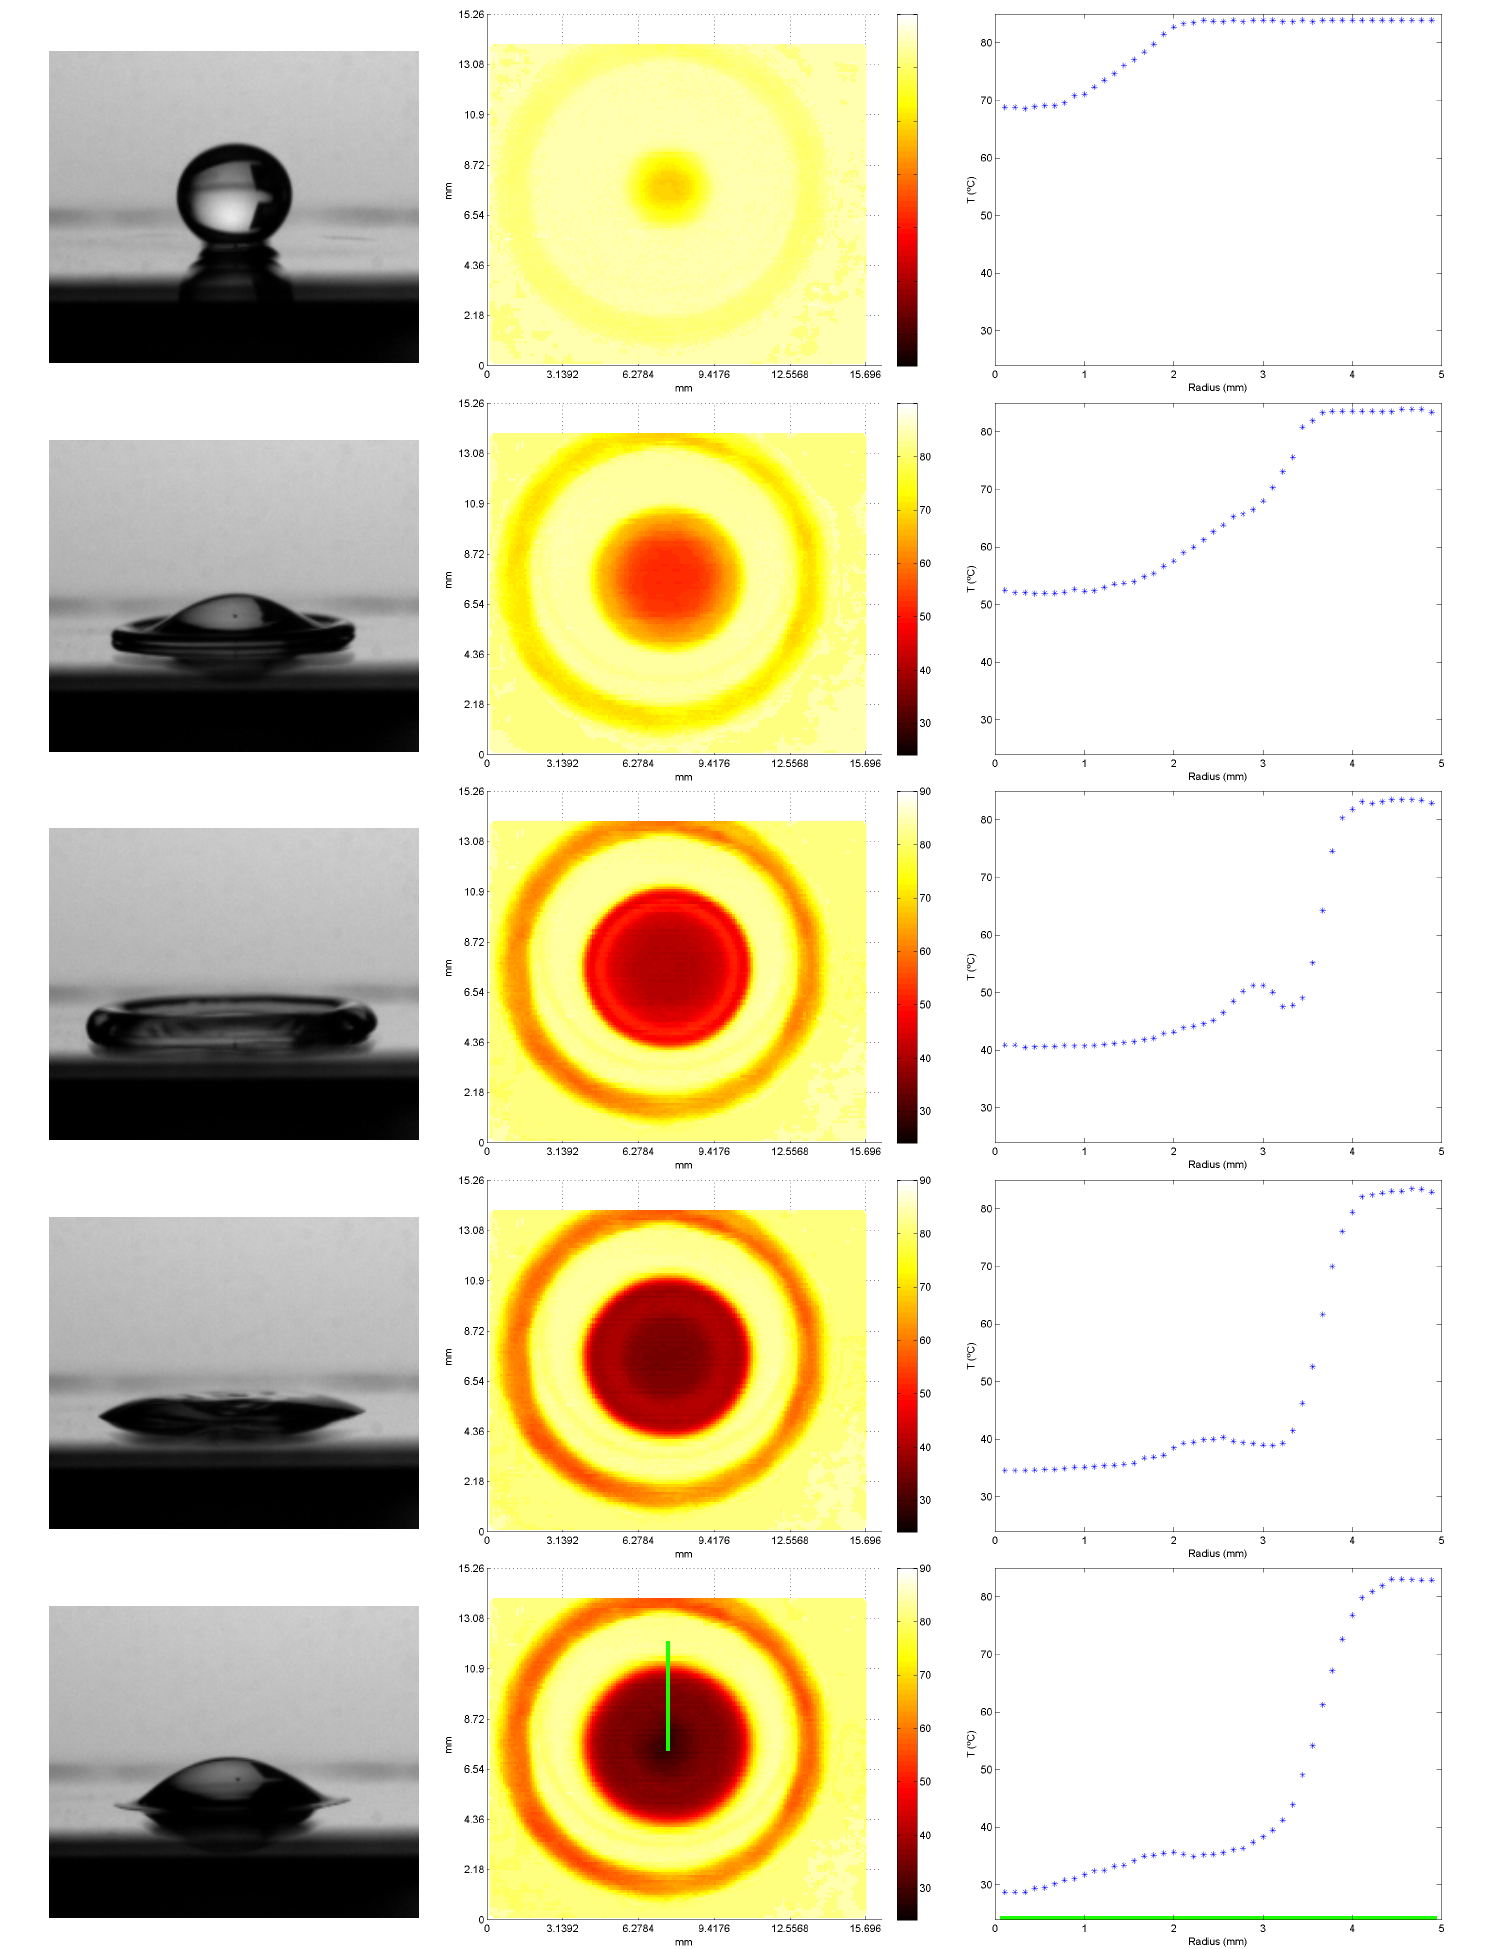
\includegraphics[width=1\linewidth]{Figures/5.Chapter/IRvsHR.png}
\caption{Comparison between High Speed camera images and Infra Red images for 0.8m/s and 80ºC at 0, 2, 6, 12 and 22 ms after the first contact on a hydrophilic surface}
\label{fig:irvshr}
\end{figure}

\par One of the main objectives of this work is to use the high-speed camera simultaneously with the IR Camera to compare physical phenomena with thermal phenomena. The results were put together in Figure \ref{fig:irvshr}. In this figure it is possible to see some of the stages of a droplet impact. Analyzing the images, it's observable the physical phenomena that have an impact on heat transfer. During the spreading, the lamella's rim is visible in the temperature maps, as introduced in Section \ref{sec:heat}, starts forming in the second millisecond. When the edge reaches maximum diameter it reverses direction and starts the recoiling phase, shown in the 12 ms images. The thickness of the water layer is smaller right before the lamella's edge. In this area there is less heat removal. So, as expected, one can see a ring of higher temperatures, and a slope in the plot. After the recoiling phase the droplet starts to stabilize, and due to it's hemispherical shape the heat flux is higher at the center, so the temperature is lower in the center. Although here there is no rim in the lamella by this phase, one can clearly see the lighter ring on the IR Image. This is the cause of thermal inertia.

\par Another type of results can be obtained for the collected data and these are the heat flux and cooling effectiveness. Starting with the heat flux, an example of the obtained graphic can be seen in Figure \ref{fig:fluex}. Looking at the heat flux, one can see the expected phenomena, described in the literature \cite{pasandideh2001cooling}. There are only some comparable results between Figure \ref{fig:fluxo} and the collected results, as the timestep of the simulation is much smaller. The contact edge heat flux peak couldn't be captured in the initial timesteps, but is clear in the posterior frames. This contact edge peak is a reflection of cold water being pushed to the edge of the lamella as the droplet spreads. In the center the spatial gradient is ignored because of the problem's axisymmetry. The highest peaks for the initial times aren't captured by the IR Camera, but the flux drop before the peak, in Figure \ref{fig:fluxo}, is visible in the 1ms and 2ms frame. The spatial dispersion of the flux in early frames is clear in the experimental results. This may be caused by thermal inertia and heat diffusion along the foil. This may also be the cause for the innexistence of a peak in the early frames. In the last frame, which, according to Figure \ref{fig:diameter}, is already during the receding phase, the heat flux is negative after the droplet edge. This is caused by the area being no longer wetted and is now heating again. Also the heat flux drop before the contact angle peak is an indicative of the presence of the lamella's rim in that area. Also the heat flux is very small compared to other timesteps due to the droplet temperature raise.\\


\begin{figure}[h!]
\centering
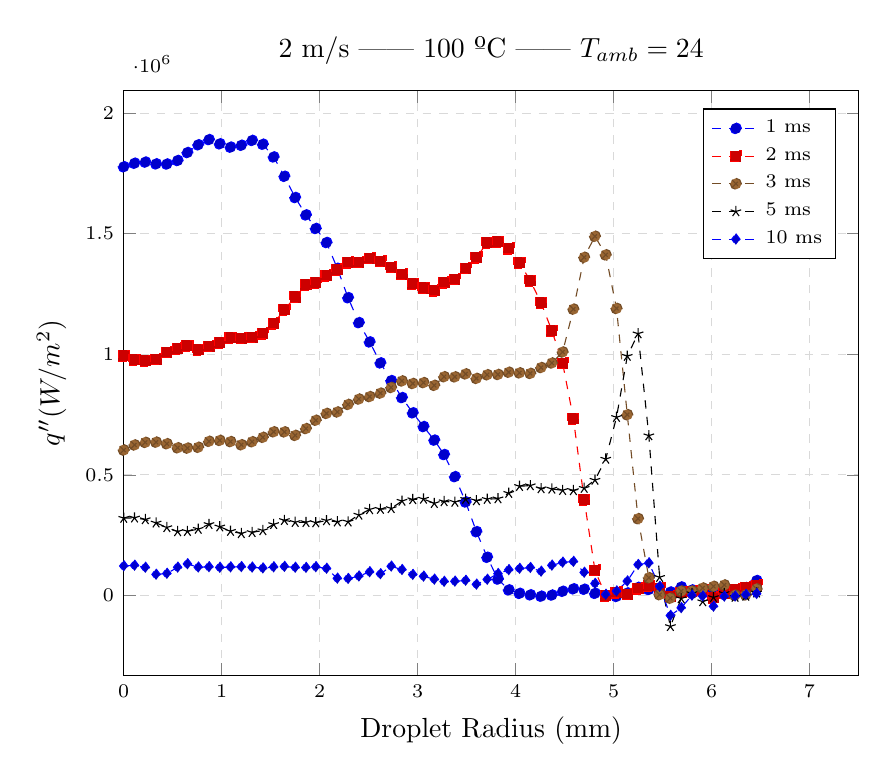
\begin{tikzpicture}
\begin{axis}[
	title = {2 m/s || 100 ºC || $T_{amb}=24$},
    tick label style={font=\scriptsize},
    legend style={font=\scriptsize,/tikz/column 2/.style={column sep=5pt},},
    %legend columns=2,
    legend cell align=left,
	legend pos =north east,
    grid=major, % Display a grid
    grid style={dashed,gray!30}, % Set the style
    xlabel={Droplet Radius (mm)},
    ylabel={$q''(W/m^2)$}, 
    %ymin = 15, ymax = 125,
    %ytick={20,40,...,120},
    %yticklabels={300,325,350,375,400,425,450,475,500,525},
    xmin = 0, xmax = 7.5,
    %ytick={0,1600,...,11200},
    %yticklabel style={
    %    /pgf/number format/fixed,
    %    /pgf/number format/precision=5},
	%scaled y ticks=false,
    width=0.9\textwidth, 
    height=9cm,
    cycle list name= color
    ]
\addplot+[dashed]
coordinates {(	0	,	1777670.079	)
(	0.11	,	1792323.198	)
(	0.22	,	1797061.305	)
(	0.33	,	1789569.185	)
(	0.44	,	1789015.722	)
(	0.55	,	1803622.248	)
(	0.65	,	1836659.277	)
(	0.76	,	1868745.749	)
(	0.87	,	1890207.195	)
(	0.98	,	1872770.186	)
(	1.09	,	1858985.806	)
(	1.2	,	1866796.219	)
(	1.31	,	1886797.855	)
(	1.42	,	1871035.553	)
(	1.53	,	1818458.79	)
(	1.64	,	1738103.547	)
(	1.75	,	1650076.058	)
(	1.86	,	1578011.828	)
(	1.96	,	1521786.363	)
(	2.07	,	1463673.962	)
(	2.18	,	1356450.868	)
(	2.29	,	1234687.338	)
(	2.4	,	1131209.047	)
(	2.51	,	1051299.604	)
(	2.62	,	964361.1129	)
(	2.73	,	890905.7486	)
(	2.84	,	820486.8888	)
(	2.95	,	757411.9607	)
(	3.06	,	700437.3131	)
(	3.17	,	644241.2043	)
(	3.27	,	584413.7383	)
(	3.38	,	492724.449	)
(	3.49	,	387796.4609	)
(	3.6	,	264656.6861	)
(	3.71	,	158383.9646	)
(	3.82	,	68032.80929	)
(	3.93	,	23332.98041	)
(	4.04	,	8824.872215	)
(	4.15	,	2783.827432	)
(	4.26	,	-2946.812742	)
(	4.37	,	1783.017459	)
(	4.48	,	17428.61908	)
(	4.59	,	27766.9984	)
(	4.7	,	25929.14618	)
(	4.81	,	8913.264039	)
(	4.92	,	-461.1725983	)
(	5.03	,	-3885.427042	)
(	5.14	,	10510.44467	)
(	5.25	,	33569.04446	)
(	5.36	,	24609.65614	)
(	5.47	,	6504.078318	)
(	5.58	,	14471.4661	)
(	5.69	,	35286.16241	)
(	5.8	,	22937.69419	)
(	5.91	,	16717.33533	)
(	6.02	,	19095.65158	)
(	6.13	,	26500.66468	)
(	6.24	,	17516.80911	)
(	6.35	,	32445.82136	)
(	6.46	,	62028.02361	)
};
\addlegendentry{1 ms}

\addplot+[dashed]
coordinates {(	0	,	994416.6114	)
(	0.11	,	977868.5786	)
(	0.22	,	972484.0558	)
(	0.33	,	979964.5653	)
(	0.44	,	1009224.339	)
(	0.55	,	1024051.643	)
(	0.65	,	1035507.694	)
(	0.76	,	1018875.215	)
(	0.87	,	1033036.687	)
(	0.98	,	1047901.012	)
(	1.09	,	1067866.738	)
(	1.2	,	1066642.971	)
(	1.31	,	1070797.553	)
(	1.42	,	1086486.604	)
(	1.53	,	1127965.656	)
(	1.64	,	1185262.461	)
(	1.75	,	1237552.837	)
(	1.86	,	1287648.943	)
(	1.96	,	1296848.547	)
(	2.07	,	1326923.578	)
(	2.18	,	1351476.86	)
(	2.29	,	1380984.107	)
(	2.4	,	1382032.351	)
(	2.51	,	1399104.992	)
(	2.62	,	1386742.3	)
(	2.73	,	1361384.005	)
(	2.84	,	1332532.503	)
(	2.95	,	1291867.248	)
(	3.06	,	1275120.227	)
(	3.17	,	1264695.521	)
(	3.27	,	1297790.475	)
(	3.38	,	1310759.548	)
(	3.49	,	1357356.743	)
(	3.6	,	1401558.802	)
(	3.71	,	1462662.38	)
(	3.82	,	1466663.884	)
(	3.93	,	1439063.016	)
(	4.04	,	1380067.453	)
(	4.15	,	1304513.447	)
(	4.26	,	1213606.763	)
(	4.37	,	1097774.749	)
(	4.48	,	963623.8334	)
(	4.59	,	732954.8917	)
(	4.7	,	396736.0879	)
(	4.81	,	104345.5448	)
(	4.92	,	-870.3142338	)
(	5.03	,	12710.59066	)
(	5.14	,	5768.502396	)
(	5.25	,	29015.00339	)
(	5.36	,	40107.34728	)
(	5.47	,	29735.44666	)
(	5.58	,	-3364.906372	)
(	5.69	,	13370.9096	)
(	5.8	,	17872.4023	)
(	5.91	,	22126.82747	)
(	6.02	,	-8408.393299	)
(	6.13	,	10462.99961	)
(	6.24	,	25645.7798	)
(	6.35	,	34831.77943	)
(	6.46	,	42268.81389	)
};
\addlegendentry{2 ms}

\addplot+[dashed]
coordinates {(	0	,	603064.3463	)
(	0.11	,	624155.5002	)
(	0.22	,	634775.6785	)
(	0.33	,	635817.91	)
(	0.44	,	629201.713	)
(	0.55	,	612380.4361	)
(	0.65	,	611141.2904	)
(	0.76	,	614518.6137	)
(	0.87	,	639263.8912	)
(	0.98	,	643016.4578	)
(	1.09	,	638055.9843	)
(	1.2	,	625042.0919	)
(	1.31	,	637498.6336	)
(	1.42	,	655804.2419	)
(	1.53	,	678635.2239	)
(	1.64	,	678356.8117	)
(	1.75	,	663833.9141	)
(	1.86	,	692052.9325	)
(	1.96	,	726551.8769	)
(	2.07	,	754922.872	)
(	2.18	,	760996.0219	)
(	2.29	,	792131.7898	)
(	2.4	,	814447.3634	)
(	2.51	,	824594.7305	)
(	2.62	,	839016.7419	)
(	2.73	,	862401.9629	)
(	2.84	,	889489.0656	)
(	2.95	,	879038.4351	)
(	3.06	,	882606.5422	)
(	3.17	,	871410.2777	)
(	3.27	,	907012.3569	)
(	3.38	,	906458.1065	)
(	3.49	,	918781.3111	)
(	3.6	,	900146.4512	)
(	3.71	,	915250.0093	)
(	3.82	,	916395.6412	)
(	3.93	,	925676.8402	)
(	4.04	,	923134.3643	)
(	4.15	,	920740.267	)
(	4.26	,	945088.9664	)
(	4.37	,	964036.3589	)
(	4.48	,	1009509.317	)
(	4.59	,	1187293.301	)
(	4.7	,	1402253.392	)
(	4.81	,	1489327.946	)
(	4.92	,	1412503.751	)
(	5.03	,	1190138.551	)
(	5.14	,	749668.3149	)
(	5.25	,	318611.3815	)
(	5.36	,	73410.27007	)
(	5.47	,	3362.420853	)
(	5.58	,	-11355.62687	)
(	5.69	,	18396.49532	)
(	5.8	,	18544.54954	)
(	5.91	,	30972.18988	)
(	6.02	,	37995.05356	)
(	6.13	,	43685.05832	)
(	6.24	,	1163.995451	)
(	6.35	,	2341.005655	)
(	6.46	,	27134.28976	)
};
\addlegendentry{3 ms}

\addplot+[dashed]
coordinates {(	0	,	320780.4113	)
(	0.11	,	322027.6391	)
(	0.22	,	315052.8158	)
(	0.33	,	301152.4488	)
(	0.44	,	282122.0079	)
(	0.55	,	265290.6522	)
(	0.65	,	266169.1026	)
(	0.76	,	275245.6342	)
(	0.87	,	295179.1577	)
(	0.98	,	284971.8709	)
(	1.09	,	266662.5513	)
(	1.2	,	257241.0431	)
(	1.31	,	261797.6522	)
(	1.42	,	269508.7085	)
(	1.53	,	294921.2306	)
(	1.64	,	311712.3099	)
(	1.75	,	303673.5151	)
(	1.86	,	303177.924	)
(	1.96	,	302007.3942	)
(	2.07	,	310736.0391	)
(	2.18	,	305672.0705	)
(	2.29	,	305465.7618	)
(	2.4	,	333973.8913	)
(	2.51	,	356521.1072	)
(	2.62	,	357853.7584	)
(	2.73	,	361005.0809	)
(	2.84	,	391630.3511	)
(	2.95	,	397969.6682	)
(	3.06	,	400059.2988	)
(	3.17	,	382182.46	)
(	3.27	,	389759.2535	)
(	3.38	,	387407.374	)
(	3.49	,	399341.1009	)
(	3.6	,	393431.7364	)
(	3.71	,	399282.5975	)
(	3.82	,	401598.2573	)
(	3.93	,	424168.3651	)
(	4.04	,	452934.3216	)
(	4.15	,	455794.4431	)
(	4.26	,	443446.1916	)
(	4.37	,	441736.4147	)
(	4.48	,	436149.3999	)
(	4.59	,	435533.1267	)
(	4.7	,	444943.1989	)
(	4.81	,	478610.1544	)
(	4.92	,	565836.1945	)
(	5.03	,	739130.7952	)
(	5.14	,	992480.6647	)
(	5.25	,	1085579.768	)
(	5.36	,	662871.2143	)
(	5.47	,	75691.55777	)
(	5.58	,	-128074.1393	)
(	5.69	,	-12539.71762	)
(	5.8	,	8467.379924	)
(	5.91	,	-25147.30309	)
(	6.02	,	-7974.952403	)
(	6.13	,	8905.195037	)
(	6.24	,	-6670.026193	)
(	6.35	,	-2233.284817	)
(	6.46	,	11121.67094	)
};
\addlegendentry{5 ms}

\addplot+[dashed]
coordinates {(	0	,	122436.4468	)
(	0.11	,	124830.3464	)
(	0.22	,	116426.4897	)
(	0.33	,	87430.23932	)
(	0.44	,	91210.56975	)
(	0.55	,	116888.1093	)
(	0.65	,	130871.0749	)
(	0.76	,	117329.6391	)
(	0.87	,	118667.2846	)
(	0.98	,	116254.7647	)
(	1.09	,	117938.4013	)
(	1.2	,	119205.8729	)
(	1.31	,	117021.3663	)
(	1.42	,	113510.981	)
(	1.53	,	118135.8538	)
(	1.64	,	120155.1482	)
(	1.75	,	116294.9573	)
(	1.86	,	115750.9814	)
(	1.96	,	118657.9074	)
(	2.07	,	112225.837	)
(	2.18	,	71197.11591	)
(	2.29	,	69892.47851	)
(	2.4	,	80237.98858	)
(	2.51	,	97774.42538	)
(	2.62	,	89674.07039	)
(	2.73	,	121155.1818	)
(	2.84	,	107048.0623	)
(	2.95	,	86840.12141	)
(	3.06	,	79603.94473	)
(	3.17	,	66954.23935	)
(	3.27	,	57932.05869	)
(	3.38	,	58726.62553	)
(	3.49	,	62495.15826	)
(	3.6	,	46288.4161	)
(	3.71	,	66479.28359	)
(	3.82	,	90384.50841	)
(	3.93	,	106459.0508	)
(	4.04	,	111952.8542	)
(	4.15	,	115616.0474	)
(	4.26	,	100128.1898	)
(	4.37	,	125135.9039	)
(	4.48	,	137405.2507	)
(	4.59	,	140877.074	)
(	4.7	,	95743.31096	)
(	4.81	,	49746.23833	)
(	4.92	,	4298.077883	)
(	5.03	,	18092.17592	)
(	5.14	,	59670.36515	)
(	5.25	,	128003.0867	)
(	5.36	,	134698.0039	)
(	5.47	,	37592.31552	)
(	5.58	,	-82901.73639	)
(	5.69	,	-51120.38828	)
(	5.8	,	686.5143774	)
(	5.91	,	-2665.658593	)
(	6.02	,	-44802.83426	)
(	6.13	,	-3415.328045	)
(	6.24	,	-3100.137655	)
(	6.35	,	3716.529412	)
(	6.46	,	7551.782406	)
};
\addlegendentry{10 ms}
\end{axis}
\end{tikzpicture}
\caption{Heat Flux along the radius of a water droplet, $u_i=2m/s$, Surface temperature=100ºC}
\label{fig:fluex}
\end{figure}

\par Observing the cooling efficiency graphic in Figure \ref{fig:coolex}, a comparison with \cite{pasandideh2001cooling} can be made. Using this graphic as a reference a very similar evolution with time can be seen. The adimensional parameter $t^*$ is used to consider the impact velocity in a comparison. The evolution stagnates as the droplet's temperature increases and the foil temperature decreases. The cooling effectiveness is higher in the numerical results. This may be the cause of a different initial flux or foil size. It can also be the cause of the ideal conditions assumed in the numerical simulation.\\

\begin{figure}[h!]
\centering
\subfigure[Detail view]{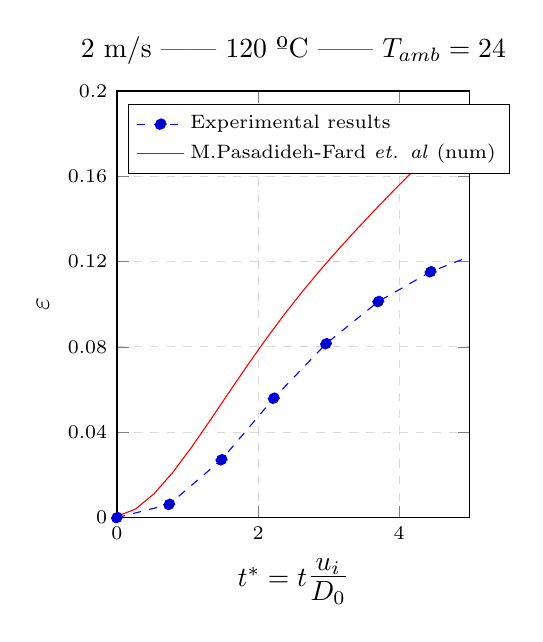
\begin{tikzpicture}
\begin{axis}[
	title = {2 m/s || 120 ºC || $T_{amb}=24$},
    tick label style={font=\scriptsize},
    legend style={font=\scriptsize,/tikz/column 2/.style={column sep=5pt},},
    %legend columns=2,
    legend cell align=left,
	legend pos =north west,
    grid=major, % Display a grid
    grid style={dashed,gray!30}, % Set the style
    xlabel={$t^*=t$\Large{$\frac{u_i}{D_0}$}},
    ylabel={$\varepsilon$}, 
    ymin = 0, ymax = 0.2,
    ytick={0,0.04,0.08,0.12,0.16,0.2},
    yticklabels={0,0.04,0.08,0.12,0.16,0.2},
    xmin = 0, xmax = 5,
    %ytick={0,1600,...,11200},
    %yticklabel style={
    %    /pgf/number format/fixed,
    %    /pgf/number format/precision=5},
	%scaled y ticks=false,
    width=0.5\textwidth, 
    height=7cm,
    cycle list name= color
    ]
\addplot+[dashed]
coordinates {(	0	,	0	)
(	0.740740741	,	0.006183436	)
(	1.481481481	,	0.027132397	)
(	2.222222222	,	0.055947222	)
(	2.962962963	,	0.081489615	)
(	3.703703704	,	0.101288971	)
(	4.444444444	,	0.115230298	)
(	5.185185185	,	0.124822088	)
(	5.925925926	,	0.131242371	)
(	6.666666667	,	0.135432275	)
(	7.407407407	,	0.138496222	)
(	8.148148148	,	0.140580511	)
(	8.888888889	,	0.14177022	)
(	9.62962963	,	0.14257969	)
(	10.37037037	,	0.143075045	)
(	11.11111111	,	0.143348662	)
(	11.85185185	,	0.143623278	)
(	12.59259259	,	0.143854086	)
(	13.33333333	,	0.143895141	)
(	14.07407407	,	0.143929706	)
(	14.81481481	,	0.144092568	)
(	15.55555556	,	0.144183357	)
(	16.2962963	,	0.144236892	)
(	17.03703704	,	0.144266432	)
(	17.77777778	,	0.144186044	)
(	18.51851852	,	0.144202142	)
(	19.25925926	,	0.144378417	)
(	20	,	0.144427272	)
(	20.74074074	,	0.144534209	)
(	21.48148148	,	0.14483881	)
(	22.22222222	,	0.145008105	)
(	22.96296296	,	0.145183721	)
(	23.7037037	,	0.145324486	)
(	24.44444444	,	0.145476178	)
(	25.18518519	,	0.145726953	)
(	25.92592593	,	0.145933468	)
(	26.66666667	,	0.146100459	)
(	27.40740741	,	0.146233525	)
(	28.14814815	,	0.146439453	)
(	28.88888889	,	0.14653441	)
(	29.62962963	,	0.146576075	)
(	30.37037037	,	0.146660443	)
(	31.11111111	,	0.146754592	)
(	31.85185185	,	0.146974795	)
(	32.59259259	,	0.147098626	)
(	33.33333333	,	0.147180226	)
(	34.07407407	,	0.147398825	)
(	34.81481481	,	0.14764873	)
(	35.55555556	,	0.147820618	)
(	36.2962963	,	0.147923815	)
(	37.03703704	,	0.148112059	)
(	37.77777778	,	0.148315615	)
(	38.51851852	,	0.148439	)
(	39.25925926	,	0.148571693	)
(	40	,	0.148709699	)
(	40.74074074	,	0.148776587	)
(	41.48148148	,	0.148849014	)
(	42.22222222	,	0.148966825	)
(	42.96296296	,	0.149264835	)
(	43.7037037	,	0	)
};
\addlegendentry{Experimental results}
\addplot[
    domain=0:5, 
    samples=20,
    color=red,
]{-1.6221*10^(-5)*x^6 + 5.5731*10^(-5)*x^5 + 1.4888*10^(-3)*x^4 - 1.2942*10^(-2)*x^3 + 3.7275*10^(-2)*x^2 + 3.8779*10^(-3)*x + 6.0277*10^(-4)};
\addlegendentry{M.Pasadideh-Fard \textit{et. al} (num)}
\end{axis}
\end{tikzpicture}}
\subfigure[Full view]{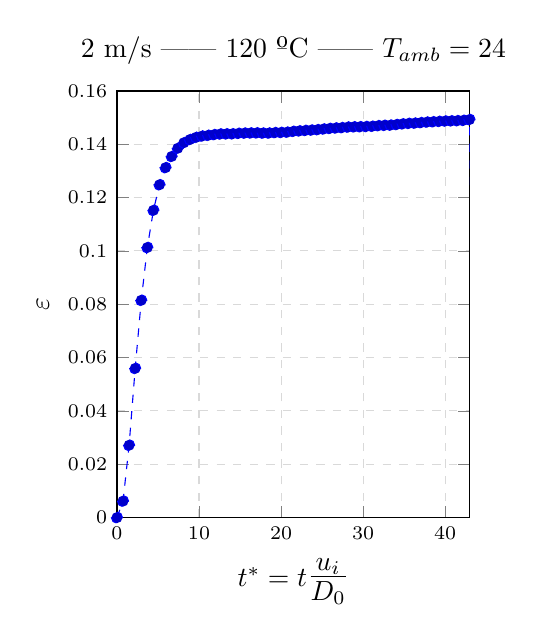
\begin{tikzpicture}
\begin{axis}[
	title = {2 m/s || 120 ºC || $T_{amb}=24$},
    tick label style={font=\scriptsize},
    legend style={font=\scriptsize,/tikz/column 2/.style={column sep=5pt},},
    %legend columns=2,
    legend cell align=left,
	legend pos =north east,
    grid=major, % Display a grid
    grid style={dashed,gray!30}, % Set the style
    xlabel={$t^*=t$\Large{$\frac{u_i}{D_0}$}},
    ylabel={$\varepsilon$}, 
    ymin = 0, ymax = 0.16,
    ytick={0,0.02,0.04,0.06,0.08,0.1,0.12,0.14,0.16},
    yticklabels={0,0.02,0.04,0.06,0.08,0.1,0.12,0.14,0.16},
    xmin = 0, xmax = 43,
    %ytick={0,1600,...,11200},
    %yticklabel style={
    %    /pgf/number format/fixed,
    %    /pgf/number format/precision=5},
	%scaled y ticks=false,
    width=0.5\textwidth, 
    height=7cm,
    cycle list name= color
    ]
\addplot+[dashed]
coordinates {(	0	,	0	)
(	0.740740741	,	0.006183436	)
(	1.481481481	,	0.027132397	)
(	2.222222222	,	0.055947222	)
(	2.962962963	,	0.081489615	)
(	3.703703704	,	0.101288971	)
(	4.444444444	,	0.115230298	)
(	5.185185185	,	0.124822088	)
(	5.925925926	,	0.131242371	)
(	6.666666667	,	0.135432275	)
(	7.407407407	,	0.138496222	)
(	8.148148148	,	0.140580511	)
(	8.888888889	,	0.14177022	)
(	9.62962963	,	0.14257969	)
(	10.37037037	,	0.143075045	)
(	11.11111111	,	0.143348662	)
(	11.85185185	,	0.143623278	)
(	12.59259259	,	0.143854086	)
(	13.33333333	,	0.143895141	)
(	14.07407407	,	0.143929706	)
(	14.81481481	,	0.144092568	)
(	15.55555556	,	0.144183357	)
(	16.2962963	,	0.144236892	)
(	17.03703704	,	0.144266432	)
(	17.77777778	,	0.144186044	)
(	18.51851852	,	0.144202142	)
(	19.25925926	,	0.144378417	)
(	20	,	0.144427272	)
(	20.74074074	,	0.144534209	)
(	21.48148148	,	0.14483881	)
(	22.22222222	,	0.145008105	)
(	22.96296296	,	0.145183721	)
(	23.7037037	,	0.145324486	)
(	24.44444444	,	0.145476178	)
(	25.18518519	,	0.145726953	)
(	25.92592593	,	0.145933468	)
(	26.66666667	,	0.146100459	)
(	27.40740741	,	0.146233525	)
(	28.14814815	,	0.146439453	)
(	28.88888889	,	0.14653441	)
(	29.62962963	,	0.146576075	)
(	30.37037037	,	0.146660443	)
(	31.11111111	,	0.146754592	)
(	31.85185185	,	0.146974795	)
(	32.59259259	,	0.147098626	)
(	33.33333333	,	0.147180226	)
(	34.07407407	,	0.147398825	)
(	34.81481481	,	0.14764873	)
(	35.55555556	,	0.147820618	)
(	36.2962963	,	0.147923815	)
(	37.03703704	,	0.148112059	)
(	37.77777778	,	0.148315615	)
(	38.51851852	,	0.148439	)
(	39.25925926	,	0.148571693	)
(	40	,	0.148709699	)
(	40.74074074	,	0.148776587	)
(	41.48148148	,	0.148849014	)
(	42.22222222	,	0.148966825	)
(	42.96296296	,	0.149264835	)
(	43.7037037	,	0	)
};
%\addlegendentry{2 m/s}
\end{axis}
\end{tikzpicture}}
\caption{Cooling effectiveness along $t^*$ for a water droplet impacting on an hydrophilic surface}
\label{fig:coolex}
\end{figure}

\subsection{Influence of the impact velocity}

\par For an hydrophilic surface (the stainless steel foil), results were taken for different impact velocities: 0.8 m/s, 2 m/s at an initial heating of 100ºC. At this temperature, boiling of the lamella is not yet observed. The two impact velocities are compared in Figure \ref{fig:hsspeed} The obvious difference is observed between the droplet spreading at different impact velocities is the spreading diameter, which is directly influenced by the impact velocity. One of the differences is the fingering, that only happens for 2 m/s (at t= 6ms). The height of the lamella is also smaller for this velocity.\\

\begin{figure}[h]
\centering
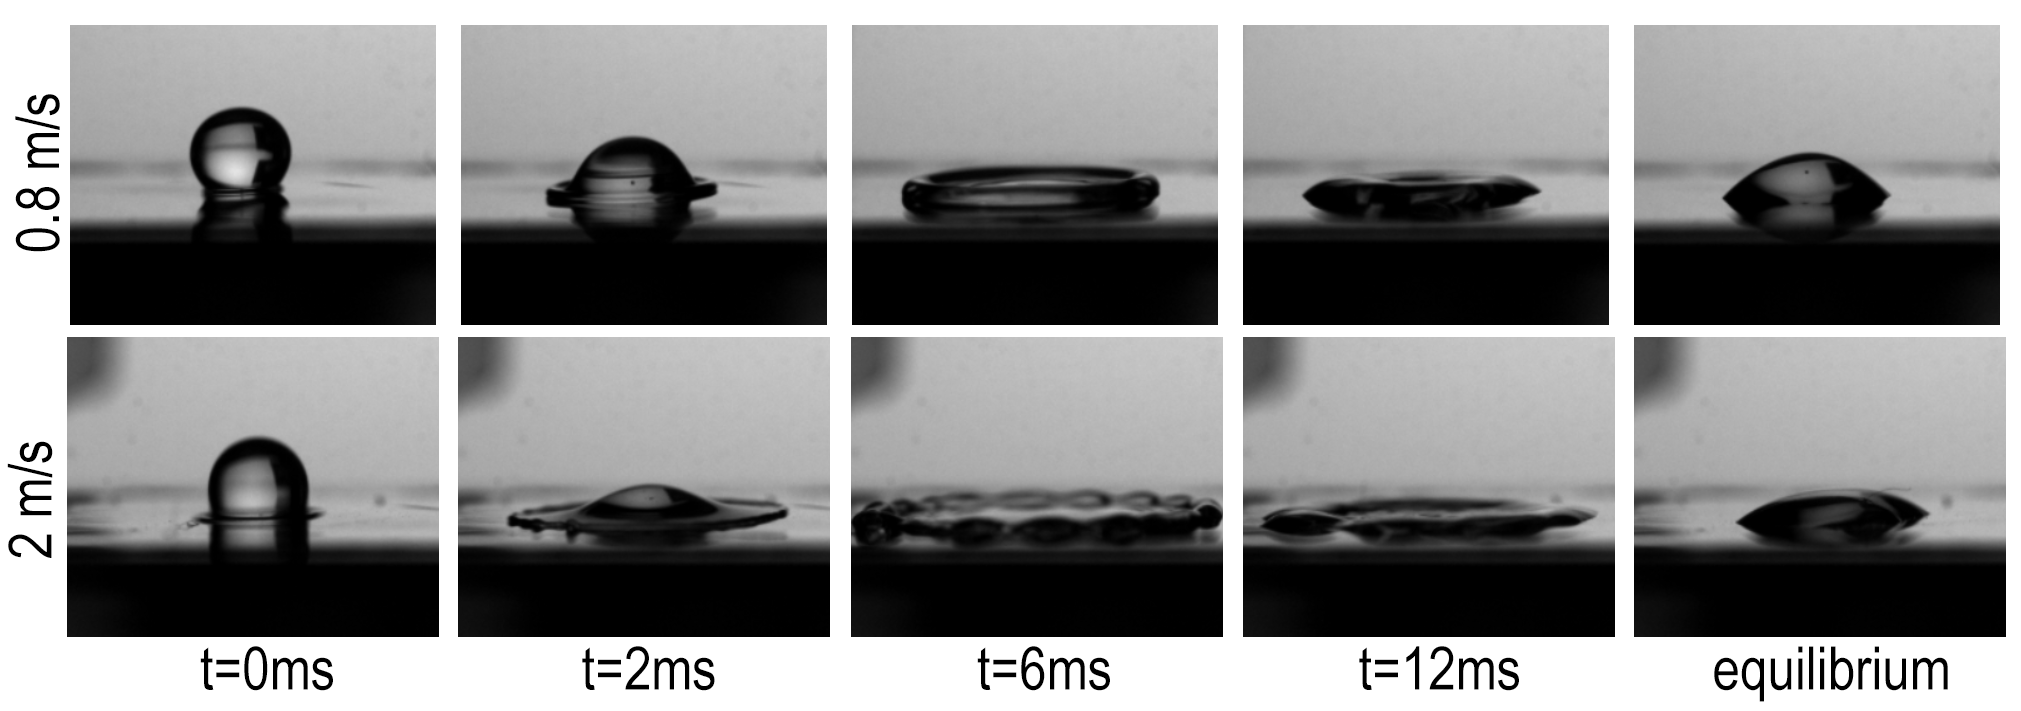
\includegraphics[width=1\linewidth]{Figures/5.Chapter/hsspeed.png}
\caption{Comparison of droplet impact at 0.8m/s and 2m/s. The water droplet impacts the surface at an initial temperature of 100ºC}
\label{fig:hsspeed}
\end{figure}

\par Using the high speed camera it was possible to extract the droplet diameter for each frame, with the help of a code developed previously by Tomás Valente. The comparison between the spreading factor of each velocity can be seen in Figure \ref{fig:diameter}. As expected the spreading factor grows more with a higher impact velocity. In this figure the difference between the maximum diameter time can be compared. In the case of 2 m/s the time in which the maximum diameter occurs is at approximately 4 ms, and in the case of 0.8 m/s occurs at 6 ms. The spreading factor difference in maximum diameter has a relation of approximately 2,5 to 4, which is considerably larger.\\

\begin{figure}[h]
\centering
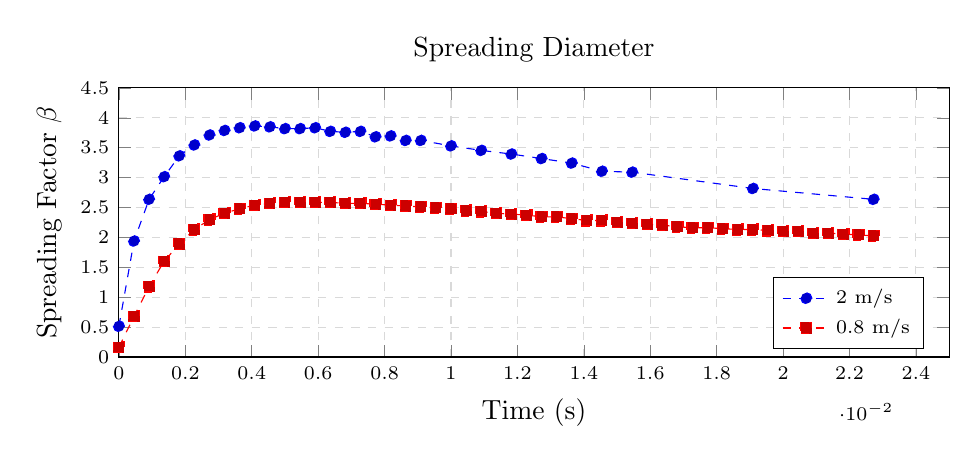
\begin{tikzpicture}
\begin{axis}[
	title = {Spreading Diameter},
    tick label style={font=\scriptsize},
    legend style={font=\scriptsize,/tikz/column 2/.style={column sep=5pt},},
    %legend columns=2,
    legend cell align=left,
	legend pos =south east,
    grid=major, % Display a grid
    grid style={dashed,gray!30}, % Set the style
    xlabel={Time (s)},
    ylabel={Spreading Factor $\beta$}, 
    ymin = 0, ymax = 4.5,
    ytick={0,0.5,...,4.5},
    %yticklabels={300,325,350,375,400,425,450,475,500,525},
    xmin = 0, xmax = 0.025,
    %ytick={0,1600,...,11200},
    %yticklabel style={
    %    /pgf/number format/fixed,
    %    /pgf/number format/precision=5},
	%scaled y ticks=false,
    width=1\textwidth, height=5cm,
    cycle list name= color
    ]
\addplot+[dashed]
coordinates {(	0	,	0.515151515	)
(	0.000454545	,	1.939393939	)
(	0.000909091	,	2.636363636	)
(	0.001363636	,	3.015151515	)
(	0.001818182	,	3.363636364	)
(	0.002272727	,	3.545454545	)
(	0.002727273	,	3.712121212	)
(	0.003181818	,	3.787878788	)
(	0.003636364	,	3.833333333	)
(	0.004090909	,	3.863636364	)
(	0.004545455	,	3.848484848	)
(	0.005	,	3.818181818	)
(	0.005454545	,	3.818181818	)
(	0.005909091	,	3.833333333	)
(	0.006363636	,	3.772727273	)
(	0.006818182	,	3.757575758	)
(	0.007272727	,	3.772727273	)
(	0.007727273	,	3.681818182	)
(	0.008181818	,	3.696969697	)
(	0.008636364	,	3.621212121	)
(	0.009090909	,	3.621212121	)
(	0.01	,	3.53030303	)
(	0.010909091	,	3.454545455	)
(	0.011818182	,	3.393939394	)
(	0.012727273	,	3.318181818	)
(	0.013636364	,	3.242424242	)
(	0.014545455	,	3.106060606	)
(	0.015454545	,	3.090909091	)
(	0.019090909	,	2.818181818	)
(	0.022727273	,	2.636363636	)
};
\addlegendentry{2 m/s}

\addplot+[dashed]
coordinates {(	0	,	0.166303558	)
(	0.000454545	,	0.680332739	)
(	0.000909091	,	1.179243415	)
(	0.001363636	,	1.602561563	)
(	0.001818182	,	1.889813164	)
(	0.002272727	,	2.131709249	)
(	0.002727273	,	2.298012808	)
(	0.003181818	,	2.403842345	)
(	0.003636364	,	2.479434872	)
(	0.004090909	,	2.539908893	)
(	0.004545455	,	2.570145903	)
(	0.005	,	2.585264409	)
(	0.005454545	,	2.585264409	)
(	0.005909091	,	2.585264409	)
(	0.006363636	,	2.585264409	)
(	0.006818182	,	2.570145903	)
(	0.007272727	,	2.570145903	)
(	0.007727273	,	2.555027398	)
(	0.008181818	,	2.539908893	)
(	0.008636364	,	2.524790388	)
(	0.009090909	,	2.509671882	)
(	0.009545455	,	2.494553377	)
(	0.01	,	2.479434872	)
(	0.010454545	,	2.449197861	)
(	0.010909091	,	2.434079356	)
(	0.011363636	,	2.403842345	)
(	0.011818182	,	2.38872384	)
(	0.012272727	,	2.373605334	)
(	0.012727273	,	2.343368324	)
(	0.013181818	,	2.343368324	)
(	0.013636364	,	2.313131313	)
(	0.014090909	,	2.282894303	)
(	0.014545455	,	2.282894303	)
(	0.015	,	2.252657292	)
(	0.015454545	,	2.237538787	)
(	0.015909091	,	2.222420281	)
(	0.016363636	,	2.207301776	)
(	0.016818182	,	2.177064765	)
(	0.017272727	,	2.16194626	)
(	0.017727273	,	2.16194626	)
(	0.018181818	,	2.146827755	)
(	0.018636364	,	2.131709249	)
(	0.019090909	,	2.131709249	)
(	0.019545455	,	2.116590744	)
(	0.02	,	2.101472239	)
(	0.020454545	,	2.101472239	)
(	0.020909091	,	2.071235228	)
(	0.021363636	,	2.071235228	)
(	0.021818182	,	2.056116723	)
(	0.022272727	,	2.040998217	)
(	0.022727273	,	2.025879712	)
};
\addlegendentry{0.8 m/s}

\end{axis}
\end{tikzpicture}
\caption{Comparison between the spreading factor of each velocity}
\label{fig:diameter}
\end{figure}
\begin{figure}[h!]
\centering
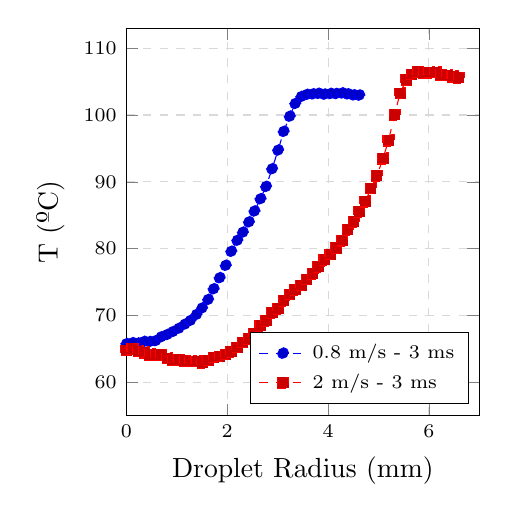
\begin{tikzpicture}
\begin{axis}[
	%title = {107 ºC || $T_{amb}=24$},
    tick label style={font=\scriptsize},
    legend style={font=\scriptsize,/tikz/column 2/.style={column sep=5pt},},
    %legend columns=2,
    legend cell align=left,
	legend pos =south east,
    grid=major, % Display a grid
    grid style={dashed,gray!30}, % Set the style
    xlabel={Droplet Radius (mm)},
    ylabel={T (ºC)}, 
    ymin = 55, ymax = 113,
    ytick={60,70,...,100,110},
    %yticklabels={300,325,350,375,400,425,450,475,500,525},
    xmin = 0, xmax = 7,
    %ytick={0,1600,...,11200},
    %yticklabel style={
    %    /pgf/number format/fixed,
    %    /pgf/number format/precision=5},
	%scaled y ticks=false,
    width=0.5\textwidth, height=6.5cm,
    cycle list name= color
    ]
\addplot+[dashed]
coordinates {(	0	,	65.76	)
(	0.12	,	65.9	)
(	0.23	,	65.85	)
(	0.35	,	66.09	)
(	0.46	,	66.07	)
(	0.58	,	66.22	)
(	0.69	,	66.79	)
(	0.81	,	67.14	)
(	0.92	,	67.57	)
(	1.04	,	68.07	)
(	1.16	,	68.69	)
(	1.27	,	69.25	)
(	1.39	,	70.14	)
(	1.5	,	71.11	)
(	1.62	,	72.38	)
(	1.73	,	73.98	)
(	1.85	,	75.64	)
(	1.97	,	77.5	)
(	2.08	,	79.6	)
(	2.2	,	81.25	)
(	2.31	,	82.46	)
(	2.43	,	84	)
(	2.54	,	85.63	)
(	2.66	,	87.47	)
(	2.77	,	89.31	)
(	2.89	,	91.96	)
(	3.01	,	94.76	)
(	3.12	,	97.56	)
(	3.24	,	99.83	)
(	3.35	,	101.74	)
(	3.47	,	102.78	)
(	3.58	,	103.09	)
(	3.7	,	103.17	)
(	3.81	,	103.25	)
(	3.93	,	103.13	)
(	4.05	,	103.23	)
(	4.16	,	103.22	)
(	4.28	,	103.31	)
(	4.39	,	103.17	)
(	4.51	,	103.02	)
(	4.62	,	102.99	)
};
\addlegendentry{0.8 m/s - 3 ms}

\addplot+[dashed]
coordinates {(	0	,	64.76	)
(	0.12	,	64.97	)
(	0.23	,	64.61	)
(	0.35	,	64.44	)
(	0.46	,	64.13	)
(	0.58	,	64.08	)
(	0.69	,	64.09	)
(	0.81	,	63.56	)
(	0.92	,	63.26	)
(	1.04	,	63.34	)
(	1.16	,	63.22	)
(	1.27	,	63.12	)
(	1.39	,	63.12	)
(	1.5	,	62.93	)
(	1.62	,	63.29	)
(	1.73	,	63.7	)
(	1.85	,	63.88	)
(	1.97	,	64.17	)
(	2.08	,	64.58	)
(	2.2	,	65.21	)
(	2.31	,	65.97	)
(	2.43	,	66.51	)
(	2.54	,	67.27	)
(	2.66	,	68.47	)
(	2.77	,	69.17	)
(	2.89	,	70.41	)
(	3.01	,	71.01	)
(	3.12	,	72.19	)
(	3.24	,	73.14	)
(	3.35	,	73.85	)
(	3.47	,	74.52	)
(	3.58	,	75.4	)
(	3.7	,	76.25	)
(	3.81	,	77.3	)
(	3.93	,	78.35	)
(	4.05	,	79.18	)
(	4.16	,	80.08	)
(	4.28	,	81.21	)
(	4.39	,	82.8	)
(	4.51	,	84	)
(	4.62	,	85.5	)
(	4.74	,	87.06	)
(	4.85	,	89.03	)
(	4.97	,	90.91	)
(	5.09	,	93.49	)
(	5.2	,	96.19	)
(	5.32	,	100.05	)
(	5.43	,	103.28	)
(	5.55	,	105.25	)
(	5.66	,	106.11	)
(	5.78	,	106.44	)
(	5.9	,	106.29	)
(	6.01	,	106.37	)
(	6.13	,	106.42	)
(	6.24	,	106	)
(	6.36	,	105.96	)
(	6.47	,	105.78	)
(	6.59	,	105.59	)
};
\addlegendentry{2 m/s - 3 ms}

\end{axis}
\end{tikzpicture}
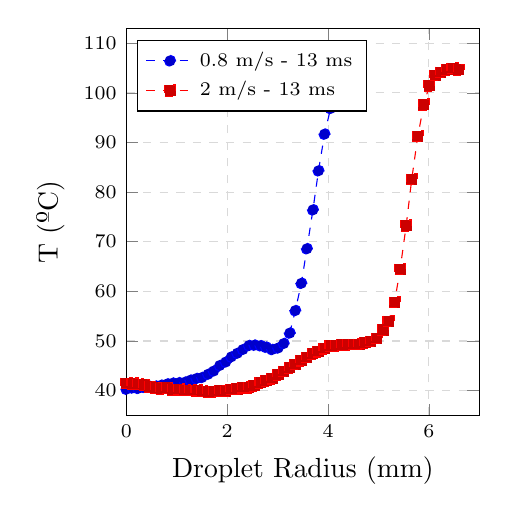
\begin{tikzpicture}
\begin{axis}[
	%title = {107 ºC || $T_{amb}=24$},
    tick label style={font=\scriptsize},
    legend style={font=\scriptsize,/tikz/column 2/.style={column sep=5pt},},
    %legend columns=2,
    legend cell align=left,
	legend pos =north west,
    grid=major, % Display a grid
    grid style={dashed,gray!30}, % Set the style
    xlabel={Droplet Radius (mm)},
    ylabel={T (ºC)}, 
    ymin = 35, ymax = 113,
    ytick={30,40,...,100,110},
    %yticklabels={300,325,350,375,400,425,450,475,500,525},
    xmin = 0, xmax = 7,
    %ytick={0,1600,...,11200},
    %yticklabel style={
    %    /pgf/number format/fixed,
    %    /pgf/number format/precision=5},
	%scaled y ticks=false,
    width=0.5\textwidth, height=6.5cm,
    cycle list name= color
    ]
\addplot+[dashed]
coordinates {(	0	,	40.31	)
(	0.12	,	40.55	)
(	0.23	,	40.46	)
(	0.35	,	40.67	)
(	0.46	,	40.82	)
(	0.58	,	40.91	)
(	0.69	,	41.1	)
(	0.81	,	41.36	)
(	0.92	,	41.52	)
(	1.04	,	41.6	)
(	1.16	,	41.71	)
(	1.27	,	42.12	)
(	1.39	,	42.45	)
(	1.5	,	42.66	)
(	1.62	,	43.31	)
(	1.73	,	43.95	)
(	1.85	,	45.07	)
(	1.97	,	45.77	)
(	2.08	,	46.81	)
(	2.2	,	47.54	)
(	2.31	,	48.29	)
(	2.43	,	49.09	)
(	2.54	,	49.17	)
(	2.66	,	49.05	)
(	2.77	,	48.75	)
(	2.89	,	48.29	)
(	3.01	,	48.6	)
(	3.12	,	49.5	)
(	3.24	,	51.61	)
(	3.35	,	56.13	)
(	3.47	,	61.63	)
(	3.58	,	68.59	)
(	3.7	,	76.42	)
(	3.81	,	84.29	)
(	3.93	,	91.67	)
(	4.05	,	96.84	)
(	4.16	,	100.05	)
(	4.28	,	101.53	)
(	4.39	,	102.28	)
(	4.51	,	102.08	)
(	4.62	,	101.62	)
};
\addlegendentry{0.8 m/s - 13 ms}

\addplot+[dashed]
coordinates {(	0	,	41.51	)
(	0.12	,	41.44	)
(	0.23	,	41.31	)
(	0.35	,	41.14	)
(	0.46	,	40.77	)
(	0.58	,	40.61	)
(	0.69	,	40.39	)
(	0.81	,	40.57	)
(	0.92	,	40.22	)
(	1.04	,	40.24	)
(	1.16	,	40.11	)
(	1.27	,	40.11	)
(	1.39	,	40.05	)
(	1.5	,	39.87	)
(	1.62	,	39.81	)
(	1.73	,	39.79	)
(	1.85	,	39.95	)
(	1.97	,	39.91	)
(	2.08	,	40.28	)
(	2.2	,	40.34	)
(	2.31	,	40.64	)
(	2.43	,	40.65	)
(	2.54	,	41.02	)
(	2.66	,	41.57	)
(	2.77	,	41.97	)
(	2.89	,	42.46	)
(	3.01	,	43.23	)
(	3.12	,	43.95	)
(	3.24	,	44.59	)
(	3.35	,	45.3	)
(	3.47	,	46.08	)
(	3.58	,	46.71	)
(	3.7	,	47.43	)
(	3.81	,	47.91	)
(	3.93	,	48.5	)
(	4.05	,	49.05	)
(	4.16	,	49.05	)
(	4.28	,	49.21	)
(	4.39	,	49.27	)
(	4.51	,	49.33	)
(	4.62	,	49.37	)
(	4.74	,	49.62	)
(	4.85	,	49.94	)
(	4.97	,	50.54	)
(	5.09	,	52.22	)
(	5.2	,	54.01	)
(	5.32	,	57.83	)
(	5.43	,	64.46	)
(	5.55	,	73.26	)
(	5.66	,	82.58	)
(	5.78	,	91.23	)
(	5.9	,	97.63	)
(	6.01	,	101.44	)
(	6.13	,	103.55	)
(	6.24	,	104.15	)
(	6.36	,	104.67	)
(	6.47	,	104.97	)
(	6.59	,	104.65	)
};
\addlegendentry{2 m/s - 13 ms}
\end{axis}
\end{tikzpicture}
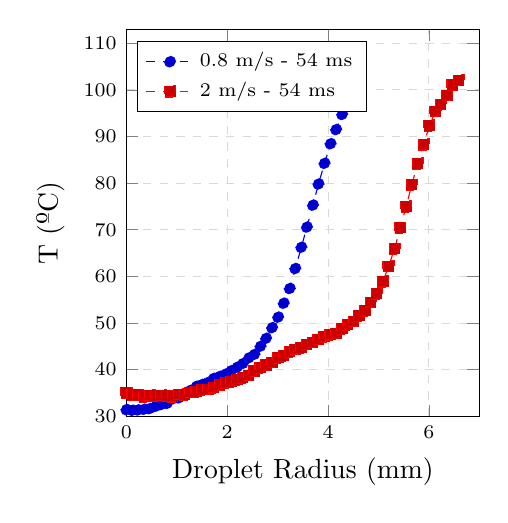
\begin{tikzpicture}
\begin{axis}[
	%
    tick label style={font=\scriptsize},
    legend style={font=\scriptsize,/tikz/column 2/.style={column sep=5pt},},
    %legend columns=2,
    legend cell align=left,
	legend pos =north west,
    grid=major, % Display a grid
    grid style={dashed,gray!30}, % Set the style
    xlabel={Droplet Radius (mm)},
    ylabel={T (ºC)}, 
    ymin = 30, ymax = 113,
    ytick={30,40,...,100,110},
    %yticklabels={300,325,350,375,400,425,450,475,500,525},
    xmin = 0, xmax = 7,
    %ytick={0,1600,...,11200},
    %yticklabel style={
    %    /pgf/number format/fixed,
    %    /pgf/number format/precision=5},
	%scaled y ticks=false,
    width=0.5\textwidth, height=6.5cm,
    cycle list name= color
    ]
\addplot+[dashed]
coordinates {(	0	,	31.46	)
(	0.12	,	31.32	)
(	0.23	,	31.38	)
(	0.35	,	31.53	)
(	0.46	,	31.66	)
(	0.58	,	32.15	)
(	0.69	,	32.52	)
(	0.81	,	32.8	)
(	0.92	,	33.75	)
(	1.04	,	33.96	)
(	1.16	,	35	)
(	1.27	,	35.59	)
(	1.39	,	36.46	)
(	1.5	,	36.84	)
(	1.62	,	37.3	)
(	1.73	,	38.14	)
(	1.85	,	38.58	)
(	1.97	,	39.1	)
(	2.08	,	39.81	)
(	2.2	,	40.56	)
(	2.31	,	41.33	)
(	2.43	,	42.55	)
(	2.54	,	43.29	)
(	2.66	,	45.03	)
(	2.77	,	46.72	)
(	2.89	,	49.02	)
(	3.01	,	51.27	)
(	3.12	,	54.26	)
(	3.24	,	57.42	)
(	3.35	,	61.69	)
(	3.47	,	66.25	)
(	3.58	,	70.58	)
(	3.7	,	75.28	)
(	3.81	,	79.81	)
(	3.93	,	84.25	)
(	4.05	,	88.44	)
(	4.16	,	91.48	)
(	4.28	,	94.72	)
(	4.39	,	97	)
(	4.51	,	98.21	)
(	4.62	,	99.1	)
};
\addlegendentry{0.8 m/s - 54 ms}

\addplot+[dashed]
coordinates {(	0	,	35.05	)
(	0.12	,	34.63	)
(	0.23	,	34.58	)
(	0.35	,	34.24	)
(	0.46	,	34.48	)
(	0.58	,	34.4	)
(	0.69	,	34.56	)
(	0.81	,	34.42	)
(	0.92	,	34.26	)
(	1.04	,	34.72	)
(	1.16	,	34.6	)
(	1.27	,	35.17	)
(	1.39	,	35.31	)
(	1.5	,	35.71	)
(	1.62	,	35.84	)
(	1.73	,	36.19	)
(	1.85	,	36.73	)
(	1.97	,	37.22	)
(	2.08	,	37.44	)
(	2.2	,	37.85	)
(	2.31	,	38.32	)
(	2.43	,	38.85	)
(	2.54	,	39.73	)
(	2.66	,	40.45	)
(	2.77	,	41.01	)
(	2.89	,	41.65	)
(	3.01	,	42.6	)
(	3.12	,	43.01	)
(	3.24	,	43.82	)
(	3.35	,	44.37	)
(	3.47	,	44.7	)
(	3.58	,	45.48	)
(	3.7	,	45.91	)
(	3.81	,	46.53	)
(	3.93	,	47.14	)
(	4.05	,	47.55	)
(	4.16	,	47.86	)
(	4.28	,	48.81	)
(	4.39	,	49.67	)
(	4.51	,	50.37	)
(	4.62	,	51.56	)
(	4.74	,	52.65	)
(	4.85	,	54.44	)
(	4.97	,	56.31	)
(	5.09	,	58.93	)
(	5.2	,	62.17	)
(	5.32	,	65.89	)
(	5.43	,	70.41	)
(	5.55	,	74.98	)
(	5.66	,	79.66	)
(	5.78	,	84.19	)
(	5.9	,	88.29	)
(	6.01	,	92.34	)
(	6.13	,	95.38	)
(	6.24	,	96.93	)
(	6.36	,	98.86	)
(	6.47	,	101.02	)
(	6.59	,	102.02	)
};
\addlegendentry{2 m/s - 54 ms}

\end{axis}
\end{tikzpicture}
\caption{Average temperature along the radius between the 5 experiments of both velocity values at 100ºC}
\label{fig:speed1}
\end{figure}

\par Lets now take a look at the influence of the velocity in the temperature field. In Figure \ref{fig:speed1}, the average of all experiments made for both velocity values at 100ºC is presented for comparison. The temperature at the center of the droplet is similar during the spreading (3ms and 13 ms). The temperature at the droplet center drops more intensely in the lower velocity. This is justified by the height difference, also noticeable in the last panel of Figure \ref{fig:irvshr}. Looking at the shape of the curves, one can observe their similarity.\\

\par The temperature fields can only give us qualitative information. To quantify cooling and compare both velocities, the heat flux and cooling effectiveness should be considered. Starting with the heat flux, the measurements made for an droplet impacting on a hydrophilic surface at initial temperature of 120ºC were taken as an example. The comparison between different impact velocities is shown in Figure \ref{fig:speedflux}. For both time frames, the contact edge can be easily identified, and the same phenomena are present: the contact edge peak, the peak and drop of the flux caused by the lamella's rim and the heat flux drop in the center due to the trapped gas bubble effect. Overall the flux is higher in the 2 m/s due to the wetted area being larger. The fact that the lamella is thinner in the 2 m/s impact velocity tests, is compensated by the increase in convection heat transfer. As seen before, when reaching equilibrium, the lamella is hotter for the 2 m/s measurements. This is the cause of having a thinner lamella with greater heat flux promoted by convection, which heats the droplet to higher temperatures than in the 0.8 m/s impact velocity case study. This can be also related to the fact that even though the lamella thickness is higher in lower velocities, the heat flux is comparable or even lower, as seen in the figure.\\

\begin{figure}[h!]
\centering
\subfigure[t=2ms]{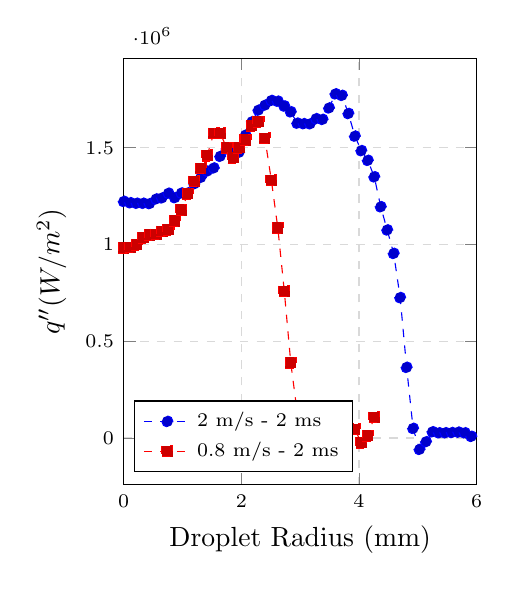
\begin{tikzpicture}
\begin{axis}[
	%title = {107 ºC || $T_{amb}=24$},
    tick label style={font=\scriptsize},
    legend style={font=\scriptsize,/tikz/column 2/.style={column sep=5pt},},
    %legend columns=2,
    legend cell align=left,
	legend pos =south west,
    grid=major, % Display a grid
    grid style={dashed,gray!30}, % Set the style
    xlabel={Droplet Radius (mm)},
    ylabel={$q''(W/m^2)$}, 
    %ymin = 55, ymax = 113,
    %ytick={60,70,...,100,110},
    %yticklabels={300,325,350,375,400,425,450,475,500,525},
    xmin = 0, xmax = 6,
    %ytick={0,1600,...,11200},
    %yticklabel style={
    %    /pgf/number format/fixed,
    %    /pgf/number format/precision=5},
	%scaled y ticks=false,
    width=0.5\textwidth, height=7cm,
    cycle list name= color
    ]
\addplot+[dashed]
coordinates {(	0	,	1222928.282	)
(	0.11	,	1215849.141	)
(	0.22	,	1213084.596	)
(	0.33	,	1213086.158	)
(	0.44	,	1211400.892	)
(	0.55	,	1235404.245	)
(	0.65	,	1240861.278	)
(	0.76	,	1265052.878	)
(	0.87	,	1242151.87	)
(	0.98	,	1266289.273	)
(	1.09	,	1267085.873	)
(	1.2	,	1313566.011	)
(	1.31	,	1346458.22	)
(	1.42	,	1379273.853	)
(	1.53	,	1395499.139	)
(	1.64	,	1456019.173	)
(	1.75	,	1493810.865	)
(	1.86	,	1473581.581	)
(	1.96	,	1476135.892	)
(	2.07	,	1565916.03	)
(	2.18	,	1634801.538	)
(	2.29	,	1694731.24	)
(	2.4	,	1720340.631	)
(	2.51	,	1744493.418	)
(	2.62	,	1740517.709	)
(	2.73	,	1715786.56	)
(	2.84	,	1685690.399	)
(	2.95	,	1627167.242	)
(	3.06	,	1624506.602	)
(	3.17	,	1624035.892	)
(	3.27	,	1650388.938	)
(	3.38	,	1646634.982	)
(	3.49	,	1705826.365	)
(	3.6	,	1778766.58	)
(	3.71	,	1770709.96	)
(	3.82	,	1677101.721	)
(	3.93	,	1560263.745	)
(	4.04	,	1485161.428	)
(	4.15	,	1434901.368	)
(	4.26	,	1349939.93	)
(	4.37	,	1195111.19	)
(	4.48	,	1075263.809	)
(	4.59	,	953854.8961	)
(	4.7	,	725686.3235	)
(	4.81	,	364954.9878	)
(	4.92	,	49503.72871	)
(	5.03	,	-59084.16501	)
(	5.14	,	-19531.08151	)
(	5.25	,	32022.35363	)
(	5.36	,	26527.29569	)
(	5.47	,	26988.35026	)
(	5.58	,	27913.49288	)
(	5.69	,	30025.61937	)
(	5.8	,	26521.48957	)
(	5.91	,	8018.877223	)
(	6.02	,	23268.75141	)
(	6.13	,	37250.24771	)
(	6.24	,	45560.10852	)
(	6.35	,	45238.34546	)
(	6.46	,	33697.84031	)
};
\addlegendentry{2 m/s - 2 ms}

\addplot+[dashed]
coordinates {(	0	,	982089.2242	)
(	0.11	,	986559.7305	)
(	0.22	,	999747.4309	)
(	0.33	,	1035364.347	)
(	0.44	,	1049283.945	)
(	0.55	,	1053120.393	)
(	0.65	,	1068631.742	)
(	0.76	,	1076954.643	)
(	0.87	,	1121386.9	)
(	0.98	,	1178256.05	)
(	1.09	,	1261378.47	)
(	1.2	,	1327056.42	)
(	1.31	,	1393696.902	)
(	1.42	,	1460274.884	)
(	1.53	,	1574936.222	)
(	1.64	,	1575660.786	)
(	1.75	,	1499525.579	)
(	1.86	,	1449022.358	)
(	1.96	,	1499662.339	)
(	2.07	,	1540313.795	)
(	2.18	,	1614313.74	)
(	2.29	,	1635300.374	)
(	2.4	,	1549877.215	)
(	2.51	,	1331868.982	)
(	2.62	,	1085363.344	)
(	2.73	,	759206.8787	)
(	2.84	,	388588.3723	)
(	2.95	,	131341.4508	)
(	3.06	,	-34143.38797	)
(	3.17	,	-49030.87567	)
(	3.27	,	-37679.13294	)
(	3.38	,	73913.01076	)
(	3.49	,	47158.40863	)
(	3.6	,	18684.75783	)
(	3.71	,	-12798.88057	)
(	3.82	,	44948.25807	)
(	3.93	,	45229.68041	)
(	4.04	,	-25391.89314	)
(	4.15	,	12194.80767	)
(	4.26	,	107861.5786	)
};
\addlegendentry{0.8 m/s - 2 ms}
\end{axis}
\end{tikzpicture}}
\subfigure[t=4ms]{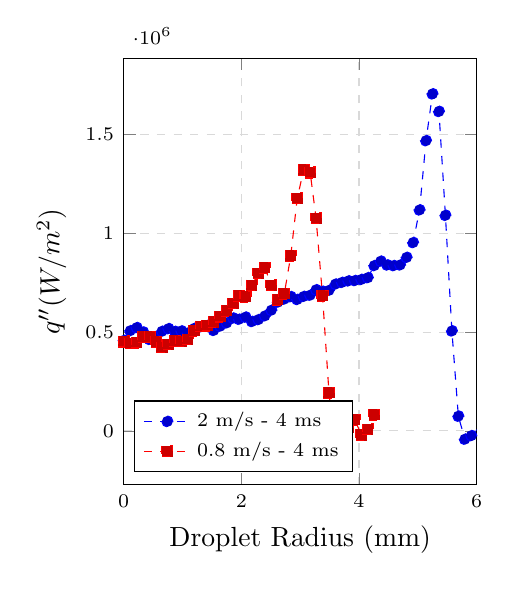
\begin{tikzpicture}
\begin{axis}[
	%title = {107 ºC || $T_{amb}=24$},
    tick label style={font=\scriptsize},
    legend style={font=\scriptsize,/tikz/column 2/.style={column sep=5pt},},
    %legend columns=2,
    legend cell align=left,
	legend pos =south west,
    grid=major, % Display a grid
    grid style={dashed,gray!30}, % Set the style
    xlabel={Droplet Radius (mm)},
    ylabel={$q''(W/m^2)$}, 
    %ymin = 55, ymax = 113,
    %ytick={60,70,...,100,110},
    %yticklabels={300,325,350,375,400,425,450,475,500,525},
    xmin = 0, xmax = 6,
    %ytick={0,1600,...,11200},
    %yticklabel style={
    %    /pgf/number format/fixed,
    %    /pgf/number format/precision=5},
	%scaled y ticks=false,
    width=0.5\textwidth, height=7cm,
    cycle list name= color
    ]
\addplot+[dashed]
coordinates {(	0	,	457891.6753	)
(	0.11	,	507064.9899	)
(	0.22	,	522910.9379	)
(	0.33	,	500242.4852	)
(	0.44	,	463365.0432	)
(	0.55	,	478442.7874	)
(	0.65	,	504285.7831	)
(	0.76	,	517686.3029	)
(	0.87	,	503481.8026	)
(	0.98	,	506001.1791	)
(	1.09	,	496101.8141	)
(	1.2	,	519287.9102	)
(	1.31	,	527127.0695	)
(	1.42	,	533543.4318	)
(	1.53	,	508658.7927	)
(	1.64	,	530029.7099	)
(	1.75	,	546459.349	)
(	1.86	,	571068.3205	)
(	1.96	,	565131.6119	)
(	2.07	,	576074.2389	)
(	2.18	,	553638.8588	)
(	2.29	,	563481.4723	)
(	2.4	,	582316.0827	)
(	2.51	,	610945.4134	)
(	2.62	,	651513.1628	)
(	2.73	,	667209.4191	)
(	2.84	,	679361.1877	)
(	2.95	,	665263.4826	)
(	3.06	,	680632.1803	)
(	3.17	,	687074.987	)
(	3.27	,	714406.5351	)
(	3.38	,	706623.7493	)
(	3.49	,	711358.7953	)
(	3.6	,	743258.2312	)
(	3.71	,	751652.0158	)
(	3.82	,	759377.5672	)
(	3.93	,	761043.1969	)
(	4.04	,	766680.3584	)
(	4.15	,	775528.0512	)
(	4.26	,	836902.633	)
(	4.37	,	859092.122	)
(	4.48	,	839969.4348	)
(	4.59	,	836623.7019	)
(	4.7	,	840120.5396	)
(	4.81	,	878163.0386	)
(	4.92	,	953333.4713	)
(	5.03	,	1118509.827	)
(	5.14	,	1469124.162	)
(	5.25	,	1705995.515	)
(	5.36	,	1616873.685	)
(	5.47	,	1091282.204	)
(	5.58	,	506176.6586	)
(	5.69	,	74634.42136	)
(	5.8	,	-41828.93489	)
(	5.91	,	-23955.13351	)
(	6.02	,	10216.85089	)
(	6.13	,	18374.51318	)
(	6.24	,	27140.36783	)
(	6.35	,	24403.91659	)
(	6.46	,	10468.43602	)
};
\addlegendentry{2 m/s - 4 ms}

\addplot+[dashed]
coordinates {(	0	,	452958.8884	)
(	0.11	,	443672.2939	)
(	0.22	,	447691.5594	)
(	0.33	,	476523.1849	)
(	0.44	,	476471.8183	)
(	0.55	,	450806.3468	)
(	0.65	,	423782.5444	)
(	0.76	,	438179.2292	)
(	0.87	,	456897.6624	)
(	0.98	,	454134.3395	)
(	1.09	,	464286.0605	)
(	1.2	,	506555.4293	)
(	1.31	,	529832.2559	)
(	1.42	,	533809	)
(	1.53	,	551142.8174	)
(	1.64	,	579323.7681	)
(	1.75	,	608315.9539	)
(	1.86	,	645875.8736	)
(	1.96	,	683086.4821	)
(	2.07	,	680217.8765	)
(	2.18	,	737096.0515	)
(	2.29	,	797628.0866	)
(	2.4	,	826481.1812	)
(	2.51	,	736599.5618	)
(	2.62	,	663007.6906	)
(	2.73	,	693457.4194	)
(	2.84	,	886760.2203	)
(	2.95	,	1177186.265	)
(	3.06	,	1321888.579	)
(	3.17	,	1307905.114	)
(	3.27	,	1077377.636	)
(	3.38	,	683874.6368	)
(	3.49	,	192779.5452	)
(	3.6	,	-86073.52402	)
(	3.71	,	-93468.67899	)
(	3.82	,	15343.63931	)
(	3.93	,	56675.86267	)
(	4.04	,	-20794.54961	)
(	4.15	,	8059.529388	)
(	4.26	,	82566.79303	)
};
\addlegendentry{0.8 m/s - 4 ms}

\end{axis}
\end{tikzpicture}}
\caption{Comparison of the heat flux computed for different impact velocities. The water droplets impact the surface which is at an initial temperature of 120ºC}
\label{fig:speedflux}
\end{figure}

\par To study the influence of the impact velocity, the results for each velocity were plotted together, using non-dimensional time. The generated plots for the temperature at 120ºC can be seen in Figure \ref{fig:speedcool}. In a first analysis it is possible to see similar changes in the curves for different impact velocities (Figure \ref{fig:cooling}). These plots show the difference in cooling effectiveness. It is clear that the higher impact velocity impacts show more heat removal capacity that the lower velocity ones. This is not always the case though. In the first instants after impact the lower impact velocity impacts show more efficiency in removing heat. But when it comes down to the latter time steps the effectiveness more than doubles with the impact velocity.\\

\begin{figure}[h]
\subfigure[Detail]{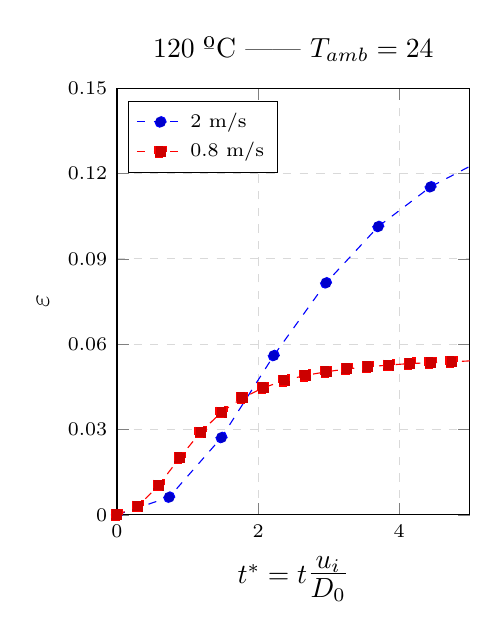
\begin{tikzpicture}
\begin{axis}[
	title = {120 ºC || $T_{amb}=24$},
    tick label style={font=\scriptsize},
    legend style={font=\scriptsize,/tikz/column 2/.style={column sep=5pt},},
    %legend columns=2,
    legend cell align=left,
	legend pos =north west,
    grid=major, % Display a grid
    grid style={dashed,gray!30}, % Set the style
    xlabel={$t^*=t$\Large{$\frac{u_i}{D_0}$}},
    ylabel={$\varepsilon$}, 
    ymin = 0, ymax = 0.15,
    ytick={0,0.03,0.06,0.09,0.12,0.15},
    yticklabels={0,0.03,0.06,0.09,0.12,0.15},
    xmin = 0, xmax = 5,
    %ytick={0,1600,...,11200},
    %yticklabel style={
    %    /pgf/number format/fixed,
    %    /pgf/number format/precision=5},
	%scaled y ticks=false,
    width=0.5\textwidth, 
    height=7cm,
    cycle list name= color
    ]
\addplot+[dashed]
coordinates {(	0	,	0	)
(	0.740740741	,	0.006204439	)
(	1.481481481	,	0.027167401	)
(	2.222222222	,	0.055996228	)
(	2.962962963	,	0.081552623	)
(	3.703703704	,	0.10136598	)
(	4.444444444	,	0.11532131	)
(	5.185185185	,	0.124927101	)
(	5.925925926	,	0.131361385	)
};
\addlegendentry{2 m/s}
\addplot+[dashed]
coordinates {(	0	,	0	)
(	0.296296296	,	0.003018616	)
(	0.592592593	,	0.010388567	)
(	0.888888889	,	0.020058751	)
(	1.185185185	,	0.029057225	)
(	1.481481481	,	0.036086665	)
(	1.777777778	,	0.041101457	)
(	2.074074074	,	0.044656137	)
(	2.37037037	,	0.047221941	)
(	2.666666667	,	0.04900349	)
(	2.962962963	,	0.050282037	)
(	3.259259259	,	0.051294611	)
(	3.555555556	,	0.052024343	)
(	3.851851852	,	0.052657377	)
(	4.148148148	,	0.053180309	)
(	4.444444444	,	0.053460793	)
(	4.740740741	,	0.053762748	)
(	5.037037037	,	0.05417938	)
};
\addlegendentry{0.8 m/s}
\end{axis}
\end{tikzpicture}}
\subfigure[Full view]{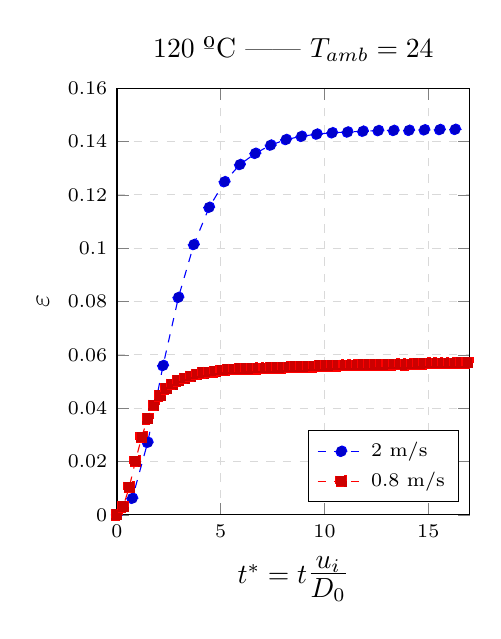
\begin{tikzpicture}
\begin{axis}[
	title = {120 ºC || $T_{amb}=24$},
    tick label style={font=\scriptsize},
    legend style={font=\scriptsize,/tikz/column 2/.style={column sep=5pt},},
    %legend columns=2,
    legend cell align=left,
	legend pos =south east,
    grid=major, % Display a grid
    grid style={dashed,gray!30}, % Set the style
    xlabel={$t^*=t$\Large{$\frac{u_i}{D_0}$}},
    ylabel={$\varepsilon$}, 
    ymin = 0, ymax = 0.16,
    ytick={0,0.02,0.04,0.06,0.08,0.1,0.12,0.14,0.16},
    yticklabels={0,0.02,0.04,0.06,0.08,0.1,0.12,0.14,0.16},
    xmin = 0, xmax = 17,
    %ytick={0,1600,...,11200},
    %yticklabel style={
    %    /pgf/number format/fixed,
    %    /pgf/number format/precision=5},
	%scaled y ticks=false,
    width=0.5\textwidth, 
    height=7cm,
    cycle list name= color
    ]
\addplot+[dashed]
coordinates {(	0	,	0	)
(	0.740740741	,	0.006204439	)
(	1.481481481	,	0.027167401	)
(	2.222222222	,	0.055996228	)
(	2.962962963	,	0.081552623	)
(	3.703703704	,	0.10136598	)
(	4.444444444	,	0.11532131	)
(	5.185185185	,	0.124927101	)
(	5.925925926	,	0.131361385	)
(	6.666666667	,	0.135565292	)
(	7.407407407	,	0.13864324	)
(	8.148148148	,	0.140741531	)
(	8.888888889	,	0.141945242	)
(	9.62962963	,	0.142768713	)
(	10.37037037	,	0.14327807	)
(	11.11111111	,	0.143565689	)
(	11.85185185	,	0.143854306	)
(	12.59259259	,	0.144099116	)
(	13.33333333	,	0.144154172	)
(	14.07407407	,	0.144202739	)
(	14.81481481	,	0.144379603	)
(	15.55555556	,	0.144484393	)
(	16.2962963	,	0.14455193	)
(	17.03703704	,	0.144595472	)
(	17.77777778	,	0.144529085	)
(	18.51851852	,	0.144559185	)
};
\addlegendentry{2 m/s}
\addplot+[dashed]
coordinates {(	0	,	0	)
(	0.296296296	,	0.003018616	)
(	0.592592593	,	0.010388567	)
(	0.888888889	,	0.020058751	)
(	1.185185185	,	0.029057225	)
(	1.481481481	,	0.036086665	)
(	1.777777778	,	0.041101457	)
(	2.074074074	,	0.044656137	)
(	2.37037037	,	0.047221941	)
(	2.666666667	,	0.04900349	)
(	2.962962963	,	0.050282037	)
(	3.259259259	,	0.051294611	)
(	3.555555556	,	0.052024343	)
(	3.851851852	,	0.052657377	)
(	4.148148148	,	0.053180309	)
(	4.444444444	,	0.053460793	)
(	4.740740741	,	0.053762748	)
(	5.037037037	,	0.05417938	)
(	5.333333333	,	0.054450507	)
(	5.62962963	,	0.054606891	)
(	5.925925926	,	0.05471092	)
(	6.222222222	,	0.054767125	)
(	6.518518519	,	0.054849489	)
(	6.814814815	,	0.054895029	)
(	7.111111111	,	0.054987799	)
(	7.407407407	,	0.055055601	)
(	7.703703704	,	0.055123722	)
(	8	,	0.055238927	)
(	8.296296296	,	0.055369558	)
(	8.592592593	,	0.055460231	)
(	8.888888889	,	0.055500837	)
(	9.185185185	,	0.055470796	)
(	9.481481481	,	0.055637519	)
(	9.777777778	,	0.055874762	)
(	10.07407407	,	0.05589608	)
(	10.37037037	,	0.05592535	)
(	10.66666667	,	0.05601879	)
(	10.96296296	,	0.056082886	)
(	11.25925926	,	0.056085747	)
(	11.55555556	,	0.05616628	)
(	11.85185185	,	0.05621398	)
(	12.14814815	,	0.056192707	)
(	12.44444444	,	0.056216044	)
(	12.74074074	,	0.05628988	)
(	13.03703704	,	0.056334466	)
(	13.33333333	,	0.056389648	)
(	13.62962963	,	0.056410617	)
(	13.92592593	,	0.056360938	)
(	14.22222222	,	0.056440896	)
(	14.51851852	,	0.056619325	)
(	14.81481481	,	0.056718913	)
(	15.11111111	,	0.056785331	)
(	15.40740741	,	0.056809146	)
(	15.7037037	,	0.056815796	)
(	16	,	0.056834251	)
(	16.2962963	,	0.0568721	)
(	16.59259259	,	0.056924773	)
(	16.88888889	,	0.05697371	)
(	17.18518519	,	0.057029045	)
(	17.48148148	,	0	)
};
\addlegendentry{0.8 m/s}
\end{axis}
\end{tikzpicture}}
\caption{Computed cooling effectiveness comparison between two different impact velocity values for the initial foil temperature of 120ºC}
\label{fig:speedcool}
\end{figure}

\par With these results it is possible to reaffirm what some previous authors studied. The impact velocity affects positively the cooling efficiency as the wetted area is bigger and convection heat transfer increases.\\

\subsection{Influence of the initial foil temperature}

\par This section will address the relative temperature drop in the foil for the tested temperatures. The temperatures had to be adimensionalised  so that they could be compared. This analysis, for a fixed impact velocity of 0.8 m/s, can be seen in Figure \ref{fig:temp}. In this figure one can see that for different initial temperatures, the relative temperature drop is very similar in the center region, but has a significant difference in the edge area. This may be due to the different spreading diameters at that time (larger input velocities lead to larger spreading diameters), which can shift the curve.\\

\begin{figure}[h]
\centering
\subfigure[3 ms]{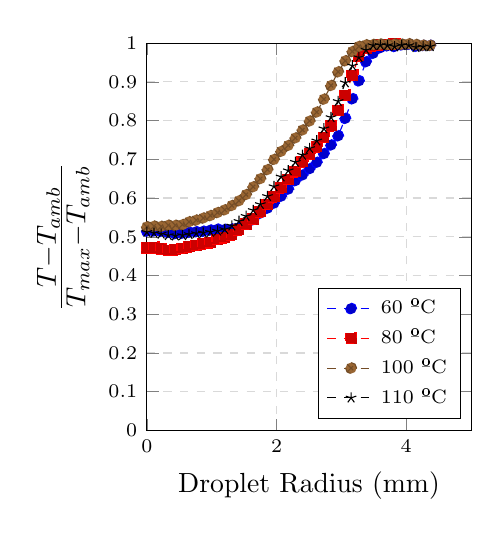
\begin{tikzpicture}
\begin{axis}[
	%title = {0.8 m/s || 3ms},
    tick label style={font=\scriptsize},
    legend style={font=\scriptsize,/tikz/column 2/.style={column sep=5pt},},
    %legend columns=2,
    legend cell align=left,
	legend pos =south east,
    grid=major, % Display a grid
    grid style={dashed,gray!30}, % Set the style
    xlabel={Droplet Radius (mm)},
    ylabel={\Large{$\frac{T-T_{amb}}{T_{max}-T_{amb}}$}}, 
    ymin = 0, ymax = 1,
    ytick={0,0.1,...,1},
    %yticklabels={300,325,350,375,400,425,450,475,500,525},
    xmin = 0, xmax = 5,
    %ytick={0,1600,...,11200},
    %yticklabel style={
    %    /pgf/number format/fixed,
    %    /pgf/number format/precision=5},
	%scaled y ticks=false,
    width=0.47\textwidth, 
    height=6.5cm,
    cycle list name= color
    ]
\addplot+[dashed]
coordinates {(	0	,	0.514798887	)
(	0.11	,	0.515304832	)
(	0.22	,	0.514292942	)
(	0.33	,	0.511257273	)
(	0.44	,	0.508221604	)
(	0.55	,	0.509233494	)
(	0.65	,	0.511510245	)
(	0.76	,	0.51302808	)
(	0.87	,	0.514292942	)
(	0.98	,	0.517328611	)
(	1.09	,	0.519605363	)
(	1.2	,	0.518846446	)
(	1.31	,	0.519858335	)
(	1.42	,	0.523652922	)
(	1.53	,	0.532506957	)
(	1.64	,	0.544143688	)
(	1.75	,	0.560839868	)
(	1.86	,	0.573741462	)
(	1.96	,	0.586643056	)
(	2.07	,	0.604604098	)
(	2.18	,	0.622818113	)
(	2.29	,	0.644826714	)
(	2.4	,	0.659499115	)
(	2.51	,	0.67568935	)
(	2.62	,	0.692132558	)
(	2.73	,	0.714647103	)
(	2.84	,	0.736908677	)
(	2.95	,	0.760688085	)
(	3.06	,	0.805717177	)
(	3.17	,	0.856311662	)
(	3.27	,	0.902605616	)
(	3.38	,	0.951935239	)
(	3.49	,	0.973690868	)
(	3.6	,	0.988110296	)
(	3.71	,	0.993169744	)
(	3.82	,	0.991398938	)
(	3.93	,	0.995446496	)
(	4.04	,	0.996964331	)
(	4.15	,	0.991904882	)
(	4.26	,	0.993928662	)
(	4.37	,	0.994181634	)
};
\addlegendentry{60 ºC}

\addplot+[dashed]
coordinates {(	0	,	0.471055243	)
(	0.11	,	0.472213033	)
(	0.22	,	0.469401257	)
(	0.33	,	0.465597089	)
(	0.44	,	0.466093285	)
(	0.55	,	0.470724446	)
(	0.65	,	0.474694013	)
(	0.76	,	0.478167383	)
(	0.87	,	0.481640754	)
(	0.98	,	0.485279524	)
(	1.09	,	0.493384056	)
(	1.2	,	0.498346014	)
(	1.31	,	0.504961958	)
(	1.42	,	0.518193847	)
(	1.53	,	0.532914324	)
(	1.64	,	0.545815415	)
(	1.75	,	0.564836255	)
(	1.86	,	0.583691697	)
(	1.96	,	0.603704929	)
(	2.07	,	0.626364539	)
(	2.18	,	0.648362554	)
(	2.29	,	0.668706583	)
(	2.4	,	0.69401257	)
(	2.51	,	0.713695005	)
(	2.62	,	0.733046642	)
(	2.73	,	0.756864042	)
(	2.84	,	0.786966589	)
(	2.95	,	0.826993053	)
(	3.06	,	0.865861727	)
(	3.17	,	0.916804499	)
(	3.27	,	0.967251075	)
(	3.38	,	0.986602713	)
(	3.49	,	0.993549454	)
(	3.6	,	0.995699636	)
(	3.71	,	0.997519021	)
(	3.82	,	0.998346014	)
};
\addlegendentry{80 ºC}

\addplot+[dashed]
coordinates {(	0	,	0.525613593	)
(	0.11	,	0.527375708	)
(	0.22	,	0.526746381	)
(	0.33	,	0.529767149	)
(	0.44	,	0.529515419	)
(	0.55	,	0.531403398	)
(	0.65	,	0.538577722	)
(	0.76	,	0.542983008	)
(	0.87	,	0.548395217	)
(	0.98	,	0.554688483	)
(	1.09	,	0.562492133	)
(	1.2	,	0.569540592	)
(	1.31	,	0.580742605	)
(	1.42	,	0.592951542	)
(	1.53	,	0.608936438	)
(	1.64	,	0.62907489	)
(	1.75	,	0.649968534	)
(	1.86	,	0.673379484	)
(	1.96	,	0.699811202	)
(	2.07	,	0.72057898	)
(	2.18	,	0.735808685	)
(	2.29	,	0.755191945	)
(	2.4	,	0.775707992	)
(	2.51	,	0.798867212	)
(	2.62	,	0.822026432	)
(	2.73	,	0.855380743	)
(	2.84	,	0.890623033	)
(	2.95	,	0.925865324	)
(	3.06	,	0.954436753	)
(	3.17	,	0.97847703	)
(	3.27	,	0.991567023	)
(	3.38	,	0.995468848	)
(	3.49	,	0.996475771	)
(	3.6	,	0.997482694	)
(	3.71	,	0.99597231	)
(	3.82	,	0.997230963	)
(	3.93	,	0.997105098	)
(	4.04	,	0.998237885	)
(	4.15	,	0.996475771	)
(	4.26	,	0.994587791	)
(	4.37	,	0.994210195	)
};
\addlegendentry{100 ºC}

\addplot+[dashed]
coordinates {(	0	,	0.511852408	)
(	0.11	,	0.509385391	)
(	0.22	,	0.507240159	)
(	0.33	,	0.503486002	)
(	0.44	,	0.502520648	)
(	0.55	,	0.503593264	)
(	0.65	,	0.506274804	)
(	0.76	,	0.50863456	)
(	0.87	,	0.510243484	)
(	0.98	,	0.512174193	)
(	1.09	,	0.515070256	)
(	1.2	,	0.519146198	)
(	1.31	,	0.528156173	)
(	1.42	,	0.540062212	)
(	1.53	,	0.553148128	)
(	1.64	,	0.568379277	)
(	1.75	,	0.583717687	)
(	1.86	,	0.60452644	)
(	1.96	,	0.62984018	)
(	2.07	,	0.654939397	)
(	2.18	,	0.670921377	)
(	2.29	,	0.692802746	)
(	2.4	,	0.710929958	)
(	2.51	,	0.728199078	)
(	2.62	,	0.747935214	)
(	2.73	,	0.779255604	)
(	2.84	,	0.808216239	)
(	2.95	,	0.849833745	)
(	3.06	,	0.897886946	)
(	3.17	,	0.941649684	)
(	3.27	,	0.962994744	)
(	3.38	,	0.981980049	)
(	3.49	,	0.99399335	)
(	3.6	,	0.994529658	)
(	3.71	,	0.994100611	)
(	3.82	,	0.990882763	)
(	3.93	,	0.994529658	)
(	4.04	,	0.994100611	)
(	4.15	,	0.989059316	)
(	4.26	,	0.990775501	)
(	4.37	,	0.99131181	)
};
\addlegendentry{110 ºC}

\end{axis}
\end{tikzpicture}}
\subfigure[13 ms]{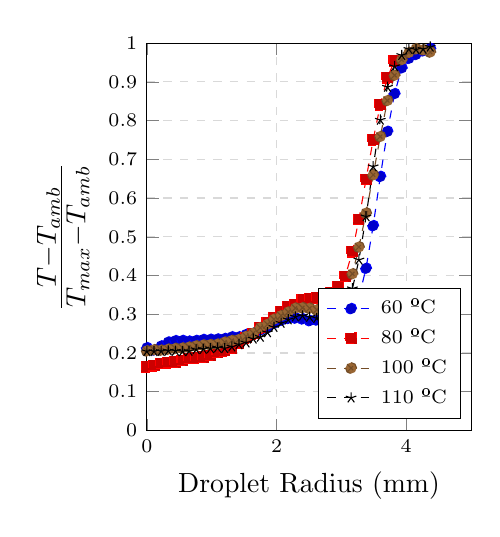
\begin{tikzpicture}
\begin{axis}[
	%title = {0.8 m/s || 13ms},
    tick label style={font=\scriptsize},
    legend style={font=\scriptsize,/tikz/column 2/.style={column sep=5pt},},
    %legend columns=2,
    legend cell align=left,
	legend pos =south east,
    grid=major, % Display a grid
    grid style={dashed,gray!30}, % Set the style
    xlabel={Droplet Radius (mm)},
    ylabel={\Large{$\frac{T-T_{amb}}{T_{max}-T_{amb}}$}}, 
    ymin = 0, ymax = 1,
    ytick={0,0.1,...,1},
    %yticklabels={300,325,350,375,400,425,450,475,500,525},
    xmin = 0, xmax = 5,
    %ytick={0,1600,...,11200},
    %yticklabel style={
    %    /pgf/number format/fixed,
    %    /pgf/number format/precision=5},
	%scaled y ticks=false,
    width=0.47\textwidth, 
    height=6.5cm,
    cycle list name= color
    ]
\addplot+[dashed]
coordinates {(	0	,	0.213508728	)
(	0.11	,	0.207690362	)
(	0.22	,	0.218062231	)
(	0.33	,	0.228181128	)
(	0.44	,	0.231722742	)
(	0.55	,	0.232228687	)
(	0.65	,	0.23045788	)
(	0.76	,	0.232228687	)
(	0.87	,	0.234758411	)
(	0.98	,	0.235264356	)
(	1.09	,	0.236023273	)
(	1.2	,	0.237288136	)
(	1.31	,	0.241588667	)
(	1.42	,	0.241588667	)
(	1.53	,	0.247912977	)
(	1.64	,	0.250948647	)
(	1.75	,	0.259296737	)
(	1.86	,	0.26486213	)
(	1.96	,	0.276498862	)
(	2.07	,	0.284341007	)
(	2.18	,	0.289147483	)
(	2.29	,	0.290159373	)
(	2.4	,	0.287882621	)
(	2.51	,	0.283329117	)
(	2.62	,	0.285099924	)
(	2.73	,	0.280799393	)
(	2.84	,	0.277004806	)
(	2.95	,	0.277004806	)
(	3.06	,	0.285352897	)
(	3.17	,	0.300025297	)
(	3.27	,	0.343283582	)
(	3.38	,	0.418669365	)
(	3.49	,	0.52871237	)
(	3.6	,	0.655704528	)
(	3.71	,	0.772071844	)
(	3.82	,	0.869466228	)
(	3.93	,	0.935997976	)
(	4.04	,	0.960536302	)
(	4.15	,	0.970655199	)
(	4.26	,	0.980015178	)
(	4.37	,	0.986086517	)
};
\addlegendentry{60 ºC}

\addplot+[dashed]
coordinates {(	0	,	0.163910023	)
(	0.11	,	0.167714191	)
(	0.22	,	0.173337744	)
(	0.33	,	0.175487926	)
(	0.44	,	0.176645716	)
(	0.55	,	0.180780681	)
(	0.65	,	0.186073437	)
(	0.76	,	0.187231227	)
(	0.87	,	0.189546808	)
(	0.98	,	0.194177969	)
(	1.09	,	0.201786305	)
(	1.2	,	0.206086669	)
(	1.31	,	0.212537215	)
(	1.42	,	0.225107509	)
(	1.53	,	0.239000992	)
(	1.64	,	0.249090308	)
(	1.75	,	0.264803176	)
(	1.86	,	0.279689051	)
(	1.96	,	0.292590142	)
(	2.07	,	0.306152828	)
(	2.18	,	0.318888521	)
(	2.29	,	0.32500827	)
(	2.4	,	0.336751571	)
(	2.51	,	0.340886537	)
(	2.62	,	0.342044327	)
(	2.73	,	0.348329474	)
(	2.84	,	0.35593781	)
(	2.95	,	0.37148528	)
(	3.06	,	0.398445253	)
(	3.17	,	0.462123718	)
(	3.27	,	0.545650017	)
(	3.38	,	0.648197155	)
(	3.49	,	0.750909692	)
(	3.6	,	0.840555739	)
(	3.71	,	0.911346345	)
(	3.82	,	0.954515382	)
};
\addlegendentry{80 ºC}

\addplot+[dashed]
coordinates {(	0	,	0.205286344	)
(	0.11	,	0.208307111	)
(	0.22	,	0.207174323	)
(	0.33	,	0.209817495	)
(	0.44	,	0.211705475	)
(	0.55	,	0.212838263	)
(	0.65	,	0.215229704	)
(	0.76	,	0.218502203	)
(	0.87	,	0.220516048	)
(	0.98	,	0.22152297	)
(	1.09	,	0.222907489	)
(	1.2	,	0.228067967	)
(	1.31	,	0.232221523	)
(	1.42	,	0.234864695	)
(	1.53	,	0.243045941	)
(	1.64	,	0.251101322	)
(	1.75	,	0.265198238	)
(	1.86	,	0.274008811	)
(	1.96	,	0.287098804	)
(	2.07	,	0.296286973	)
(	2.18	,	0.305726872	)
(	2.29	,	0.315796098	)
(	2.4	,	0.316803021	)
(	2.51	,	0.315292637	)
(	2.62	,	0.311516677	)
(	2.73	,	0.305726872	)
(	2.84	,	0.309628697	)
(	2.95	,	0.320956576	)
(	3.06	,	0.34751416	)
(	3.17	,	0.404405286	)
(	3.27	,	0.473631215	)
(	3.38	,	0.56123348	)
(	3.49	,	0.659786029	)
(	3.6	,	0.758842039	)
(	3.71	,	0.851730648	)
(	3.82	,	0.916803021	)
(	3.93	,	0.95720579	)
(	4.04	,	0.975833858	)
(	4.15	,	0.985273757	)
(	4.26	,	0.982756451	)
(	4.37	,	0.976966646	)
};
\addlegendentry{100 ºC}

\addplot+[dashed]
coordinates {(	0	,	0.203797061	)
(	0.11	,	0.203904323	)
(	0.22	,	0.204226107	)
(	0.33	,	0.205513247	)
(	0.44	,	0.204976939	)
(	0.55	,	0.203904323	)
(	0.65	,	0.204440631	)
(	0.76	,	0.208945618	)
(	0.87	,	0.209803711	)
(	0.98	,	0.211519897	)
(	1.09	,	0.213343344	)
(	1.2	,	0.211412635	)
(	1.31	,	0.2157031	)
(	1.42	,	0.221495227	)
(	1.53	,	0.226107476	)
(	1.64	,	0.236190068	)
(	1.75	,	0.240909578	)
(	1.86	,	0.252708356	)
(	1.96	,	0.26633058	)
(	2.07	,	0.277056741	)
(	2.18	,	0.285852193	)
(	2.29	,	0.293253245	)
(	2.4	,	0.295934785	)
(	2.51	,	0.292502413	)
(	2.62	,	0.289499088	)
(	2.73	,	0.28692481	)
(	2.84	,	0.285101362	)
(	2.95	,	0.298401802	)
(	3.06	,	0.31888877	)
(	3.17	,	0.36619114	)
(	3.27	,	0.440416175	)
(	3.38	,	0.551968251	)
(	3.49	,	0.68111123	)
(	3.6	,	0.801458758	)
(	3.71	,	0.886517215	)
(	3.82	,	0.939611713	)
(	3.93	,	0.968572348	)
(	4.04	,	0.984232543	)
(	4.15	,	0.983159927	)
(	4.26	,	0.984554328	)
(	4.37	,	0.99002467	)
};
\addlegendentry{110 ºC}

\end{axis}
\end{tikzpicture}}
\subfigure[23 ms]{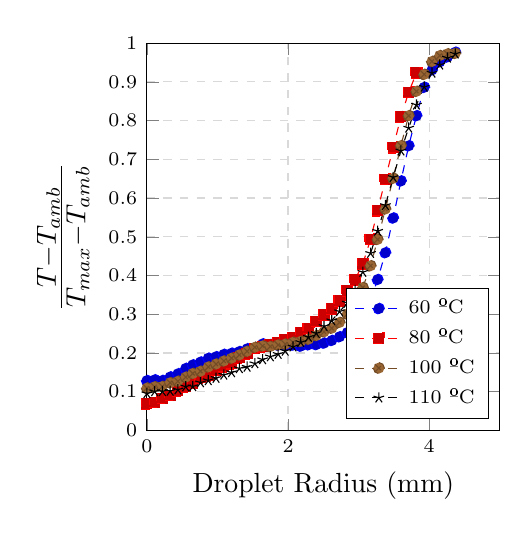
\begin{tikzpicture}
\begin{axis}[
	%title = {0.8 m/s || 23ms},
    tick label style={font=\scriptsize},
    legend style={font=\scriptsize,/tikz/column 2/.style={column sep=5pt},},
    %legend columns=2,
    legend cell align=left,
	legend pos =south east,
    grid=major, % Display a grid
    grid style={dashed,gray!30}, % Set the style
    xlabel={Droplet Radius (mm)},
    ylabel={\Large{$\frac{T-T_{amb}}{T_{max}-T_{amb}}$}}, 
    ymin = 0, ymax = 1,
    ytick={0,0.1,...,1},
    %yticklabels={300,325,350,375,400,425,450,475,500,525},
    xmin = 0, xmax = 5,
    %ytick={0,1600,...,11200},
    %yticklabel style={
    %    /pgf/number format/fixed,
    %    /pgf/number format/precision=5},
	%scaled y ticks=false,
    width=0.5\textwidth, 
    height=6.5cm,
    cycle list name= color
    ]
\addplot+[dashed]
coordinates {(	0	,	0.128509992	)
(	0.11	,	0.130533772	)
(	0.22	,	0.129015937	)
(	0.33	,	0.138122945	)
(	0.44	,	0.146218062	)
(	0.55	,	0.160131546	)
(	0.65	,	0.169238553	)
(	0.76	,	0.176574753	)
(	0.87	,	0.186440678	)
(	0.98	,	0.190235264	)
(	1.09	,	0.196306603	)
(	1.2	,	0.199342272	)
(	1.31	,	0.203642803	)
(	1.42	,	0.210726031	)
(	1.53	,	0.2137617	)
(	1.64	,	0.223374652	)
(	1.75	,	0.221603845	)
(	1.86	,	0.220086011	)
(	1.96	,	0.219833038	)
(	2.07	,	0.220338983	)
(	2.18	,	0.217556286	)
(	2.29	,	0.2210979	)
(	2.4	,	0.221603845	)
(	2.51	,	0.225398432	)
(	2.62	,	0.232228687	)
(	2.73	,	0.241841639	)
(	2.84	,	0.252719454	)
(	2.95	,	0.269162661	)
(	3.06	,	0.297495573	)
(	3.17	,	0.337465216	)
(	3.27	,	0.389577536	)
(	3.38	,	0.458891981	)
(	3.49	,	0.54844422	)
(	3.6	,	0.644067797	)
(	3.71	,	0.734884898	)
(	3.82	,	0.812547432	)
(	3.93	,	0.885909436	)
(	4.04	,	0.930685555	)
(	4.15	,	0.951429294	)
(	4.26	,	0.964330888	)
(	4.37	,	0.976473564	)
};
\addlegendentry{60 ºC}

\addplot+[dashed]
coordinates {(	0	,	0.068640423	)
(	0.11	,	0.072940787	)
(	0.22	,	0.083195501	)
(	0.33	,	0.091300033	)
(	0.44	,	0.10238174	)
(	0.55	,	0.112801852	)
(	0.65	,	0.122394972	)
(	0.76	,	0.135461462	)
(	0.87	,	0.141581211	)
(	0.98	,	0.155805491	)
(	1.09	,	0.165233212	)
(	1.2	,	0.173006947	)
(	1.31	,	0.187231227	)
(	1.42	,	0.197982137	)
(	1.53	,	0.21187562	)
(	1.64	,	0.216837579	)
(	1.75	,	0.221799537	)
(	1.86	,	0.226265299	)
(	1.96	,	0.233873635	)
(	2.07	,	0.240324181	)
(	2.18	,	0.253225273	)
(	2.29	,	0.26430698	)
(	2.4	,	0.281508435	)
(	2.51	,	0.298048296	)
(	2.62	,	0.313430367	)
(	2.73	,	0.334105194	)
(	2.84	,	0.359907377	)
(	2.95	,	0.389017532	)
(	3.06	,	0.430532584	)
(	3.17	,	0.493549454	)
(	3.27	,	0.567978829	)
(	3.38	,	0.649024148	)
(	3.49	,	0.730731062	)
(	3.6	,	0.809626199	)
(	3.71	,	0.873139266	)
(	3.82	,	0.922924247	)
};
\addlegendentry{80 ºC}

\addplot+[dashed]
coordinates {(	0	,	0.109251101	)
(	0.11	,	0.112649465	)
(	0.22	,	0.113530522	)
(	0.33	,	0.122970422	)
(	0.44	,	0.126998112	)
(	0.55	,	0.137570799	)
(	0.65	,	0.147010699	)
(	0.76	,	0.152800503	)
(	0.87	,	0.163876652	)
(	0.98	,	0.171428571	)
(	1.09	,	0.179232222	)
(	1.2	,	0.18653241	)
(	1.31	,	0.194965387	)
(	1.42	,	0.204279421	)
(	1.53	,	0.214600378	)
(	1.64	,	0.218124607	)
(	1.75	,	0.216614223	)
(	1.86	,	0.220767778	)
(	1.96	,	0.222781624	)
(	2.07	,	0.227438641	)
(	2.18	,	0.229955947	)
(	2.29	,	0.235494021	)
(	2.4	,	0.244933921	)
(	2.51	,	0.254499685	)
(	2.62	,	0.263813719	)
(	2.73	,	0.278791693	)
(	2.84	,	0.300692259	)
(	2.95	,	0.328005035	)
(	3.06	,	0.368911265	)
(	3.17	,	0.425173065	)
(	3.27	,	0.49314034	)
(	3.38	,	0.571680302	)
(	3.49	,	0.650849591	)
(	3.6	,	0.735305223	)
(	3.71	,	0.812712398	)
(	3.82	,	0.875519194	)
(	3.93	,	0.919320327	)
(	4.04	,	0.952674638	)
(	4.15	,	0.967778477	)
(	4.26	,	0.972435494	)
(	4.37	,	0.973442417	)
};
\addlegendentry{100 ºC}

\addplot+[dashed]
coordinates {(	0	,	0.095248311	)
(	0.11	,	0.100396868	)
(	0.22	,	0.100611391	)
(	0.33	,	0.101576746	)
(	0.44	,	0.105009117	)
(	0.55	,	0.112839215	)
(	0.65	,	0.113268261	)
(	0.76	,	0.123350853	)
(	0.87	,	0.128821195	)
(	0.98	,	0.134827845	)
(	1.09	,	0.143194251	)
(	1.2	,	0.149415424	)
(	1.31	,	0.159927062	)
(	1.42	,	0.163681218	)
(	1.53	,	0.172583932	)
(	1.64	,	0.182988308	)
(	1.75	,	0.19038936	)
(	1.86	,	0.196825056	)
(	1.96	,	0.204869677	)
(	2.07	,	0.215917623	)
(	2.18	,	0.227394615	)
(	2.29	,	0.240695055	)
(	2.4	,	0.250670385	)
(	2.51	,	0.268690336	)
(	2.62	,	0.283492438	)
(	2.73	,	0.306982731	)
(	2.84	,	0.329078623	)
(	2.95	,	0.361257106	)
(	3.06	,	0.408666738	)
(	3.17	,	0.457470771	)
(	3.27	,	0.51464121	)
(	3.38	,	0.581036147	)
(	3.49	,	0.653544996	)
(	3.6	,	0.721870642	)
(	3.71	,	0.78097179	)
(	3.82	,	0.840394723	)
(	3.93	,	0.886731739	)
(	4.04	,	0.922878902	)
(	4.15	,	0.943794916	)
(	4.26	,	0.961707605	)
(	4.37	,	0.972111981	)
};
\addlegendentry{110 ºC}

\end{axis}
\end{tikzpicture}}
\caption{Average adimensional temperature along the radius for 4 different initial temperatures at 0.8 m/s}
\label{fig:temp}
\end{figure}

\par This is a confirmation for the effectiveness of the  weighted background test. Because there is little variation between the adimensionalised temperature maps, one may argue that the relative variation of the temperature is similar. This legitimizes the use of the weighted background removal as a mean to obtain a uniform initial temperature.\\

\par To infer if the initial foil temperature has a relevant effect on the cooling effectiveness, one needs to plot several this parameter for several temperatures at the same impact velocity. These results are depicted Figure \ref{fig:tempcool} and \ref{fig:tempcool2}. In Figure \ref{fig:tempcool} it's clear that all curves are close to be coincident so, the initial temperature doesn't influence the cooling effectiveness. But one needs to be careful making this statement because, for 2 m/s, in Figure \ref{fig:tempcool2}, it's noticeable that the 110ºC curve is not close to the others, but instead is converging to a higher cooling effectiveness. This is due to phase change of the liquid which occurs during spreading, as the lamella's thickness is thinner at $u_i=2 m/s$, so boiling may occur within this thin lamela.\\

\begin{figure}[h!]
\centering
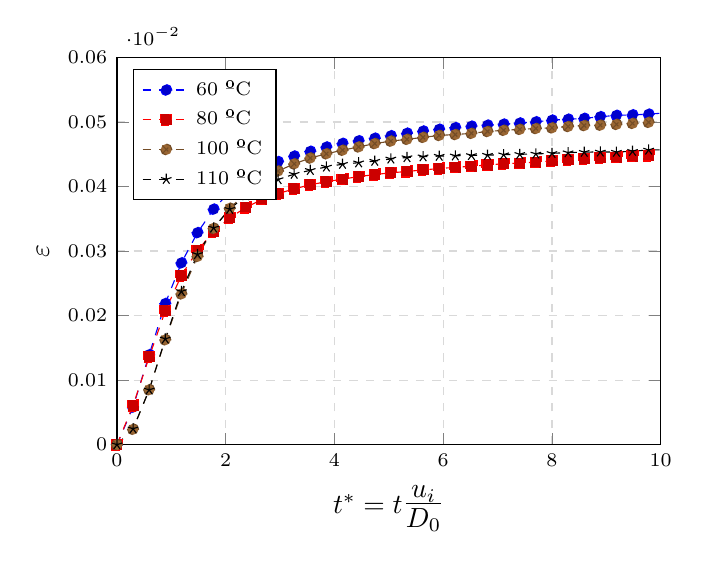
\begin{tikzpicture}
\begin{axis}[
	%title = {0.8 m/s || $T_{amb}=24$},
    tick label style={font=\scriptsize},
    legend style={font=\scriptsize,/tikz/column 2/.style={column sep=5pt},},
    %legend columns=2,
    legend cell align=left,
	legend pos =north west,
    grid=major, % Display a grid
    grid style={dashed,gray!30}, % Set the style
    xlabel={$t^*=t$\Large{$\frac{u_i}{D_0}$}},
    ylabel={$\varepsilon$}, 
    ymin = 0, ymax = 0.06,
    ytick={0,0.01,0.02,0.03,0.04,0.05,0.06},
    yticklabels={0,0.01,0.02,0.03,0.04,0.05,0.06},
    xmin = 0, xmax = 10,
    %ytick={0,1600,...,11200},
    %yticklabel style={
    %    /pgf/number format/fixed,
    %    /pgf/number format/precision=5},
	%scaled y ticks=false,
    width=0.7\textwidth, 
    height=6.5cm,
    cycle list name= color
    ]
\addplot+[dashed]
coordinates {(	0	,	0	)
(	0.296296296	,	0.005814028	)
(	0.592592593	,	0.013939001	)
(	0.888888889	,	0.021877251	)
(	1.185185185	,	0.02817158	)
(	1.481481481	,	0.032850495	)
(	1.777777778	,	0.036491362	)
(	2.074074074	,	0.039219849	)
(	2.37037037	,	0.04118402	)
(	2.666666667	,	0.042720846	)
(	2.962962963	,	0.043846373	)
(	3.259259259	,	0.044713117	)
(	3.555555556	,	0.04545311	)
(	3.851851852	,	0.046115677	)
(	4.148148148	,	0.046678768	)
(	4.444444444	,	0.047083448	)
(	4.740740741	,	0.047480854	)
(	5.037037037	,	0.047861223	)
(	5.333333333	,	0.048256869	)
(	5.62962963	,	0.048592487	)
(	5.925925926	,	0.048867444	)
(	6.222222222	,	0.049117083	)
(	6.518518519	,	0.049342712	)
(	6.814814815	,	0.049504816	)
(	7.111111111	,	0.049661762	)
(	7.407407407	,	0.049835518	)
(	7.703703704	,	0.050020441	)
(	8	,	0.050278806	)
(	8.296296296	,	0.050424933	)
(	8.592592593	,	0.050554038	)
(	8.888888889	,	0.050814487	)
(	9.185185185	,	0.051019483	)
(	9.481481481	,	0.051103522	)
(	9.777777778	,	0.051200508	)
(	10.07407407	,	0.051407132	)
(	10.37037037	,	0.05158612	)
(	10.66666667	,	0.051641101	)
(	10.96296296	,	0.051758566	)
(	11.25925926	,	0.051982552	)
(	11.55555556	,	0.052132765	)
(	11.85185185	,	0.052249029	)
(	12.14814815	,	0.052417982	)
(	12.44444444	,	0.052557033	)
(	12.74074074	,	0.052634441	)
(	13.03703704	,	0.052686625	)
(	13.33333333	,	0.052847845	)
(	13.62962963	,	0.052991337	)
(	13.92592593	,	0.053109366	)
(	14.22222222	,	0.053256169	)
(	14.51851852	,	0.053342202	)
(	14.81481481	,	0.053424223	)
(	15.11111111	,	0.053565347	)
(	15.40740741	,	0.053717764	)
(	15.7037037	,	0.053816081	)
(	16	,	0.053843081	)
(	16.2962963	,	0.053905726	)
(	16.59259259	,	0.054018883	)
(	16.88888889	,	0.05413619	)
(	17.18518519	,	0.054234201	)
};
\addlegendentry{60 ºC}
\addplot+[dashed]
coordinates {(	0	,	0	)
(	0.296296296	,	0.006063781	)
(	0.592592593	,	0.013591181	)
(	0.888888889	,	0.020738029	)
(	1.185185185	,	0.026206704	)
(	1.481481481	,	0.030101381	)
(	1.777777778	,	0.033000256	)
(	2.074074074	,	0.035149834	)
(	2.37037037	,	0.036744509	)
(	2.666666667	,	0.038001938	)
(	2.962962963	,	0.038901639	)
(	3.259259259	,	0.039629625	)
(	3.555555556	,	0.040273734	)
(	3.851851852	,	0.040745884	)
(	4.148148148	,	0.04115001	)
(	4.444444444	,	0.041527058	)
(	4.740740741	,	0.041854521	)
(	5.037037037	,	0.042117494	)
(	5.333333333	,	0.042332715	)
(	5.62962963	,	0.042562776	)
(	5.925925926	,	0.042786403	)
(	6.222222222	,	0.042968476	)
(	6.518518519	,	0.043142198	)
(	6.814814815	,	0.043335791	)
(	7.111111111	,	0.043527484	)
(	7.407407407	,	0.043633356	)
(	7.703703704	,	0.043767519	)
(	8	,	0.043960686	)
(	8.296296296	,	0.044120191	)
(	8.592592593	,	0.044318135	)
(	8.888888889	,	0.044455583	)
(	9.185185185	,	0.044564726	)
(	9.481481481	,	0.044726978	)
(	9.777777778	,	0.044815744	)
(	10.07407407	,	0.044910609	)
(	10.37037037	,	0.045040888	)
(	10.66666667	,	0.045115525	)
(	10.96296296	,	0.045189647	)
(	11.25925926	,	0.045277548	)
(	11.55555556	,	0.045361608	)
(	11.85185185	,	0.045410201	)
(	12.14814815	,	0.045501144	)
(	12.44444444	,	0.045613103	)
(	12.74074074	,	0.045722218	)
(	13.03703704	,	0.045814126	)
(	13.33333333	,	0.045903789	)
(	13.62962963	,	0.046072813	)
(	13.92592593	,	0.046106297	)
(	14.22222222	,	0.046127773	)
(	14.51851852	,	0.046283139	)
(	14.81481481	,	0.046427454	)
(	15.11111111	,	0.046509016	)
(	15.40740741	,	0.046578791	)
(	15.7037037	,	0.04667881	)
(	16	,	0.046729628	)
(	16.2962963	,	0.046814451	)
(	16.59259259	,	0.046910689	)
(	16.88888889	,	0.046935019	)
(	17.18518519	,	0.046999754	)
};
\addlegendentry{80 ºC}
\addplot+[dashed]
coordinates {(	0	,	0	)
(	0.296296296	,	0.002392246	)
(	0.592592593	,	0.008517691	)
(	0.888888889	,	0.016252305	)
(	1.185185185	,	0.023363829	)
(	1.481481481	,	0.029164598	)
(	1.777777778	,	0.033525029	)
(	2.074074074	,	0.036626678	)
(	2.37037037	,	0.038992699	)
(	2.666666667	,	0.040953332	)
(	2.962962963	,	0.042394543	)
(	3.259259259	,	0.043506583	)
(	3.555555556	,	0.044412609	)
(	3.851851852	,	0.045072766	)
(	4.148148148	,	0.045620248	)
(	4.444444444	,	0.046134789	)
(	4.740740741	,	0.046649117	)
(	5.037037037	,	0.047034179	)
(	5.333333333	,	0.04730966	)
(	5.62962963	,	0.047612949	)
(	5.925925926	,	0.047914865	)
(	6.222222222	,	0.048052598	)
(	6.518518519	,	0.048236655	)
(	6.814814815	,	0.048522984	)
(	7.111111111	,	0.048707994	)
(	7.407407407	,	0.048850561	)
(	7.703703704	,	0.048981771	)
(	8	,	0.049087216	)
(	8.296296296	,	0.049299104	)
(	8.592592593	,	0.049442034	)
(	8.888888889	,	0.049504048	)
(	9.185185185	,	0.049623276	)
(	9.481481481	,	0.049784724	)
(	9.777777778	,	0.049941762	)
(	10.07407407	,	0.050010965	)
(	10.37037037	,	0.05012469	)
(	10.66666667	,	0.050223548	)
(	10.96296296	,	0.050295124	)
(	11.25925926	,	0.050391813	)
(	11.55555556	,	0.050469145	)
(	11.85185185	,	0.050537405	)
(	12.14814815	,	0.050605087	)
(	12.44444444	,	0.050666561	)
(	12.74074074	,	0.050768001	)
(	13.03703704	,	0.050901498	)
(	13.33333333	,	0.051004327	)
(	13.62962963	,	0.051113224	)
(	13.92592593	,	0.051232699	)
(	14.22222222	,	0.051387127	)
(	14.51851852	,	0.051467752	)
(	14.81481481	,	0.05149836	)
(	15.11111111	,	0.051625585	)
(	15.40740741	,	0.051723859	)
(	15.7037037	,	0.051766522	)
(	16	,	0.051792484	)
(	16.2962963	,	0.0518612	)
(	16.59259259	,	0.052008733	)
(	16.88888889	,	0.052079051	)
(	17.18518519	,	0.052132412	)
};
\addlegendentry{100 ºC}
\addplot+[dashed]
coordinates {(	0	,	0	)
(	0.296296296	,	0.002466826	)
(	0.592592593	,	0.008489581	)
(	0.888888889	,	0.016392098	)
(	1.185185185	,	0.023745689	)
(	1.481481481	,	0.029490178	)
(	1.777777778	,	0.033588287	)
(	2.074074074	,	0.036493187	)
(	2.37037037	,	0.038589973	)
(	2.666666667	,	0.040045863	)
(	2.962962963	,	0.041090697	)
(	3.259259259	,	0.041918177	)
(	3.555555556	,	0.042514517	)
(	3.851851852	,	0.043031835	)
(	4.148148148	,	0.043459177	)
(	4.444444444	,	0.04368839	)
(	4.740740741	,	0.043935149	)
(	5.037037037	,	0.044275622	)
(	5.333333333	,	0.044497188	)
(	5.62962963	,	0.044624986	)
(	5.925925926	,	0.044709999	)
(	6.222222222	,	0.04475593	)
(	6.518518519	,	0.044823239	)
(	6.814814815	,	0.044860453	)
(	7.111111111	,	0.044936266	)
(	7.407407407	,	0.044991674	)
(	7.703703704	,	0.045047343	)
(	8	,	0.045141489	)
(	8.296296296	,	0.045248241	)
(	8.592592593	,	0.045322339	)
(	8.888888889	,	0.045355523	)
(	9.185185185	,	0.045330973	)
(	9.481481481	,	0.04546722	)
(	9.777777778	,	0.045661096	)
(	10.07407407	,	0.045678517	)
(	10.37037037	,	0.045702436	)
(	10.66666667	,	0.045778796	)
(	10.96296296	,	0.045831175	)
(	11.25925926	,	0.045833514	)
(	11.55555556	,	0.045899325	)
(	11.85185185	,	0.045938306	)
(	12.14814815	,	0.045920922	)
(	12.44444444	,	0.045939993	)
(	12.74074074	,	0.046000332	)
(	13.03703704	,	0.046036768	)
(	13.33333333	,	0.046081863	)
(	13.62962963	,	0.046098999	)
(	13.92592593	,	0.046058401	)
(	14.22222222	,	0.046123743	)
(	14.51851852	,	0.046269556	)
(	14.81481481	,	0.04635094	)
(	15.11111111	,	0.046405217	)
(	15.40740741	,	0.046424679	)
(	15.7037037	,	0.046430113	)
(	16	,	0.046445195	)
(	16.2962963	,	0.046476124	)
(	16.59259259	,	0.046519169	)
(	16.88888889	,	0.046559161	)
(	17.18518519	,	0.046604381	)
};
\addlegendentry{110 ºC}
\end{axis}
\end{tikzpicture}
\caption{Cooling effectiveness for various initial foil temperatures with an impact speed of 0.8 m/s}
\label{fig:tempcool}
\end{figure}

\begin{figure}[h!]
\centering
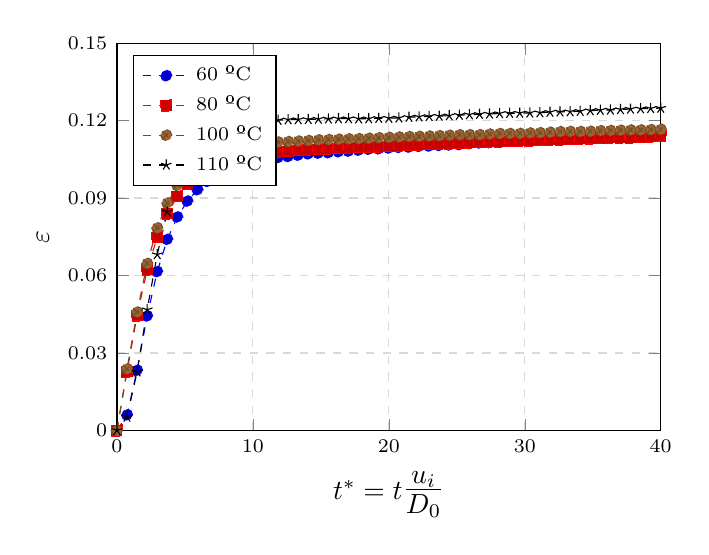
\begin{tikzpicture}
\begin{axis}[
	%title = {0.8 m/s || $T_{amb}=24$},
    tick label style={font=\scriptsize},
    legend style={font=\scriptsize,/tikz/column 2/.style={column sep=5pt},},
    %legend columns=2,
    legend cell align=left,
	legend pos =north west,
    grid=major, % Display a grid
    grid style={dashed,gray!30}, % Set the style
    xlabel={$t^*=t$\Large{$\frac{u_i}{D_0}$}},
    ylabel={$\varepsilon$}, 
    ymin = 0, ymax = 0.15,
    ytick={0,0.03,0.06,0.09,0.12,0.15},
    yticklabels={0,0.03,0.06,0.09,0.12,0.15},
    xmin = 0, xmax = 40,
    %ytick={0,1600,...,11200},
    %yticklabel style={
    %    /pgf/number format/fixed,
    %    /pgf/number format/precision=5},
	%scaled y ticks=false,
    width=0.7\textwidth, 
    height=6.5cm,
    cycle list name= color
    ]
\addplot+[dashed]
coordinates {(	0	,	0	)
(	0.740740741	,	0.006035623	)
(	1.481481481	,	0.023296885	)
(	2.222222222	,	0.044324934	)
(	2.962962963	,	0.061516245	)
(	3.703703704	,	0.074026746	)
(	4.444444444	,	0.08266424	)
(	5.185185185	,	0.088823023	)
(	5.925925926	,	0.093215682	)
(	6.666666667	,	0.0964551	)
(	7.407407407	,	0.098950056	)
(	8.148148148	,	0.100873508	)
(	8.888888889	,	0.102284517	)
(	9.62962963	,	0.103306453	)
(	10.37037037	,	0.104312171	)
(	11.11111111	,	0.105202546	)
(	11.85185185	,	0.105655176	)
(	12.59259259	,	0.106083205	)
(	13.33333333	,	0.106602158	)
(	14.07407407	,	0.107105012	)
(	14.81481481	,	0.107383638	)
(	15.55555556	,	0.107566074	)
(	16.2962963	,	0.107935361	)
(	17.03703704	,	0.108184641	)
(	17.77777778	,	0.108527665	)
(	18.51851852	,	0.108899146	)
(	19.25925926	,	0.109067316	)
(	20	,	0.109362957	)
(	20.74074074	,	0.109616074	)
(	21.48148148	,	0.109741722	)
(	22.22222222	,	0.110013716	)
(	22.96296296	,	0.110157966	)
(	23.7037037	,	0.110369338	)
(	24.44444444	,	0.110553385	)
(	25.18518519	,	0.11069292	)
(	25.92592593	,	0.111070696	)
(	26.66666667	,	0.111332461	)
(	27.40740741	,	0.111439259	)
(	28.14814815	,	0.111685778	)
(	28.88888889	,	0.111982219	)
(	29.62962963	,	0.112231578	)
(	30.37037037	,	0.112373565	)
(	31.11111111	,	0.112519609	)
(	31.85185185	,	0.112850086	)
(	32.59259259	,	0.113084671	)
(	33.33333333	,	0.113201572	)
(	34.07407407	,	0.113378997	)
(	34.81481481	,	0.113533717	)
(	35.55555556	,	0.113706924	)
(	36.2962963	,	0.11391115	)
(	37.03703704	,	0.114252631	)
(	37.77777778	,	0.114526895	)
(	38.51851852	,	0.114615593	)
(	39.25925926	,	0.114771614	)
(	40	,	0.114946243	)
(	40.74074074	,	0.115169445	)
(	41.48148148	,	0.115415108	)
(	42.22222222	,	0.115549593	)
(	42.96296296	,	0.115661083	)
};
\addlegendentry{60 ºC}
\addplot+[dashed]
coordinates {(	0	,	0	)
(	0.740740741	,	0.022654358	)
(	1.481481481	,	0.044543274	)
(	2.222222222	,	0.062264337	)
(	2.962962963	,	0.074882128	)
(	3.703703704	,	0.083936809	)
(	4.444444444	,	0.090640143	)
(	5.185185185	,	0.095443611	)
(	5.925925926	,	0.098849133	)
(	6.666666667	,	0.101411637	)
(	7.407407407	,	0.10325435	)
(	8.148148148	,	0.104533505	)
(	8.888888889	,	0.105524015	)
(	9.62962963	,	0.106400692	)
(	10.37037037	,	0.107032208	)
(	11.11111111	,	0.107579611	)
(	11.85185185	,	0.107944043	)
(	12.59259259	,	0.108201329	)
(	13.33333333	,	0.108521414	)
(	14.07407407	,	0.108769525	)
(	14.81481481	,	0.10896028	)
(	15.55555556	,	0.109096785	)
(	16.2962963	,	0.10928295	)
(	17.03703704	,	0.109503663	)
(	17.77777778	,	0.109672945	)
(	18.51851852	,	0.109761293	)
(	19.25925926	,	0.109863225	)
(	20	,	0.110005121	)
(	20.74074074	,	0.110227956	)
(	21.48148148	,	0.110452559	)
(	22.22222222	,	0.110609348	)
(	22.96296296	,	0.110815086	)
(	23.7037037	,	0.111038254	)
(	24.44444444	,	0.111109109	)
(	25.18518519	,	0.111222334	)
(	25.92592593	,	0.111476746	)
(	26.66666667	,	0.111646971	)
(	27.40740741	,	0.111727058	)
(	28.14814815	,	0.111811218	)
(	28.88888889	,	0.111988353	)
(	29.62962963	,	0.112159515	)
(	30.37037037	,	0.112220104	)
(	31.11111111	,	0.112384661	)
(	31.85185185	,	0.112558649	)
(	32.59259259	,	0.112608098	)
(	33.33333333	,	0.112755708	)
(	34.07407407	,	0.112914168	)
(	34.81481481	,	0.113057312	)
(	35.55555556	,	0.113238711	)
(	36.2962963	,	0.113333241	)
(	37.03703704	,	0.11330757	)
(	37.77777778	,	0.113372015	)
(	38.51851852	,	0.11356102	)
(	39.25925926	,	0.113727143	)
(	40	,	0.113959741	)
(	40.74074074	,	0.113991153	)
(	41.48148148	,	0.114025732	)
(	42.22222222	,	0.114221819	)
(	42.96296296	,	0.114368581	)
};
\addlegendentry{80 ºC}
\addplot+[dashed]
coordinates {(	0	,	0	)
(	0.740740741	,	0.023827429	)
(	1.481481481	,	0.045831831	)
(	2.222222222	,	0.064674835	)
(	2.962962963	,	0.07844291	)
(	3.703703704	,	0.088081631	)
(	4.444444444	,	0.094900009	)
(	5.185185185	,	0.099568697	)
(	5.925925926	,	0.102928904	)
(	6.666666667	,	0.105373409	)
(	7.407407407	,	0.107220598	)
(	8.148148148	,	0.108598814	)
(	8.888888889	,	0.109552927	)
(	9.62962963	,	0.110309705	)
(	10.37037037	,	0.110786795	)
(	11.11111111	,	0.111248324	)
(	11.85185185	,	0.111655897	)
(	12.59259259	,	0.111867369	)
(	13.33333333	,	0.112068087	)
(	14.07407407	,	0.112282718	)
(	14.81481481	,	0.112540463	)
(	15.55555556	,	0.112653802	)
(	16.2962963	,	0.112784087	)
(	17.03703704	,	0.11291612	)
(	17.77777778	,	0.113001346	)
(	18.51851852	,	0.113154426	)
(	19.25925926	,	0.113348924	)
(	20	,	0.113501883	)
(	20.74074074	,	0.113647885	)
(	21.48148148	,	0.113823049	)
(	22.22222222	,	0.113890635	)
(	22.96296296	,	0.114008085	)
(	23.7037037	,	0.114156566	)
(	24.44444444	,	0.114325501	)
(	25.18518519	,	0.114510722	)
(	25.92592593	,	0.114520186	)
(	26.66666667	,	0.114548237	)
(	27.40740741	,	0.114783208	)
(	28.14814815	,	0.114993675	)
(	28.88888889	,	0.115007893	)
(	29.62962963	,	0.11502503	)
(	30.37037037	,	0.115199733	)
(	31.11111111	,	0.115315307	)
(	31.85185185	,	0.115491681	)
(	32.59259259	,	0.115712991	)
(	33.33333333	,	0.115789704	)
(	34.07407407	,	0.115772496	)
(	34.81481481	,	0.115856564	)
(	35.55555556	,	0.116087214	)
(	36.2962963	,	0.116161244	)
(	37.03703704	,	0.116264046	)
(	37.77777778	,	0.116373736	)
(	38.51851852	,	0.116384389	)
(	39.25925926	,	0.116502242	)
(	40	,	0.11660205	)
(	40.74074074	,	0.11673199	)
(	41.48148148	,	0.116875252	)
(	42.22222222	,	0.116958313	)
(	42.96296296	,	0.117140355	)
};
\addlegendentry{100 ºC}
\addplot+[dashed]
coordinates {(	0	,	0	)
(	0.740740741	,	0.005181729	)
(	1.481481481	,	0.022689258	)
(	2.222222222	,	0.046766081	)
(	2.962962963	,	0.068109883	)
(	3.703703704	,	0.084657302	)
(	4.444444444	,	0.096312302	)
(	5.185185185	,	0.104334722	)
(	5.925925926	,	0.10970841	)
(	6.666666667	,	0.113219364	)
(	7.407407407	,	0.115789959	)
(	8.148148148	,	0.117542377	)
(	8.888888889	,	0.118547674	)
(	9.62962963	,	0.119235409	)
(	10.37037037	,	0.119660806	)
(	11.11111111	,	0.119901015	)
(	11.85185185	,	0.120142058	)
(	12.59259259	,	0.120346514	)
(	13.33333333	,	0.120392495	)
(	14.07407407	,	0.120433057	)
(	14.81481481	,	0.120580767	)
(	15.55555556	,	0.120668285	)
(	16.2962963	,	0.120724689	)
(	17.03703704	,	0.120761053	)
(	17.77777778	,	0.12070561	)
(	18.51851852	,	0.120730748	)
(	19.25925926	,	0.120889661	)
(	20	,	0.120942156	)
(	20.74074074	,	0.12104316	)
(	21.48148148	,	0.121309246	)
(	22.22222222	,	0.121462329	)
(	22.96296296	,	0.121620691	)
(	23.7037037	,	0.121749947	)
(	24.44444444	,	0.121888328	)
(	25.18518519	,	0.12210946	)
(	25.92592593	,	0.122293628	)
(	26.66666667	,	0.122444787	)
(	27.40740741	,	0.122567613	)
(	28.14814815	,	0.122751291	)
(	28.88888889	,	0.122842289	)
(	29.62962963	,	0.12288878	)
(	30.37037037	,	0.122970935	)
(	31.11111111	,	0.123061258	)
(	31.85185185	,	0.123256858	)
(	32.59259259	,	0.12337197	)
(	33.33333333	,	0.123451814	)
(	34.07407407	,	0.123646074	)
(	34.81481481	,	0.12386648	)
(	35.55555556	,	0.124021728	)
(	36.2962963	,	0.124119608	)
(	37.03703704	,	0.124288517	)
(	37.77777778	,	0.124470213	)
(	38.51851852	,	0.124584954	)
(	39.25925926	,	0.124707468	)
(	40	,	0.12483442	)
(	40.74074074	,	0.124901976	)
(	41.48148148	,	0.124974158	)
(	42.22222222	,	0.125084243	)
(	42.96296296	,	0.125344825	)
};
\addlegendentry{110 ºC}
\end{axis}
\end{tikzpicture}
\caption{Cooling effectiveness for various initial foil temperatures with an impact speed of 2 m/s}
\label{fig:tempcool2}
\end{figure}

\par Neither in the qualitative nor quantitative studies does foil temperature effect the performance of the liquid in cooling it. When liquid phase change occurs this may improve the cooling effectiveness, although it isn't clear if the obtained results reflect that, as the difference between this and the other curves is still small and one cannot see the boiling of the lamella which may be incipient.


\subsection{Effect of liquid surface tension}

\par The effect of the liquid surface tension is addressed here comparing the thermal processes occurring at the impact of water and ethanol droplets for initial surface temperatures below saturation.\\
\par Given the lower surface tension of ethanol, the spreading factor is much larger than that of water, so the lamella is also much thinner. This reduced thickness of the lamella of the ethanol droplet became an obstacle when performing the experiments since for initial foil temperatures above saturation ($T_{sat} \approx 80ºC$), the applied electrical current is very high deforming the stainless steel foil. These deformations are not relevant for the spreading of the water droplets but is enough to promote the lamella to slip away from the measurement area, being impossible to capture IR images under those conditions. Hence, the only measurements that could be performed for ethanol were obtained for the lowest impact velocity (0.8 m/s) and for initial foil temperatures of 40ºC and 60ºC.\\

\begin{figure}[h!]
\centering
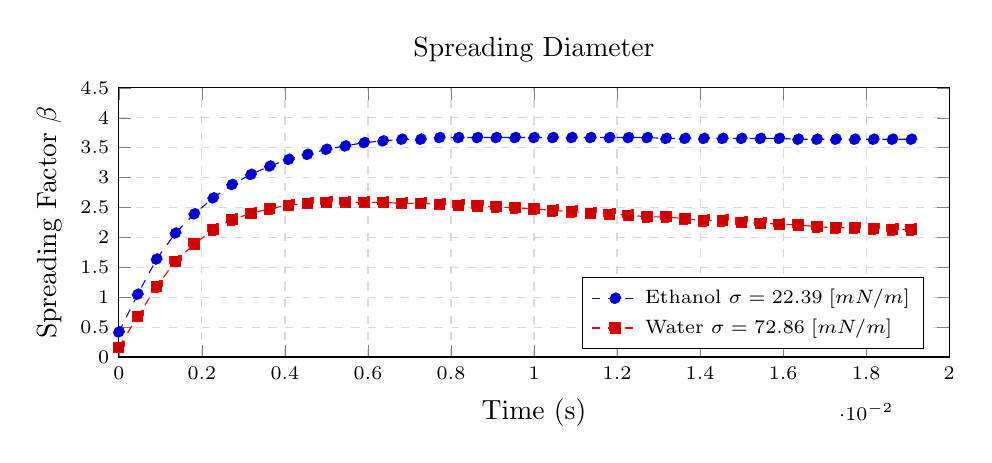
\begin{tikzpicture}
\begin{axis}[
	title = {Spreading Diameter},
    tick label style={font=\scriptsize},
    legend style={font=\scriptsize,/tikz/column 2/.style={column sep=5pt},},
    %legend columns=2,
    legend cell align=left,
	legend pos =south east,
    grid=major, % Display a grid
    grid style={dashed,gray!30}, % Set the style
    xlabel={Time (s)},
    ylabel={Spreading Factor $\beta$}, 
    ymin = 0, ymax = 4.5,
    ytick={0,0.5,...,4.5},
    %yticklabels={300,325,350,375,400,425,450,475,500,525},
    xmin = 0, xmax = 0.02,
    %ytick={0,1600,...,11200},
    %yticklabel style={
    %    /pgf/number format/fixed,
    %    /pgf/number format/precision=5},
	%scaled y ticks=false,
    width=1\textwidth, height=5cm,
    cycle list name= color
    ]
\addplot+[dashed]
coordinates {(	0	,	0.420168067	)
(	0.000454545	,	1.050420168	)
(	0.000909091	,	1.638655462	)
(	0.001363636	,	2.072829132	)
(	0.001818182	,	2.394957983	)
(	0.002272727	,	2.661064426	)
(	0.002727273	,	2.885154062	)
(	0.003181818	,	3.053221289	)
(	0.003636364	,	3.193277311	)
(	0.004090909	,	3.305322129	)
(	0.004545455	,	3.389355742	)
(	0.005	,	3.473389356	)
(	0.005454545	,	3.529411765	)
(	0.005909091	,	3.585434174	)
(	0.006363636	,	3.613445378	)
(	0.006818182	,	3.641456583	)
(	0.007272727	,	3.641456583	)
(	0.007727273	,	3.669467787	)
(	0.008181818	,	3.669467787	)
(	0.008636364	,	3.669467787	)
(	0.009090909	,	3.669467787	)
(	0.009545455	,	3.669467787	)
(	0.01	,	3.669467787	)
(	0.010454545	,	3.669467787	)
(	0.010909091	,	3.669467787	)
(	0.011363636	,	3.669467787	)
(	0.011818182	,	3.669467787	)
(	0.012272727	,	3.669467787	)
(	0.012727273	,	3.669467787	)
(	0.013181818	,	3.655462185	)
(	0.013636364	,	3.655462185	)
(	0.014090909	,	3.655462185	)
(	0.014545455	,	3.655462185	)
(	0.015	,	3.655462185	)
(	0.015454545	,	3.655462185	)
(	0.015909091	,	3.655462185	)
(	0.016363636	,	3.641456583	)
(	0.016818182	,	3.641456583	)
(	0.017272727	,	3.641456583	)
(	0.017727273	,	3.641456583	)
(	0.018181818	,	3.641456583	)
(	0.018636364	,	3.641456583	)
(	0.019090909	,	3.641456583	)
};
\addlegendentry{Ethanol $\sigma=22.39 \; [mN/m]$}

\addplot+[dashed]
coordinates {(	0	,	0.166303558	)
(	0.000454545	,	0.680332739	)
(	0.000909091	,	1.179243415	)
(	0.001363636	,	1.602561563	)
(	0.001818182	,	1.889813164	)
(	0.002272727	,	2.131709249	)
(	0.002727273	,	2.298012808	)
(	0.003181818	,	2.403842345	)
(	0.003636364	,	2.479434872	)
(	0.004090909	,	2.539908893	)
(	0.004545455	,	2.570145903	)
(	0.005	,	2.585264409	)
(	0.005454545	,	2.585264409	)
(	0.005909091	,	2.585264409	)
(	0.006363636	,	2.585264409	)
(	0.006818182	,	2.570145903	)
(	0.007272727	,	2.570145903	)
(	0.007727273	,	2.555027398	)
(	0.008181818	,	2.539908893	)
(	0.008636364	,	2.524790388	)
(	0.009090909	,	2.509671882	)
(	0.009545455	,	2.494553377	)
(	0.01	,	2.479434872	)
(	0.010454545	,	2.449197861	)
(	0.010909091	,	2.434079356	)
(	0.011363636	,	2.403842345	)
(	0.011818182	,	2.38872384	)
(	0.012272727	,	2.373605334	)
(	0.012727273	,	2.343368324	)
(	0.013181818	,	2.343368324	)
(	0.013636364	,	2.313131313	)
(	0.014090909	,	2.282894303	)
(	0.014545455	,	2.282894303	)
(	0.015	,	2.252657292	)
(	0.015454545	,	2.237538787	)
(	0.015909091	,	2.222420281	)
(	0.016363636	,	2.207301776	)
(	0.016818182	,	2.177064765	)
(	0.017272727	,	2.16194626	)
(	0.017727273	,	2.16194626	)
(	0.018181818	,	2.146827755	)
(	0.018636364	,	2.131709249	)
(	0.019090909	,	2.131709249	)
};
\addlegendentry{Water $\sigma=72.86 \; [mN/m]$}
\end{axis}
\end{tikzpicture}
\caption{Spreading Factor along time for a water and ethanol droplet with an impact velocity of 0.8 m/s at $\Delta T=20ºC$ from saturation }
\label{fig:ethdiameter}
\end{figure}
\par The spreading factor obtained for water and ethanol droplets is depicted in Figure\ref{fig:ethdiameter}. The maximum spreading factor is reached at 8ms after impact for ethanol and 4 ms after impact for water. Furthermore, ethanol droplet does not recoil but continues the spreading up to very later times after impact in a regime that is governed by capillarity. Naturally the wetted area of the spreading ethanol droplet is larger than that of water. Qualitative high-speed images of both water and ethanol droplets, shown in Figure \ref{fig:ethhs} clearly show the differences quantitatively observed in Figure \ref{fig:ethdiameter}.\\

\begin{figure}[h!]
\centering
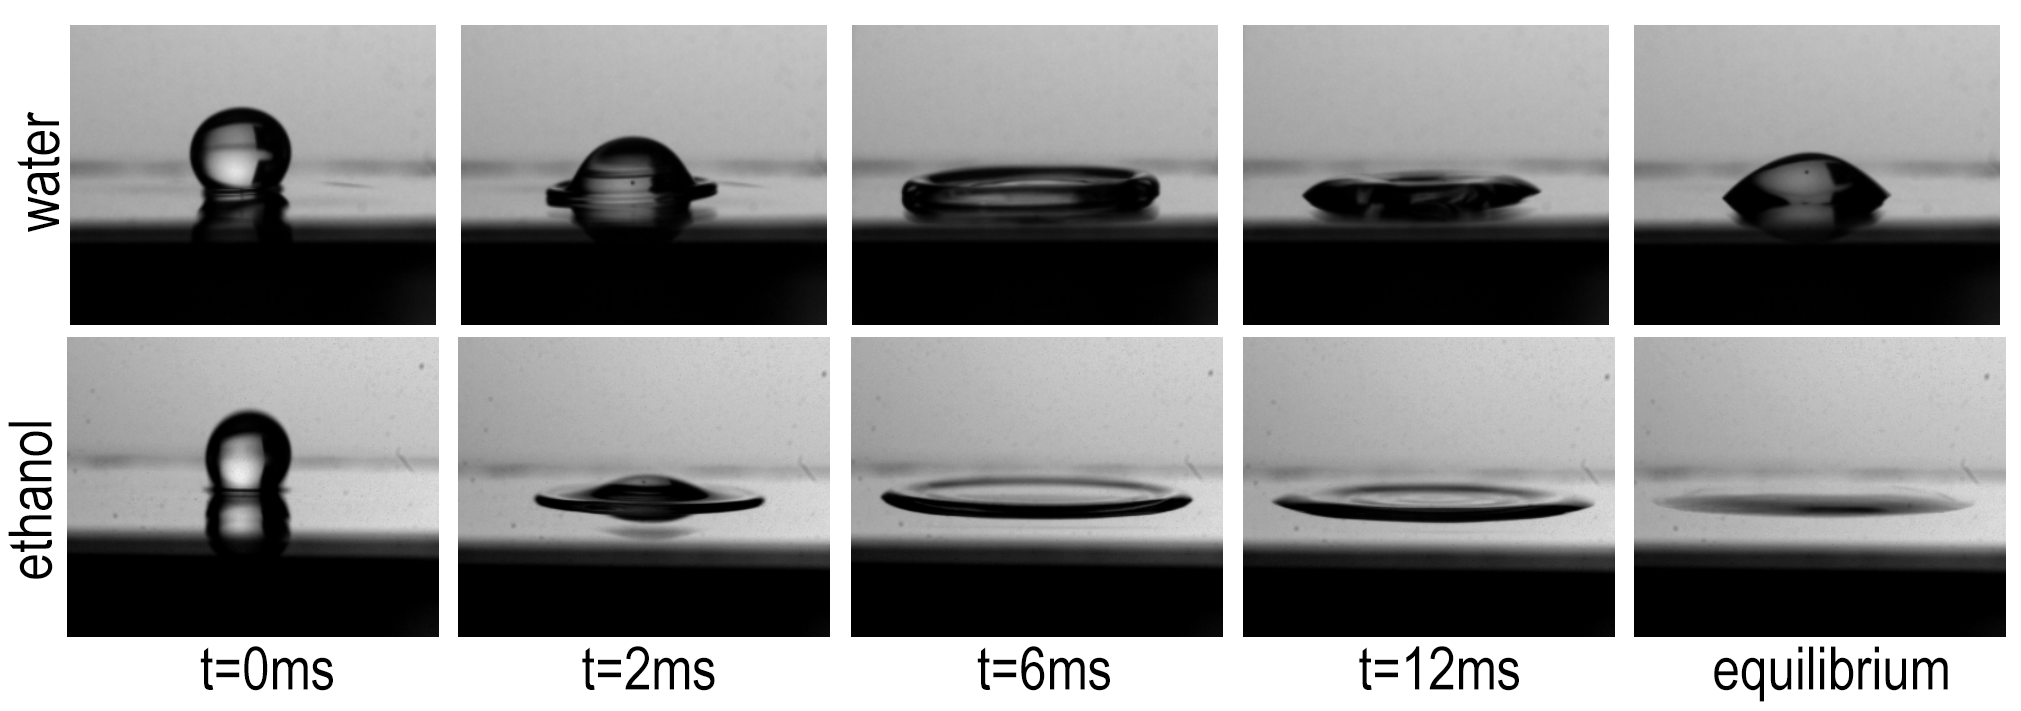
\includegraphics[width=1\linewidth]{Figures/5.Chapter/hsetanol.png}
\caption{High speed images for a water and ethanol droplet impact at the velocity of 0.8 m/s}
\label{fig:ethhs}
\end{figure}

\par To compare the two liquids under similar conditions of initial foil temperature, the first approach was to consider the same temperature difference from the saturation temperature of each liquid. So initial foil temperatures were addressed to compare the two liquids for $\Delta T=20ºC$ and $\Delta T=40ºC$. However, the obtained results showed that this was not a good approach since the temperature influence is relative to the initial foil temperature (i.e. the relative percentage of temperature decay from the saturation temperature) so a new non dimensional temperature is used instead, as depicted in Figure \ref{fig:ethtemp}.\\
\par The results shown in this Figure are in agreement with those reported in Figure \ref{fig:ethdiameter} in the sense that they confirm the larger spreading diameter and the delay in the spreading of the ethanol droplet. The lamella rim, previously identified for water liquids, is also less visible in the ethanol spreading. This is mainly due to the lower thickness of the lamella of the ethanol droplet. The fact that water reaches lower temperatures is mostly related to the worse thermal properties of the ethanol.\\

\begin{figure}[h]
\centering
\subfigure[2 ms]{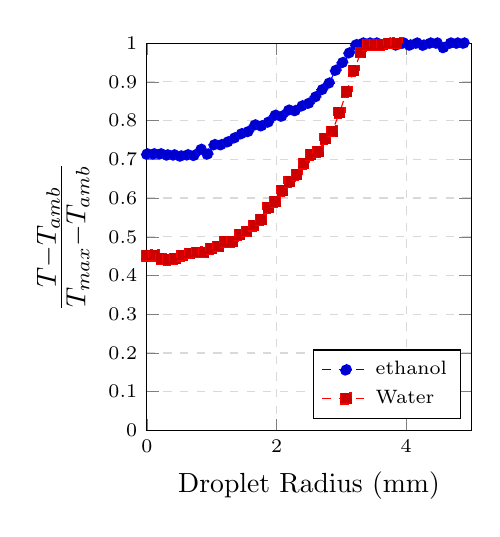
\begin{tikzpicture}
\begin{axis}[
	%title = {13ms},
    tick label style={font=\scriptsize},
    legend style={font=\scriptsize,/tikz/column 2/.style={column sep=5pt},},
    %legend columns=2,
    legend cell align=left,
	legend pos =south east,
    grid=major, % Display a grid
    grid style={dashed,gray!30}, % Set the style
    xlabel={Droplet Radius (mm)},
    ylabel={\Large{$\frac{T-T_{amb}}{T_{max}-T_{amb}}$}}, 
    ymin = 0, ymax = 1,
    ytick={0,0.1,...,1},
    %yticklabels={300,325,350,375,400,425,450,475,500,525},
    xmin = 0, xmax = 5,
    %ytick={0,1600,...,11200},
    %yticklabel style={
    %    /pgf/number format/fixed,
    %    /pgf/number format/precision=5},
	%scaled y ticks=false,
    width=0.47\textwidth, 
    height=6.5cm,
    cycle list name= color
    ]
\addplot+[dashed]
coordinates {(	0	,	0.713749465	)
(	0.104	,	0.714019761	)
(	0.208	,	0.714019761	)
(	0.312	,	0.71120584	)
(	0.416	,	0.71120584	)
(	0.52	,	0.708509477	)
(	0.624	,	0.71152371	)
(	0.728	,	0.710183673	)
(	0.832	,	0.725523462	)
(	0.936	,	0.71347848	)
(	1.04	,	0.737771091	)
(	1.144	,	0.737705876	)
(	1.248	,	0.745195398	)
(	1.352	,	0.755460834	)
(	1.456	,	0.765999807	)
(	1.56	,	0.771671404	)
(	1.664	,	0.788605665	)
(	1.768	,	0.786621648	)
(	1.872	,	0.796190946	)
(	1.976	,	0.813548265	)
(	2.08	,	0.811439765	)
(	2.184	,	0.826796627	)
(	2.288	,	0.825809356	)
(	2.392	,	0.837927288	)
(	2.496	,	0.844826606	)
(	2.6	,	0.861372049	)
(	2.704	,	0.88008609	)
(	2.808	,	0.896768324	)
(	2.912	,	0.929980829	)
(	3.016	,	0.949849396	)
(	3.12	,	0.974891492	)
(	3.224	,	0.99575182	)
(	3.328	,	1	)
(	3.432	,	1	)
(	3.536	,	1	)
(	3.64	,	0.995483735	)
(	3.744	,	1	)
(	3.848	,	0.995245434	)
(	3.952	,	1	)
(	4.056	,	0.994982499	)
(	4.16	,	1	)
(	4.264	,	0.994691043	)
(	4.368	,	1	)
(	4.472	,	1	)
(	4.576	,	0.988621691	)
(	4.68	,	1	)
(	4.784	,	1	)
(	4.888	,	1	)
};
\addlegendentry{ethanol}

\addplot+[dashed]
coordinates {(	0	,	0.451862258	)
(	0.11	,	0.451862258	)
(	0.22	,	0.443203195	)
(	0.33	,	0.440238544	)
(	0.44	,	0.44313005	)
(	0.55	,	0.451877785	)
(	0.66	,	0.45767581	)
(	0.77	,	0.460586008	)
(	0.88	,	0.460586008	)
(	0.99	,	0.469373642	)
(	1.1	,	0.475280359	)
(	1.21	,	0.487212523	)
(	1.32	,	0.487212523	)
(	1.43	,	0.50541746	)
(	1.54	,	0.514662986	)
(	1.65	,	0.529219753	)
(	1.76	,	0.543603017	)
(	1.87	,	0.575024805	)
(	1.98	,	0.589936631	)
(	2.09	,	0.618739307	)
(	2.2	,	0.642225952	)
(	2.31	,	0.660638103	)
(	2.42	,	0.689371721	)
(	2.53	,	0.711522782	)
(	2.64	,	0.719978372	)
(	2.75	,	0.753210196	)
(	2.86	,	0.772698115	)
(	2.97	,	0.820128713	)
(	3.08	,	0.873929253	)
(	3.19	,	0.928211073	)
(	3.3	,	0.976087543	)
(	3.41	,	0.995964175	)
(	3.52	,	0.995901193	)
(	3.63	,	0.995744732	)
(	3.74	,	1	)
(	3.85	,	1	)
};
\addlegendentry{Water}

\end{axis}
\end{tikzpicture}}
\subfigure[6 ms]{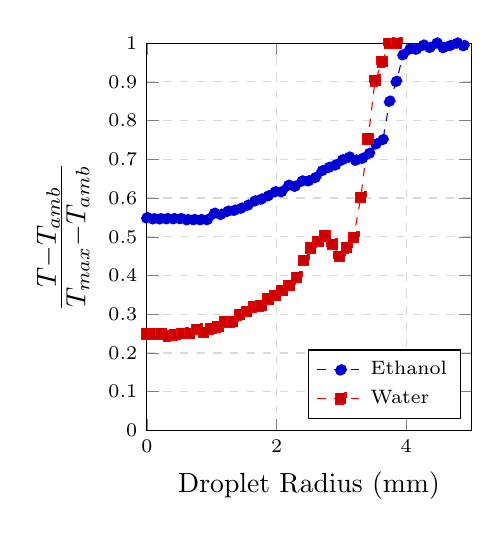
\begin{tikzpicture}
\begin{axis}[
	%title = {0.8 m/s || 13ms},
    tick label style={font=\scriptsize},
    legend style={font=\scriptsize,/tikz/column 2/.style={column sep=5pt},},
    %legend columns=2,
    legend cell align=left,
	legend pos =south east,
    grid=major, % Display a grid
    grid style={dashed,gray!30}, % Set the style
    xlabel={Droplet Radius (mm)},
    ylabel={\Large{$\frac{T-T_{amb}}{T_{max}-T_{amb}}$}}, 
    ymin = 0, ymax = 1,
    ytick={0,0.1,...,1},
    %yticklabels={300,325,350,375,400,425,450,475,500,525},
    xmin = 0, xmax = 5,
    %ytick={0,1600,...,11200},
    %yticklabel style={
    %    /pgf/number format/fixed,
    %    /pgf/number format/precision=5},
	%scaled y ticks=false,
    width=0.47\textwidth, 
    height=6.5cm,
    cycle list name= color
    ]
\addplot+[dashed]
coordinates {(	0	,	0.549083129	)
(	0.104	,	0.546405797	)
(	0.208	,	0.546405797	)
(	0.312	,	0.546679498	)
(	0.416	,	0.546679498	)
(	0.52	,	0.546963482	)
(	0.624	,	0.544146891	)
(	0.728	,	0.544317442	)
(	0.832	,	0.544146891	)
(	0.936	,	0.544489767	)
(	1.04	,	0.560522446	)
(	1.144	,	0.557908066	)
(	1.248	,	0.565838227	)
(	1.352	,	0.568450792	)
(	1.456	,	0.573783086	)
(	1.56	,	0.581565998	)
(	1.664	,	0.592477222	)
(	1.768	,	0.597380792	)
(	1.872	,	0.605722005	)
(	1.976	,	0.616085999	)
(	2.08	,	0.616604013	)
(	2.184	,	0.632781734	)
(	2.288	,	0.630523084	)
(	2.392	,	0.643877098	)
(	2.496	,	0.644687777	)
(	2.6	,	0.652944904	)
(	2.704	,	0.670614691	)
(	2.808	,	0.679027954	)
(	2.912	,	0.685488529	)
(	3.016	,	0.698726167	)
(	3.12	,	0.705508954	)
(	3.224	,	0.697709267	)
(	3.328	,	0.702753051	)
(	3.432	,	0.715493219	)
(	3.536	,	0.739677632	)
(	3.64	,	0.750816301	)
(	3.744	,	0.849862624	)
(	3.848	,	0.901300664	)
(	3.952	,	0.970011476	)
(	4.056	,	0.984888014	)
(	4.16	,	0.984459331	)
(	4.264	,	0.994691043	)
(	4.368	,	0.989043361	)
(	4.472	,	1	)
(	4.576	,	0.988621691	)
(	4.68	,	0.993904718	)
(	4.784	,	1	)
(	4.888	,	0.993537586	)
};
\addlegendentry{Ethanol}

\addplot+[dashed]
coordinates {(	0	,	0.248982722	)
(	0.11	,	0.248982722	)
(	0.22	,	0.249805892	)
(	0.33	,	0.244795846	)
(	0.44	,	0.247700134	)
(	0.55	,	0.250613773	)
(	0.66	,	0.250613773	)
(	0.77	,	0.261441892	)
(	0.88	,	0.253536836	)
(	0.99	,	0.262363317	)
(	1.1	,	0.268296145	)
(	1.21	,	0.280281057	)
(	1.32	,	0.280281057	)
(	1.43	,	0.298566471	)
(	1.54	,	0.307852868	)
(	1.65	,	0.318875282	)
(	1.76	,	0.322003741	)
(	1.87	,	0.339263602	)
(	1.98	,	0.348820007	)
(	2.09	,	0.361727603	)
(	2.2	,	0.374830928	)
(	2.31	,	0.395848829	)
(	2.42	,	0.439310776	)
(	2.53	,	0.470980955	)
(	2.64	,	0.488614372	)
(	2.75	,	0.502867701	)
(	2.86	,	0.481046752	)
(	2.97	,	0.449608484	)
(	3.08	,	0.471965743	)
(	3.19	,	0.499090216	)
(	3.3	,	0.602531448	)
(	3.41	,	0.752933261	)
(	3.52	,	0.90373183	)
(	3.63	,	0.951500779	)
(	3.74	,	1	)
(	3.85	,	0.999895493	)
};
\addlegendentry{Water}

\end{axis}
\end{tikzpicture}}
\subfigure[12 ms]{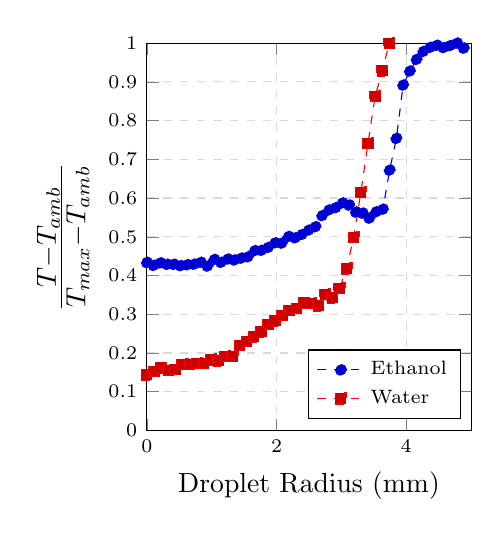
\begin{tikzpicture}
\begin{axis}[
	%title = {0.8 m/s || 13ms},
    tick label style={font=\scriptsize},
    legend style={font=\scriptsize,/tikz/column 2/.style={column sep=5pt},},
    %legend columns=2,
    legend cell align=left,
	legend pos =south east,
    grid=major, % Display a grid
    grid style={dashed,gray!30}, % Set the style
    xlabel={Droplet Radius (mm)},
    ylabel={\Large{$\frac{T-T_{amb}}{T_{max}-T_{amb}}$}}, 
    ymin = 0, ymax = 1,
    ytick={0,0.1,...,1},
    %yticklabels={300,325,350,375,400,425,450,475,500,525},
    xmin = 0, xmax = 5,
    %ytick={0,1600,...,11200},
    %yticklabel style={
    %    /pgf/number format/fixed,
    %    /pgf/number format/precision=5},
	%scaled y ticks=false,
    width=0.47\textwidth, 
    height=6.5cm,
    cycle list name= color
    ]
\addplot+[dashed]
coordinates {(	0	,	0.433801984	)
(	0.104	,	0.42621613	)
(	0.208	,	0.432574638	)
(	0.312	,	0.428932721	)
(	0.416	,	0.428932721	)
(	0.52	,	0.425435898	)
(	0.624	,	0.427839123	)
(	0.728	,	0.429168872	)
(	0.832	,	0.433984115	)
(	0.936	,	0.424423495	)
(	1.04	,	0.441294219	)
(	1.144	,	0.434124853	)
(	1.248	,	0.442479601	)
(	1.352	,	0.440094496	)
(	1.456	,	0.444882035	)
(	1.56	,	0.448426112	)
(	1.664	,	0.464155088	)
(	1.768	,	0.465111906	)
(	1.872	,	0.472594756	)
(	1.976	,	0.484370934	)
(	2.08	,	0.483607472	)
(	2.184	,	0.500603592	)
(	2.288	,	0.497349794	)
(	2.392	,	0.505919951	)
(	2.496	,	0.517226058	)
(	2.6	,	0.525857811	)
(	2.704	,	0.554732782	)
(	2.808	,	0.56925987	)
(	2.912	,	0.575201664	)
(	3.016	,	0.587376323	)
(	3.12	,	0.58177078	)
(	3.224	,	0.563952432	)
(	3.328	,	0.560973814	)
(	3.432	,	0.548240482	)
(	3.536	,	0.564601593	)
(	3.64	,	0.571117172	)
(	3.744	,	0.672213348	)
(	3.848	,	0.754030516	)
(	3.952	,	0.891761443	)
(	4.056	,	0.927886511	)
(	4.16	,	0.958132148	)
(	4.264	,	0.978632265	)
(	4.368	,	0.989043361	)
(	4.472	,	0.994366339	)
(	4.576	,	0.988621691	)
(	4.68	,	0.993904718	)
(	4.784	,	1	)
(	4.888	,	0.987044307	)
};
\addlegendentry{Ethanol}

\addplot+[dashed]
coordinates {(	0	,	0.143423031	)
(	0.11	,	0.152940399	)
(	0.22	,	0.161852829	)
(	0.33	,	0.155325188	)
(	0.44	,	0.158324498	)
(	0.55	,	0.170850832	)
(	0.66	,	0.170850832	)
(	0.77	,	0.173869531	)
(	0.88	,	0.173869531	)
(	0.99	,	0.182984794	)
(	1.1	,	0.179594362	)
(	1.21	,	0.191971391	)
(	1.32	,	0.191971391	)
(	1.43	,	0.22037243	)
(	1.54	,	0.229962656	)
(	1.65	,	0.24255453	)
(	1.76	,	0.255018102	)
(	1.87	,	0.273878127	)
(	1.98	,	0.283747196	)
(	2.09	,	0.297077098	)
(	2.2	,	0.310609133	)
(	2.31	,	0.315253033	)
(	2.42	,	0.329212343	)
(	2.53	,	0.328375143	)
(	2.64	,	0.322455312	)
(	2.75	,	0.351787779	)
(	2.86	,	0.342120193	)
(	2.97	,	0.366838812	)
(	3.08	,	0.418050199	)
(	3.19	,	0.499193253	)
(	3.3	,	0.615130812	)
(	3.41	,	0.741623756	)
(	3.52	,	0.862494546	)
(	3.63	,	0.928955596	)
(	3.74	,	1	)
(	3.85	,	1.01842101	)
};
\addlegendentry{Water}

\end{axis}
\end{tikzpicture}}
\subfigure[24 ms]{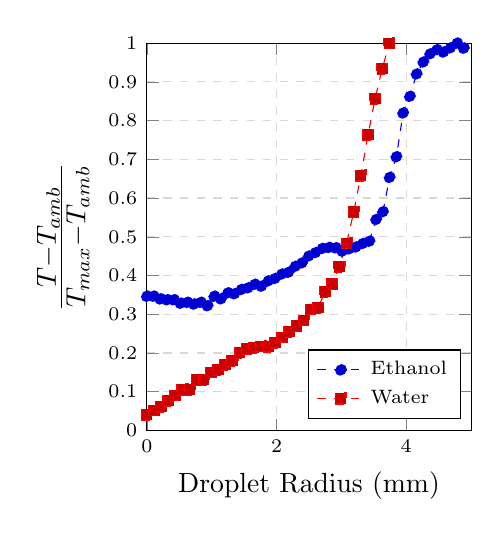
\begin{tikzpicture}
\begin{axis}[
	%title = {0.8 m/s || 13ms},
    tick label style={font=\scriptsize},
    legend style={font=\scriptsize,/tikz/column 2/.style={column sep=5pt},},
    %legend columns=2,
    legend cell align=left,
	legend pos =south east,
    grid=major, % Display a grid
    grid style={dashed,gray!30}, % Set the style
    xlabel={Droplet Radius (mm)},
    ylabel={\Large{$\frac{T-T_{amb}}{T_{max}-T_{amb}}$}}, 
    ymin = 0, ymax = 1,
    ytick={0,0.1,...,1},
    %yticklabels={300,325,350,375,400,425,450,475,500,525},
    xmin = 0, xmax = 5,
    %ytick={0,1600,...,11200},
    %yticklabel style={
    %    /pgf/number format/fixed,
    %    /pgf/number format/precision=5},
	%scaled y ticks=false,
    width=0.47\textwidth, 
    height=6.5cm,
    cycle list name= color
    ]
\addplot+[dashed]
coordinates {(	0	,	0.346625417	)
(	0.104	,	0.346566747	)
(	0.208	,	0.339629094	)
(	0.312	,	0.337422351	)
(	0.416	,	0.337422351	)
(	0.52	,	0.328547695	)
(	0.624	,	0.330741789	)
(	0.728	,	0.326369652	)
(	0.832	,	0.330741789	)
(	0.936	,	0.322060952	)
(	1.04	,	0.346491418	)
(	1.144	,	0.339923936	)
(	1.248	,	0.355225997	)
(	1.352	,	0.353024989	)
(	1.456	,	0.363954729	)
(	1.56	,	0.368178469	)
(	1.664	,	0.377255675	)
(	1.768	,	0.372683905	)
(	1.872	,	0.386047927	)
(	1.976	,	0.392486416	)
(	2.08	,	0.403641967	)
(	2.184	,	0.408472654	)
(	2.288	,	0.423725992	)
(	2.392	,	0.432574638	)
(	2.496	,	0.450295908	)
(	2.6	,	0.459170303	)
(	2.704	,	0.469798481	)
(	2.808	,	0.472508181	)
(	2.912	,	0.471606677	)
(	3.016	,	0.46319735	)
(	3.12	,	0.468828074	)
(	3.224	,	0.473664234	)
(	3.328	,	0.482532407	)
(	3.432	,	0.488572733	)
(	3.536	,	0.54481948	)
(	3.64	,	0.564601593	)
(	3.744	,	0.653495151	)
(	3.848	,	0.706651618	)
(	3.952	,	0.819703615	)
(	4.056	,	0.862598574	)
(	4.16	,	0.920334615	)
(	4.264	,	0.951414808	)
(	4.368	,	0.972433581	)
(	4.472	,	0.983026006	)
(	4.576	,	0.97714404	)
(	4.68	,	0.987781579	)
(	4.784	,	1	)
(	4.888	,	0.987044307	)
};
\addlegendentry{Ethanol}

\addplot+[dashed]
coordinates {(	0	,	0.040715756	)
(	0.11	,	0.052564398	)
(	0.22	,	0.061888861	)
(	0.33	,	0.076638338	)
(	0.44	,	0.091180728	)
(	0.55	,	0.105525431	)
(	0.66	,	0.105525431	)
(	0.77	,	0.130487824	)
(	0.88	,	0.130487824	)
(	0.99	,	0.150647768	)
(	1.1	,	0.157057961	)
(	1.21	,	0.170007197	)
(	1.32	,	0.180454298	)
(	1.43	,	0.200210986	)
(	1.54	,	0.210244581	)
(	1.65	,	0.213612765	)
(	1.76	,	0.216992945	)
(	1.87	,	0.216759401	)
(	1.98	,	0.22708473	)
(	2.09	,	0.24103089	)
(	2.2	,	0.255188529	)
(	2.31	,	0.269565516	)
(	2.42	,	0.284170184	)
(	2.53	,	0.313206809	)
(	2.64	,	0.316970665	)
(	2.75	,	0.357936866	)
(	2.86	,	0.378008767	)
(	2.97	,	0.42273945	)
(	3.08	,	0.483648605	)
(	3.19	,	0.563946389	)
(	3.3	,	0.658378026	)
(	3.41	,	0.76294436	)
(	3.52	,	0.856699265	)
(	3.63	,	0.934006873	)
(	3.74	,	1	)
(	3.85	,	1.034978696	)
};
\addlegendentry{Water}

\end{axis}
\end{tikzpicture}}
\caption{Average temperature along the radius for Ethanol and Water for a droplet impacting at 0.8m/s on a foil initially with $\Delta T=20ºC$ under saturation}
\label{fig:ethtemp}
\end{figure}

\par The heat flux can also be compared between both liquids. Looking at the plots in Figure \ref{fig:ethflux}, an elevated heat flux difference is visible between water and ethanol. The water droplet extracts more heat from the foil than the ethanol droplet.This trend is however affected by the slightly smaller initial diameter of the ethanol droplet (d0=2mm for ethanol and 3mm for water) and due to the aforementioned different temperature difference between the initial foil temperature and the saturation temperature which is actually much different (in percentage).\\

\begin{figure}[h]
\centering
\subfigure[2 ms]{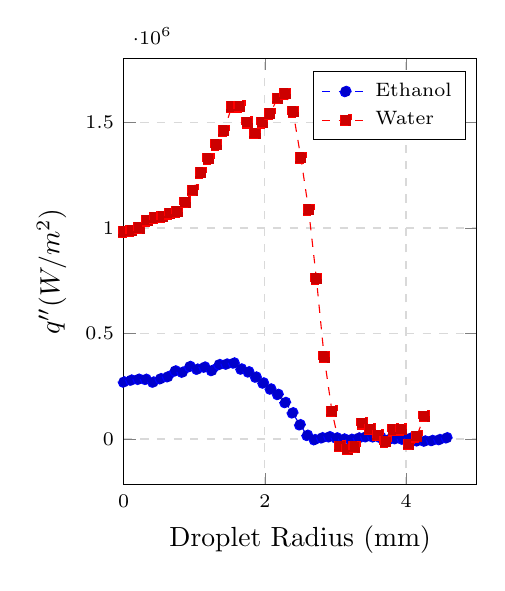
\begin{tikzpicture}
\begin{axis}[
	%title = {107 ºC || $T_{amb}=24$},
    tick label style={font=\scriptsize},
    legend style={font=\scriptsize,/tikz/column 2/.style={column sep=5pt},},
    %legend columns=2,
    legend cell align=left,
	legend pos =north east,
    grid=major, % Display a grid
    grid style={dashed,gray!30}, % Set the style
    xlabel={Droplet Radius (mm)},
    ylabel={$q''(W/m^2)$}, 
    %ymin = 55, ymax = 113,
    %ytick={60,70,...,100,110},
    %yticklabels={300,325,350,375,400,425,450,475,500,525},
    xmin = 0, xmax = 5,
    %ytick={0,1600,...,11200},
    %yticklabel style={
    %    /pgf/number format/fixed,
    %    /pgf/number format/precision=5},
	%scaled y ticks=false,
    width=0.5\textwidth, height=7cm,
    cycle list name= color
    ]
\addplot+[dashed]
coordinates {(	0	,	270120.8105	)
(	0.104	,	278913.13	)
(	0.208	,	283066.4518	)
(	0.312	,	282646.2162	)
(	0.416	,	269592.9712	)
(	0.52	,	285594.4895	)
(	0.624	,	295090.8064	)
(	0.728	,	322357.8767	)
(	0.832	,	316714.479	)
(	0.936	,	343445.3341	)
(	1.04	,	330718.507	)
(	1.144	,	340568.6424	)
(	1.248	,	324544.2497	)
(	1.352	,	352352.1723	)
(	1.456	,	354930.4151	)
(	1.56	,	359917.3186	)
(	1.664	,	331443.584	)
(	1.768	,	318066.746	)
(	1.872	,	293193.3436	)
(	1.976	,	265166.8856	)
(	2.08	,	236913.8287	)
(	2.184	,	211064.9953	)
(	2.288	,	172895.2388	)
(	2.392	,	123968.5451	)
(	2.496	,	67484.42808	)
(	2.6	,	17485.77352	)
(	2.704	,	-3159.175389	)
(	2.808	,	5634.47142	)
(	2.912	,	10660.58323	)
(	3.016	,	5001.018204	)
(	3.12	,	-317.8234826	)
(	3.224	,	-1751.982475	)
(	3.328	,	4538.448393	)
(	3.432	,	10831.93505	)
(	3.536	,	10414.90159	)
(	3.64	,	7576.893178	)
(	3.744	,	-4184.03352	)
(	3.848	,	1743.522936	)
(	3.952	,	-592.3329438	)
(	4.056	,	3303.30417	)
(	4.16	,	-8583.954418	)
(	4.264	,	-9762.561903	)
(	4.368	,	-7116.774112	)
(	4.472	,	-2756.514952	)
(	4.576	,	5634.282847	)
};
\addlegendentry{Ethanol}

\addplot+[dashed]
coordinates {(	0	,	982089.2242	)
(	0.11	,	986559.7305	)
(	0.22	,	999747.4309	)
(	0.33	,	1035364.347	)
(	0.44	,	1049283.945	)
(	0.55	,	1053120.393	)
(	0.65	,	1068631.742	)
(	0.76	,	1076954.643	)
(	0.87	,	1121386.9	)
(	0.98	,	1178256.05	)
(	1.09	,	1261378.47	)
(	1.2	,	1327056.42	)
(	1.31	,	1393696.902	)
(	1.42	,	1460274.884	)
(	1.53	,	1574936.222	)
(	1.64	,	1575660.786	)
(	1.75	,	1499525.579	)
(	1.86	,	1449022.358	)
(	1.96	,	1499662.339	)
(	2.07	,	1540313.795	)
(	2.18	,	1614313.74	)
(	2.29	,	1635300.374	)
(	2.4	,	1549877.215	)
(	2.51	,	1331868.982	)
(	2.62	,	1085363.344	)
(	2.73	,	759206.8787	)
(	2.84	,	388588.3723	)
(	2.95	,	131341.4508	)
(	3.06	,	-34143.38797	)
(	3.17	,	-49030.87567	)
(	3.27	,	-37679.13294	)
(	3.38	,	73913.01076	)
(	3.49	,	47158.40863	)
(	3.6	,	18684.75783	)
(	3.71	,	-12798.88057	)
(	3.82	,	44948.25807	)
(	3.93	,	45229.68041	)
(	4.04	,	-25391.89314	)
(	4.15	,	12194.80767	)
(	4.26	,	107861.5786	)
};
\addlegendentry{Water}
\end{axis}
\end{tikzpicture}}
\subfigure[4 ms]{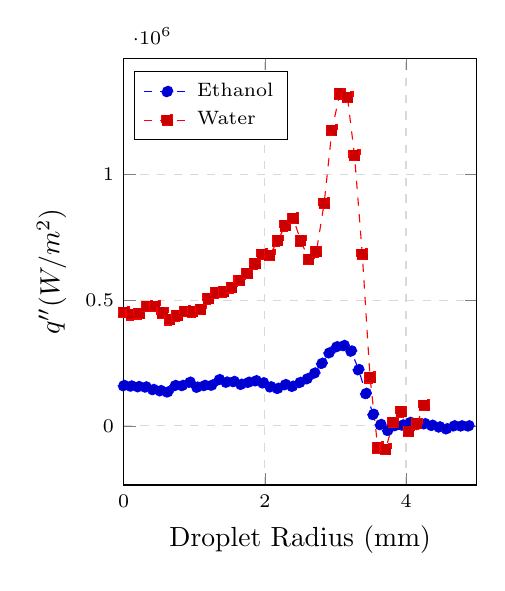
\begin{tikzpicture}
\begin{axis}[
	%title = {107 ºC || $T_{amb}=24$},
    tick label style={font=\scriptsize},
    legend style={font=\scriptsize,/tikz/column 2/.style={column sep=5pt},},
    %legend columns=2,
    legend cell align=left,
	legend pos =north west,
    grid=major, % Display a grid
    grid style={dashed,gray!30}, % Set the style
    xlabel={Droplet Radius (mm)},
    ylabel={$q''(W/m^2)$}, 
    %ymin = 55, ymax = 113,
    %ytick={60,70,...,100,110},
    %yticklabels={300,325,350,375,400,425,450,475,500,525},
    xmin = 0, xmax = 5,
    %ytick={0,1600,...,11200},
    %yticklabel style={
    %    /pgf/number format/fixed,
    %    /pgf/number format/precision=5},
	%scaled y ticks=false,
    width=0.5\textwidth, height=7cm,
    cycle list name= color
    ]
\addplot+[dashed]
coordinates {(	0	,	160521.1529	)
(	0.104	,	158654.7709	)
(	0.208	,	156294.3565	)
(	0.312	,	154809.2823	)
(	0.416	,	144775.6004	)
(	0.52	,	140089.5364	)
(	0.624	,	135245.3481	)
(	0.728	,	160461.9758	)
(	0.832	,	160864.2492	)
(	0.936	,	173671.006	)
(	1.04	,	153998.2471	)
(	1.144	,	160805.7289	)
(	1.248	,	162182.2259	)
(	1.352	,	183961.9004	)
(	1.456	,	174097.6949	)
(	1.56	,	176472.8989	)
(	1.664	,	165544.6491	)
(	1.768	,	173592.9555	)
(	1.872	,	179571.4659	)
(	1.976	,	171265.3226	)
(	2.08	,	155368.661	)
(	2.184	,	149379.2787	)
(	2.288	,	164131.8629	)
(	2.392	,	157670.4869	)
(	2.496	,	172711.5733	)
(	2.6	,	187707.2273	)
(	2.704	,	210188.7377	)
(	2.808	,	248914.6145	)
(	2.912	,	290899.2612	)
(	3.016	,	314840.2327	)
(	3.12	,	319779.2497	)
(	3.224	,	297822.0353	)
(	3.328	,	223820.369	)
(	3.432	,	129122.6812	)
(	3.536	,	45761.4763	)
(	3.64	,	5338.465878	)
(	3.744	,	-17682.1412	)
(	3.848	,	1269.769144	)
(	3.952	,	3513.351142	)
(	4.056	,	13549.27605	)
(	4.16	,	5696.230189	)
(	4.264	,	8522.392842	)
(	4.368	,	2169.931835	)
(	4.472	,	-4208.231498	)
(	4.576	,	-11448.69048	)
(	4.68	,	1	)
(	4.784	,	1	)
(	4.888	,	1	)
};
\addlegendentry{Ethanol}

\addplot+[dashed]
coordinates {(	0	,	452958.8884	)
(	0.11	,	443672.2939	)
(	0.22	,	447691.5594	)
(	0.33	,	476523.1849	)
(	0.44	,	476471.8183	)
(	0.55	,	450806.3468	)
(	0.65	,	423782.5444	)
(	0.76	,	438179.2292	)
(	0.87	,	456897.6624	)
(	0.98	,	454134.3395	)
(	1.09	,	464286.0605	)
(	1.2	,	506555.4293	)
(	1.31	,	529832.2559	)
(	1.42	,	533809	)
(	1.53	,	551142.8174	)
(	1.64	,	579323.7681	)
(	1.75	,	608315.9539	)
(	1.86	,	645875.8736	)
(	1.96	,	683086.4821	)
(	2.07	,	680217.8765	)
(	2.18	,	737096.0515	)
(	2.29	,	797628.0866	)
(	2.4	,	826481.1812	)
(	2.51	,	736599.5618	)
(	2.62	,	663007.6906	)
(	2.73	,	693457.4194	)
(	2.84	,	886760.2203	)
(	2.95	,	1177186.265	)
(	3.06	,	1321888.579	)
(	3.17	,	1307905.114	)
(	3.27	,	1077377.636	)
(	3.38	,	683874.6368	)
(	3.49	,	192779.5452	)
(	3.6	,	-86073.52402	)
(	3.71	,	-93468.67899	)
(	3.82	,	15343.63931	)
(	3.93	,	56675.86267	)
(	4.04	,	-20794.54961	)
(	4.15	,	8059.529388	)
(	4.26	,	82566.79303	)
};
\addlegendentry{Water}

\end{axis}
\end{tikzpicture}}
\caption{Heat Flux along the radius for Ethanol and Water for a droplet impacting at 0.8m/s on a foil initially with $\Delta T=20ºC$ under saturation}
\label{fig:ethflux}
\end{figure}

\par Hence heat flux isn't directly comparable between experiments, but one may compare the the cooling effectiveness of both liquids as this parameter takes into account both the droplet's initial diameter and thermal properties. The obtained results are depicted in Figure \ref{fig:ethcool}. The results for the ethanol experiment show a better cooling effectiveness. This may seem odd looking at the flux values, which are is much lower for ethanol. However, considering the definition of the cooling effectiveness, the total heat removed is divided by the maximum possible heat removed. Since ethanol has worse thermal properties, the maximum possible heat removed is also lower that of water, so at the end the cooling effectiveness considering the improved wetted area is actually higher for ethanol. One can't conclude that ethanol is a better alternative to water when considering droplet cooling applications. The opposite is true and deductible from observing the heat flux and temperature variation plots. Instead what can be said regarding cooling effectiveness is that low surface tensions are related with higher effectiveness. This can be related to larger spreading and wetted area for the same impact velocity, as aforementioned.

\begin{figure}[h]
\centering
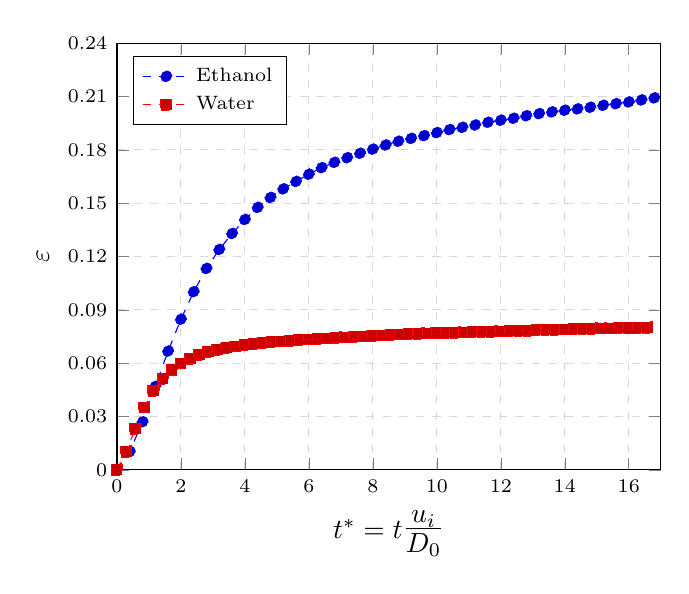
\begin{tikzpicture}
\begin{axis}[
	%title = {$20 ºC || $T_{amb}=24$},
    tick label style={font=\scriptsize},
    legend style={font=\scriptsize,/tikz/column 2/.style={column sep=5pt},},
    %legend columns=2,
    legend cell align=left,
	legend pos =north west,
    grid=major, % Display a grid
    grid style={dashed,gray!30}, % Set the style
    xlabel={$t^*=t$\Large{$\frac{u_i}{D_0}$}},
    ylabel={$\varepsilon$}, 
    ymin = 0, ymax = 0.24,
    ytick={0,0.03,0.06,0.09,0.12,0.15,0.18,0.21,0.24},
    yticklabels={0,0.03,0.06,0.09,0.12,0.15,0.18,0.21,0.24},
    xmin = 0, xmax = 17,
    %ytick={0,1600,...,11200},
    %yticklabel style={
    %    /pgf/number format/fixed,
    %    /pgf/number format/precision=5},
	%scaled y ticks=false,
    width=0.7\textwidth, 
    height=7cm,
    cycle list name= color
    ]
\addplot+[dashed]
coordinates {(	0	,	0	)
(	0.4	,	0.010217771	)
(	0.8	,	0.026957313	)
(	1.2	,	0.046942191	)
(	1.6	,	0.06679577	)
(	2	,	0.084693861	)
(	2.4	,	0.100193383	)
(	2.8	,	0.113269339	)
(	3.2	,	0.123948653	)
(	3.6	,	0.13293841	)
(	4	,	0.14081246	)
(	4.4	,	0.14760748	)
(	4.8	,	0.153196021	)
(	5.2	,	0.158024113	)
(	5.6	,	0.16221596	)
(	6	,	0.166264442	)
(	6.4	,	0.169953672	)
(	6.8	,	0.172957467	)
(	7.2	,	0.17556641	)
(	7.6	,	0.178046374	)
(	8	,	0.180377269	)
(	8.4	,	0.182703585	)
(	8.8	,	0.184826807	)
(	9.2	,	0.186406718	)
(	9.6	,	0.187961307	)
(	10	,	0.189670288	)
(	10.4	,	0.191371542	)
(	10.8	,	0.192642487	)
(	11.2	,	0.193957477	)
(	11.6	,	0.195480766	)
(	12	,	0.19663772	)
(	12.4	,	0.197735327	)
(	12.8	,	0.199162975	)
(	13.2	,	0.200337481	)
(	13.6	,	0.201325276	)
(	14	,	0.202255004	)
(	14.4	,	0.203021435	)
(	14.8	,	0.203938499	)
(	15.2	,	0.20501696	)
(	15.6	,	0.205950537	)
(	16	,	0.206910824	)
(	16.4	,	0.208050946	)
(	16.8	,	0.209206879	)
};
\addlegendentry{Ethanol}
\addplot+[dashed]
coordinates {(	0	,	0	)
(	0.285714286	,	0.010266233	)
(	0.571428571	,	0.022999357	)
(	0.857142857	,	0.035112403	)
(	1.142857143	,	0.044436998	)
(	1.428571429	,	0.051132579	)
(	1.714285714	,	0.056146158	)
(	2	,	0.059853933	)
(	2.285714286	,	0.062591203	)
(	2.571428571	,	0.064757937	)
(	2.857142857	,	0.0663376	)
(	3.142857143	,	0.067623077	)
(	3.428571429	,	0.068750599	)
(	3.714285714	,	0.069577203	)
(	4	,	0.070293613	)
(	4.285714286	,	0.070969048	)
(	4.571428571	,	0.071539897	)
(	4.857142857	,	0.071988407	)
(	5.142857143	,	0.07236088	)
(	5.428571429	,	0.072756921	)
(	5.714285714	,	0.073145343	)
(	6	,	0.073469193	)
(	6.285714286	,	0.073778428	)
(	6.571428571	,	0.074111323	)
(	6.857142857	,	0.074435161	)
(	7.142857143	,	0.074630534	)
(	7.428571429	,	0.074863176	)
(	7.714285714	,	0.075182577	)
(	8	,	0.075455035	)
(	8.285714286	,	0.075793114	)
(	8.571428571	,	0.076035438	)
(	8.857142857	,	0.076227021	)
(	9.142857143	,	0.076492228	)
(	9.428571429	,	0.076623551	)
(	9.714285714	,	0.076777963	)
(	10	,	0.077003192	)
(	10.28571429	,	0.077129222	)
(	10.57142857	,	0.077249244	)
(	10.85714286	,	0.077397712	)
(	11.14285714	,	0.077544384	)
(	11.42857143	,	0.077619809	)
(	11.71428571	,	0.077753859	)
(	12	,	0.077932196	)
(	12.28571429	,	0.078105326	)
(	12.57142857	,	0.078246693	)
(	12.85714286	,	0.078393586	)
(	13.14285714	,	0.078670213	)
(	13.42857143	,	0.078717216	)
(	13.71428571	,	0.078752432	)
(	14	,	0.079006745	)
(	14.28571429	,	0.079234771	)
(	14.57142857	,	0.079359104	)
(	14.85714286	,	0.07945779	)
(	15.14285714	,	0.079607258	)
(	15.42857143	,	0.079668009	)
(	15.71428571	,	0.079781132	)
(	16	,	0.07992979	)
(	16.28571429	,	0.079956177	)
(	16.57142857	,	0.080031454	)
};
\addlegendentry{Water}
\end{axis}
\end{tikzpicture}
\caption{Cooling Effectiveness comparison between water and ethanol for a droplet impacting at 0.8m/s on a foil initially with $\Delta T=20ºC$ under saturation}
\label{fig:ethcool}
\end{figure}

\subsection{Effect of extreme wetting scenarios: Hydrophilic and Super-Hydrophobic surfaces}

\par Wettability plays a big part in interface phenomena, and its effects on heat transfer can also be studied by IR thermography. With this in mind, several stainless steel foils were cleaned and coated to become super-hydrophobic in order to apply the developed techniques to different wettability surfaces. A comparison between the physical phenomena in the different droplet impact phases is shown in Figure \ref{fig:hsshf}. The main difference between this comparison and the latter two is that instead of having an equilibrium phase, the droplet rebounds off the surface. Initially, the evolution looks similar, but in the timestep of 6ms, while the droplet is already receding in the super-hydrophobic, in the hydrophilic surface, it's reaching its maximum diameter. In terms of droplet impact related phenomena, we can see that the lamella also forms a rim near the contact edge, but quickly disappears.

\begin{figure}[h]
\centering
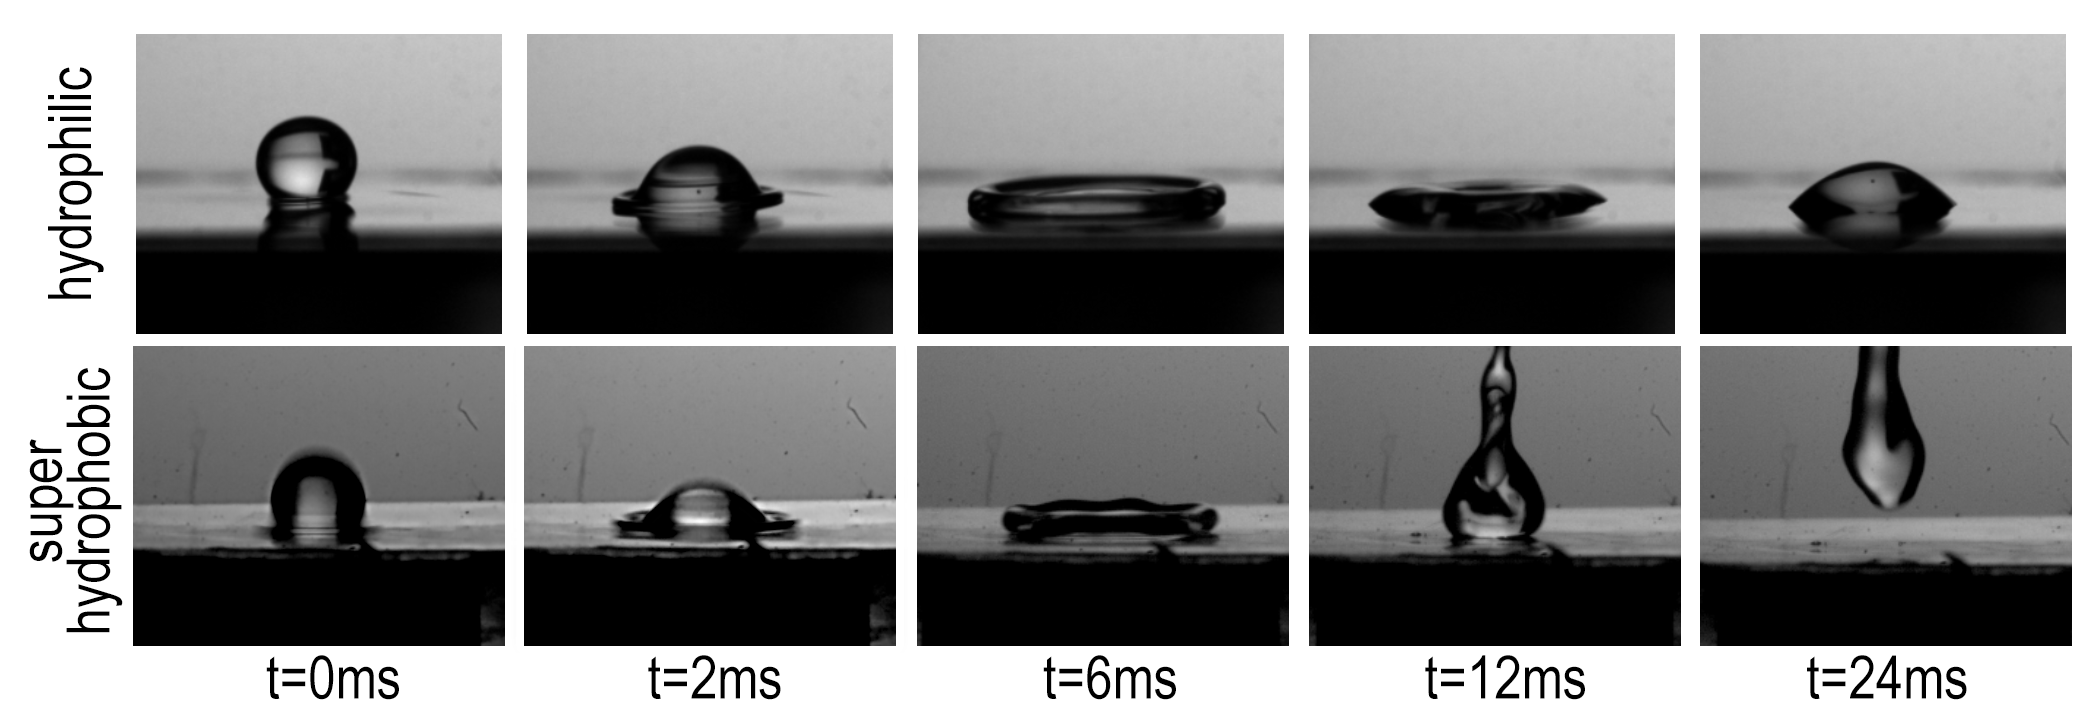
\includegraphics[width=1\linewidth]{Figures/5.Chapter/hsshf.png}
\caption{HS Images for Hydrophilic and Super-Hydrophobic surfaces droplet impact at 0.8 m/s impact speed}
\label{fig:hsshf}
\end{figure}

\par Figure \ref{fig:shfdiameter} compares the spreading factor of a water droplet impacting on a hydrophilic and super-hydrophobic surface. The spreading factor is similar for both surfaces until reaching the maximum diameter (5 ms after impact).\\ 
\par However while in the hydrophilic surface the droplet recoils remaining in surface, in the super-hydrophobic foil the droplet fully rebounds from the surface (20 ms after impact). The wetted area is always larger in the droplet spreading on the hydrophilic surface, as described in Chapter 2.\\

\begin{figure}[h!]
\centering
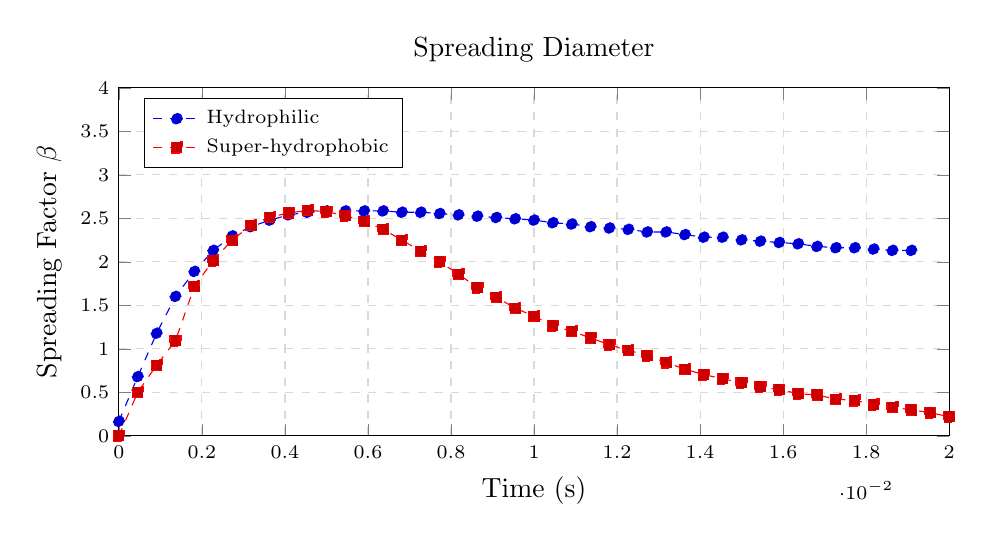
\begin{tikzpicture}
\begin{axis}[
	title = {Spreading Diameter},
    tick label style={font=\scriptsize},
    legend style={font=\scriptsize,/tikz/column 2/.style={column sep=5pt},},
    %legend columns=2,
    legend cell align=left,
	legend pos =north west,
    grid=major, % Display a grid
    grid style={dashed,gray!30}, % Set the style
    xlabel={Time (s)},
    ylabel={Spreading Factor $\beta$}, 
    ymin = 0, ymax = 4,
    ytick={0,0.5,...,4},
    %yticklabels={300,325,350,375,400,425,450,475,500,525},
    xmin = 0, xmax = 0.02,
    %ytick={0,1600,...,11200},
    %yticklabel style={
    %    /pgf/number format/fixed,
    %    /pgf/number format/precision=5},
	%scaled y ticks=false,
    width=1\textwidth, height=6cm,
    cycle list name= color
    ]
\addplot+[dashed]
coordinates {(	0	,	0.166303558	)
(	0.000454545	,	0.680332739	)
(	0.000909091	,	1.179243415	)
(	0.001363636	,	1.602561563	)
(	0.001818182	,	1.889813164	)
(	0.002272727	,	2.131709249	)
(	0.002727273	,	2.298012808	)
(	0.003181818	,	2.403842345	)
(	0.003636364	,	2.479434872	)
(	0.004090909	,	2.539908893	)
(	0.004545455	,	2.570145903	)
(	0.005	,	2.585264409	)
(	0.005454545	,	2.585264409	)
(	0.005909091	,	2.585264409	)
(	0.006363636	,	2.585264409	)
(	0.006818182	,	2.570145903	)
(	0.007272727	,	2.570145903	)
(	0.007727273	,	2.555027398	)
(	0.008181818	,	2.539908893	)
(	0.008636364	,	2.524790388	)
(	0.009090909	,	2.509671882	)
(	0.009545455	,	2.494553377	)
(	0.01	,	2.479434872	)
(	0.010454545	,	2.449197861	)
(	0.010909091	,	2.434079356	)
(	0.011363636	,	2.403842345	)
(	0.011818182	,	2.38872384	)
(	0.012272727	,	2.373605334	)
(	0.012727273	,	2.343368324	)
(	0.013181818	,	2.343368324	)
(	0.013636364	,	2.313131313	)
(	0.014090909	,	2.282894303	)
(	0.014545455	,	2.282894303	)
(	0.015	,	2.252657292	)
(	0.015454545	,	2.237538787	)
(	0.015909091	,	2.222420281	)
(	0.016363636	,	2.207301776	)
(	0.016818182	,	2.177064765	)
(	0.017272727	,	2.16194626	)
(	0.017727273	,	2.16194626	)
(	0.018181818	,	2.146827755	)
(	0.018636364	,	2.131709249	)
(	0.019090909	,	2.131709249	)
};
\addlegendentry{Hydrophilic}% $\theta_e=72.86º$}

\addplot+[dashed]
coordinates {(	0	,	0	)
(	0.000454545	,	0.499775013	)
(	0.000909091	,	0.812134396	)
(	0.001363636	,	1.093257841	)
(	0.001818182	,	1.717976608	)
(	0.002272727	,	2.014718022	)
(	0.002727273	,	2.248987559	)
(	0.003181818	,	2.42078522	)
(	0.003636364	,	2.514493035	)
(	0.004090909	,	2.561346942	)
(	0.004545455	,	2.592582881	)
(	0.005	,	2.576964912	)
(	0.005454545	,	2.530111004	)
(	0.005909091	,	2.467639127	)
(	0.006363636	,	2.373931312	)
(	0.006818182	,	2.248987559	)
(	0.007272727	,	2.124043806	)
(	0.007727273	,	1.999100053	)
(	0.008181818	,	1.85853833	)
(	0.008636364	,	1.702358639	)
(	0.009090909	,	1.593032854	)
(	0.009545455	,	1.468089101	)
(	0.01	,	1.374381286	)
(	0.010454545	,	1.265055502	)
(	0.010909091	,	1.202583625	)
(	0.011363636	,	1.12449378	)
(	0.011818182	,	1.046403934	)
(	0.012272727	,	0.983932057	)
(	0.012727273	,	0.92146018	)
(	0.013181818	,	0.843370335	)
(	0.013636364	,	0.765280489	)
(	0.014090909	,	0.702808612	)
(	0.014545455	,	0.655954705	)
(	0.015	,	0.609100797	)
(	0.015454545	,	0.56224689	)
(	0.015909091	,	0.531010951	)
(	0.016363636	,	0.484157044	)
(	0.016818182	,	0.468539075	)
(	0.017272727	,	0.421685167	)
(	0.017727273	,	0.406067198	)
(	0.018181818	,	0.359213291	)
(	0.018636364	,	0.327977352	)
(	0.019090909	,	0.296741414	)
(	0.019545455	,	0.265505476	)
(	0.02	,	0.218651568	)
(	0.020454545	,	0.171797661	)
(	0.020909091	,	0.124943753	)
(	0.021363636	,	0.062471877	)
(	0.021818182	,	0.062471877	)
};
\addlegendentry{Super-hydrophobic}% $\theta_e=22.39º$}
\end{axis}
\end{tikzpicture}
\caption{Spreading Factor along the radius for an Hydrophilic and Super-Hydrophobic}
\label{fig:shfdiameter}
\end{figure}

\begin{figure}[h!]
\centering
\subfigure[2 ms]{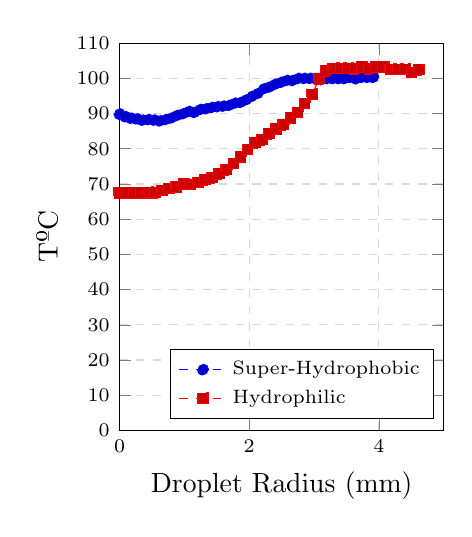
\begin{tikzpicture}
\begin{axis}[
	%title = {0.8 m/s || 13ms},
    tick label style={font=\scriptsize},
    legend style={font=\scriptsize,/tikz/column 2/.style={column sep=5pt},},
    %legend columns=2,
    legend cell align=left,
	legend pos =south east,
    grid=major, % Display a grid
    grid style={dashed,gray!30}, % Set the style
    xlabel={Droplet Radius (mm)},
    ylabel={TºC}, 
    ymin = 0, ymax = 110,
    ytick={0,10,...,110},
    %yticklabels={300,325,350,375,400,425,450,475,500,525},
    xmin = 0, xmax = 5,
    %ytick={0,1600,...,11200},
    %yticklabel style={
    %    /pgf/number format/fixed,
    %    /pgf/number format/precision=5},
	%scaled y ticks=false,
    width=0.47\textwidth, 
    height=6.5cm,
    cycle list name= color
    ]
\addplot+[dashed]
coordinates {(	0	,	89.86655059	)
(	0.089	,	89.10003191	)
(	0.178	,	88.65522678	)
(	0.267	,	88.46976353	)
(	0.356	,	88.10306248	)
(	0.445	,	88.2857149	)
(	0.534	,	88.13681502	)
(	0.623	,	87.90652516	)
(	0.712	,	88.28500619	)
(	0.801	,	88.74352291	)
(	0.89	,	89.46845453	)
(	0.979	,	89.92911366	)
(	1.068	,	90.59196773	)
(	1.157	,	90.32773089	)
(	1.246	,	91.14479336	)
(	1.335	,	91.35332748	)
(	1.424	,	91.71918634	)
(	1.513	,	91.93426697	)
(	1.602	,	92.09640908	)
(	1.691	,	92.31648637	)
(	1.78	,	92.93814861	)
(	1.869	,	93.16750821	)
(	1.958	,	93.91286337	)
(	2.047	,	94.90980271	)
(	2.136	,	95.71327372	)
(	2.225	,	97.02170984	)
(	2.314	,	97.53653533	)
(	2.403	,	98.3277948	)
(	2.492	,	98.8581068	)
(	2.581	,	99.4008084	)
(	2.67	,	99.38743867	)
(	2.759	,	99.96969898	)
(	2.848	,	99.96493866	)
(	2.937	,	99.96002977	)
(	3.026	,	99.9497384	)
(	3.115	,	99.62340733	)
(	3.204	,	99.93590686	)
(	3.293	,	99.93004602	)
(	3.382	,	99.92398349	)
(	3.471	,	99.91770899	)
(	3.56	,	100.2690377	)
(	3.649	,	99.86264706	)
(	3.738	,	100.2690377	)
(	3.827	,	100.2690377	)
(	3.916	,	100.2690377	)
};
\addlegendentry{Super-Hydrophobic}

\addplot+[dashed]
coordinates {(	0	,	67.43589175	)
(	0.11	,	67.43589175	)
(	0.22	,	67.43589175	)
(	0.33	,	67.43361264	)
(	0.44	,	67.57172905	)
(	0.55	,	67.57172905	)
(	0.66	,	68.2754645	)
(	0.77	,	68.83726786	)
(	0.88	,	69.13062977	)
(	0.99	,	69.99787327	)
(	1.1	,	69.88460648	)
(	1.21	,	70.51003936	)
(	1.32	,	71.25654954	)
(	1.43	,	71.75046404	)
(	1.54	,	72.93746386	)
(	1.65	,	74.05987972	)
(	1.76	,	75.86289984	)
(	1.87	,	77.6687978	)
(	1.98	,	79.87996387	)
(	2.09	,	81.69329754	)
(	2.2	,	82.56425241	)
(	2.31	,	84.26635378	)
(	2.42	,	85.61672194	)
(	2.53	,	86.75944654	)
(	2.64	,	88.73101821	)
(	2.75	,	90.36419265	)
(	2.86	,	92.93288303	)
(	2.97	,	95.47204255	)
(	3.08	,	99.86189818	)
(	3.19	,	102.0993129	)
(	3.3	,	102.8663733	)
(	3.41	,	102.8450046	)
(	3.52	,	102.8262885	)
(	3.63	,	102.7950717	)
(	3.74	,	103.269881	)
(	3.85	,	102.7463298	)
(	3.96	,	103.269881	)
(	4.07	,	103.269881	)
(	4.18	,	102.6432417	)
(	4.29	,	102.6033946	)
(	4.4	,	102.5584808	)
(	4.51	,	101.7370261	)
(	4.62	,	102.4491973	)
};
\addlegendentry{Hydrophilic}
\end{axis}
\end{tikzpicture}}
\subfigure[6 ms]{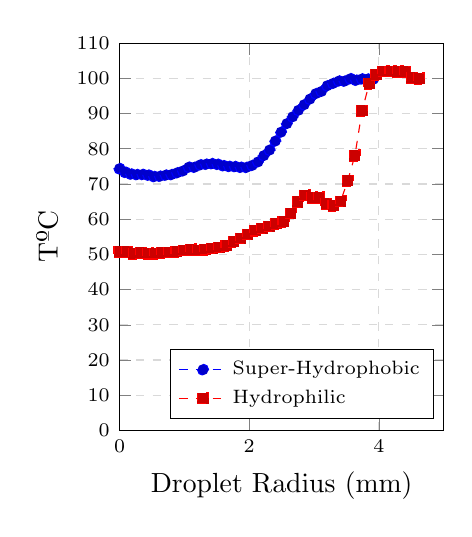
\begin{tikzpicture}
\begin{axis}[
	%title = {0.8 m/s || 13ms},
    tick label style={font=\scriptsize},
    legend style={font=\scriptsize,/tikz/column 2/.style={column sep=5pt},},
    %legend columns=2,
    legend cell align=left,
	legend pos =south east,
    grid=major, % Display a grid
    grid style={dashed,gray!30}, % Set the style
    xlabel={Droplet Radius (mm)},
    ylabel={TºC}, 
    ymin = 0, ymax = 110,
    ytick={0,10,...,110},
    %yticklabels={300,325,350,375,400,425,450,475,500,525},
    xmin = 0, xmax = 5,
    %ytick={0,1600,...,11200},
    %yticklabel style={
    %    /pgf/number format/fixed,
    %    /pgf/number format/precision=5},
	%scaled y ticks=false,
    width=0.47\textwidth, 
    height=6.5cm,
    cycle list name= color
    ]
\addplot+[dashed]
coordinates {(	0	,	74.34547995	)
(	0.089	,	73.30631541	)
(	0.178	,	72.80141687	)
(	0.267	,	72.64911917	)
(	0.356	,	72.69649396	)
(	0.445	,	72.49798311	)
(	0.534	,	72.09224396	)
(	0.623	,	72.19087526	)
(	0.712	,	72.50169265	)
(	0.801	,	72.65895303	)
(	0.89	,	73.18146962	)
(	0.979	,	73.70413247	)
(	1.068	,	74.75016474	)
(	1.157	,	74.75016474	)
(	1.246	,	75.42631983	)
(	1.335	,	75.59889097	)
(	1.424	,	75.76047215	)
(	1.513	,	75.56963827	)
(	1.602	,	75.17902778	)
(	1.691	,	74.97911094	)
(	1.78	,	74.93461485	)
(	1.869	,	74.72630405	)
(	1.958	,	74.70091693	)
(	2.047	,	75.27028586	)
(	2.136	,	76.26527188	)
(	2.225	,	78.05113915	)
(	2.314	,	79.63325601	)
(	2.403	,	82.18525281	)
(	2.492	,	84.72228578	)
(	2.581	,	87.14150264	)
(	2.67	,	89.0743903	)
(	2.759	,	90.9218155	)
(	2.848	,	92.51383787	)
(	2.937	,	94.11234522	)
(	3.026	,	95.6404885	)
(	3.115	,	96.28964647	)
(	3.204	,	97.8987052	)
(	3.293	,	98.55533851	)
(	3.382	,	99.22811344	)
(	3.471	,	99.20909094	)
(	3.56	,	99.89025974	)
(	3.649	,	99.4536595	)
(	3.738	,	99.82096395	)
(	3.827	,	99.78247992	)
(	3.916	,	99.73006389	)
};
\addlegendentry{Super-Hydrophobic}

\addplot+[dashed]
coordinates {(	0	,	50.78401418	)
(	0.11	,	50.78401418	)
(	0.22	,	50.17772058	)
(	0.33	,	50.48235049	)
(	0.44	,	50.27473108	)
(	0.55	,	50.27473108	)
(	0.66	,	50.48539209	)
(	0.77	,	50.59194523	)
(	0.88	,	50.80755155	)
(	0.99	,	51.13738169	)
(	1.1	,	51.36168668	)
(	1.21	,	51.16734408	)
(	1.32	,	51.39993808	)
(	1.43	,	51.75621655	)
(	1.54	,	51.99882917	)
(	1.65	,	52.49682959	)
(	1.76	,	53.55794154	)
(	1.87	,	54.62906905	)
(	1.98	,	55.71127842	)
(	2.09	,	56.80567395	)
(	2.2	,	57.41129497	)
(	2.31	,	58.04114283	)
(	2.42	,	58.69691121	)
(	2.53	,	59.20686183	)
(	2.64	,	61.64778158	)
(	2.75	,	64.8755955	)
(	2.86	,	66.79186139	)
(	2.97	,	66.13488894	)
(	3.08	,	66.13398152	)
(	3.19	,	64.39060772	)
(	3.3	,	63.8084878	)
(	3.41	,	65.09634021	)
(	3.52	,	70.95043645	)
(	3.63	,	78.06385095	)
(	3.74	,	90.73531804	)
(	3.85	,	98.40435158	)
(	3.96	,	101.00536	)
(	4.07	,	102.0654551	)
(	4.18	,	102.0109297	)
(	4.29	,	101.9305602	)
(	4.4	,	101.8399335	)
(	4.51	,	100.1709287	)
(	4.62	,	99.93059749	)
};
\addlegendentry{Hydrophilic}
\end{axis}
\end{tikzpicture}}
\subfigure[12 ms]{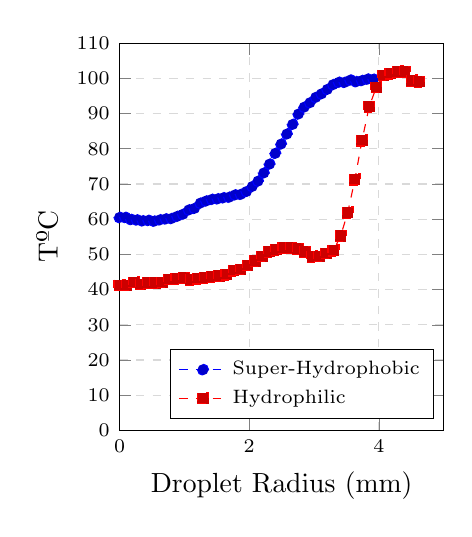
\begin{tikzpicture}
\begin{axis}[
	%title = {0.8 m/s || 13ms},
    tick label style={font=\scriptsize},
    legend style={font=\scriptsize,/tikz/column 2/.style={column sep=5pt},},
    %legend columns=2,
    legend cell align=left,
	legend pos =south east,
    grid=major, % Display a grid
    grid style={dashed,gray!30}, % Set the style
    xlabel={Droplet Radius (mm)},
    ylabel={TºC}, 
    ymin = 0, ymax = 110,
    ytick={0,10,...,110},
    %yticklabels={300,325,350,375,400,425,450,475,500,525},
    xmin = 0, xmax = 5,
    %ytick={0,1600,...,11200},
    %yticklabel style={
    %    /pgf/number format/fixed,
    %    /pgf/number format/precision=5},
	%scaled y ticks=false,
    width=0.47\textwidth, 
    height=6.5cm,
    cycle list name= color
    ]
\addplot+[dashed]
coordinates {(	0	,	60.48825861	)
(	0.089	,	60.48825861	)
(	0.178	,	59.89600924	)
(	0.267	,	59.77070914	)
(	0.356	,	59.52296368	)
(	0.445	,	59.64636477	)
(	0.534	,	59.42594377	)
(	0.623	,	59.80471019	)
(	0.712	,	60.06219901	)
(	0.801	,	60.19247741	)
(	0.89	,	60.8009647	)
(	0.979	,	61.40744916	)
(	1.068	,	62.61494631	)
(	1.157	,	63.07533593	)
(	1.246	,	64.56091952	)
(	1.335	,	65.16036182	)
(	1.424	,	65.61418062	)
(	1.513	,	65.76804526	)
(	1.602	,	66.07977706	)
(	1.691	,	66.23768396	)
(	1.78	,	66.8834014	)
(	1.869	,	67.04846117	)
(	1.958	,	67.84566919	)
(	2.047	,	69.28160173	)
(	2.136	,	70.80923928	)
(	2.225	,	73.1209793	)
(	2.314	,	75.63296917	)
(	2.403	,	78.70342514	)
(	2.492	,	81.33469094	)
(	2.581	,	84.18832843	)
(	2.67	,	86.91838732	)
(	2.759	,	89.86450918	)
(	2.848	,	91.81955283	)
(	2.937	,	93.07982637	)
(	3.026	,	94.60102868	)
(	3.115	,	95.60043054	)
(	3.204	,	96.85428244	)
(	3.293	,	98.20684929	)
(	3.382	,	98.8772453	)
(	3.471	,	98.85174668	)
(	3.56	,	99.50920442	)
(	3.649	,	99.0420348	)
(	3.738	,	99.36977711	)
(	3.827	,	99.78247992	)
(	3.916	,	99.73006389	)
};
\addlegendentry{Super-Hydrophobic}

\addplot+[dashed]
coordinates {(	0	,	41.28542872	)
(	0.11	,	41.28542872	)
(	0.22	,	42.04915906	)
(	0.33	,	41.53607336	)
(	0.44	,	41.87913443	)
(	0.55	,	41.87913443	)
(	0.66	,	42.05461624	)
(	0.77	,	42.92297692	)
(	0.88	,	43.1059006	)
(	0.99	,	43.38573352	)
(	1.1	,	42.78457458	)
(	1.21	,	43.16747549	)
(	1.32	,	43.36370408	)
(	1.43	,	43.66427942	)
(	1.54	,	43.86896025	)
(	1.65	,	44.28909973	)
(	1.76	,	45.43937336	)
(	1.87	,	45.7794094	)
(	1.98	,	46.94973098	)
(	2.09	,	48.12642448	)
(	2.2	,	49.44318808	)
(	2.31	,	50.78284617	)
(	2.42	,	51.35660787	)
(	2.53	,	51.80278695	)
(	2.64	,	51.91127184	)
(	2.75	,	51.54381096	)
(	2.86	,	50.75849083	)
(	2.97	,	49.38710743	)
(	3.08	,	49.4351773	)
(	3.19	,	50.34726218	)
(	3.3	,	51.12224953	)
(	3.41	,	55.22872654	)
(	3.52	,	61.87841963	)
(	3.63	,	71.28108158	)
(	3.74	,	82.36911281	)
(	3.85	,	91.92402779	)
(	3.96	,	97.45982021	)
(	4.07	,	100.8396544	)
(	4.18	,	101.3728217	)
(	4.29	,	101.9305602	)
(	4.4	,	101.8399335	)
(	4.51	,	99.37487226	)
(	4.62	,	99.0713457	)
};
\addlegendentry{Hydrophilic}
\end{axis}
\end{tikzpicture}}
\subfigure[24 ms]{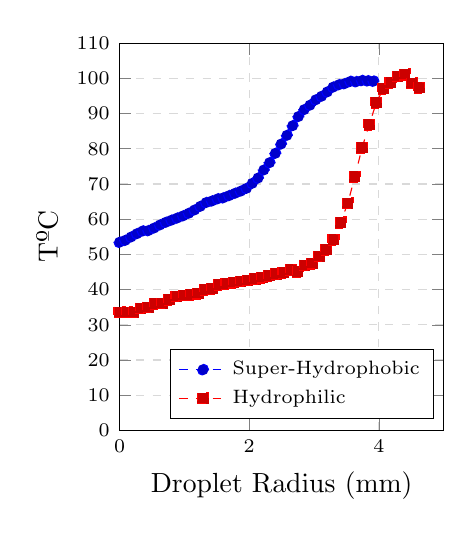
\begin{tikzpicture}
\begin{axis}[
	%title = {0.8 m/s || 13ms},
    tick label style={font=\scriptsize},
    legend style={font=\scriptsize,/tikz/column 2/.style={column sep=5pt},},
    %legend columns=2,
    legend cell align=left,
	legend pos =south east,
    grid=major, % Display a grid
    grid style={dashed,gray!30}, % Set the style
    xlabel={Droplet Radius (mm)},
    ylabel={TºC}, 
    ymin = 0, ymax = 110,
    ytick={0,10,...,110},
    %yticklabels={300,325,350,375,400,425,450,475,500,525},
    xmin = 0, xmax = 5,
    %ytick={0,1600,...,11200},
    %yticklabel style={
    %    /pgf/number format/fixed,
    %    /pgf/number format/precision=5},
	%scaled y ticks=false,
    width=0.47\textwidth, 
    height=6.5cm,
    cycle list name= color
    ]
\addplot+[dashed]
coordinates {(	0	,	53.44836384	)
(	0.089	,	53.99245765	)
(	0.178	,	54.94371683	)
(	0.267	,	55.86474942	)
(	0.356	,	56.63985306	)
(	0.445	,	56.75727697	)
(	0.534	,	57.49231159	)
(	0.623	,	58.35358751	)
(	0.712	,	59.09610635	)
(	0.801	,	59.71108478	)
(	0.89	,	60.32379712	)
(	0.979	,	60.93438715	)
(	1.068	,	61.67964207	)
(	1.157	,	62.61494631	)
(	1.246	,	63.64588596	)
(	1.335	,	64.70863125	)
(	1.424	,	65.15930391	)
(	1.513	,	65.76804526	)
(	1.602	,	66.07977706	)
(	1.691	,	66.69239517	)
(	1.78	,	67.34254535	)
(	1.869	,	67.96457582	)
(	1.958	,	68.75753315	)
(	2.047	,	70.18322471	)
(	2.136	,	71.6887036	)
(	2.225	,	73.97678964	)
(	2.314	,	76.04728949	)
(	2.403	,	78.70342514	)
(	2.492	,	81.33469094	)
(	2.581	,	83.80780049	)
(	2.67	,	86.55087398	)
(	2.759	,	89.14865789	)
(	2.848	,	91.11689349	)
(	2.937	,	92.38129378	)
(	3.026	,	93.89788534	)
(	3.115	,	94.90324096	)
(	3.204	,	96.14794884	)
(	3.293	,	97.50391053	)
(	3.382	,	98.16950802	)
(	3.471	,	98.49234138	)
(	3.56	,	99.12583842	)
(	3.649	,	99.0420348	)
(	3.738	,	99.36977711	)
(	3.827	,	99.29229726	)
(	3.916	,	99.18671524	)
};
\addlegendentry{Super-Hydrophobic}

\addplot+[dashed]
coordinates {(	0	,	33.56004002	)
(	0.11	,	33.56004002	)
(	0.22	,	33.56004002	)
(	0.33	,	34.71744217	)
(	0.44	,	35.00418577	)
(	0.55	,	35.93977223	)
(	0.66	,	36.09036695	)
(	0.77	,	37.08351396	)
(	0.88	,	38.13927195	)
(	0.99	,	38.38686273	)
(	1.1	,	38.55523984	)
(	1.21	,	38.90029029	)
(	1.32	,	39.97454	)
(	1.43	,	40.25162337	)
(	1.54	,	41.32679706	)
(	1.65	,	41.72258986	)
(	1.76	,	42.02872584	)
(	1.87	,	42.34323902	)
(	1.98	,	42.66652799	)
(	2.09	,	42.9990183	)
(	2.2	,	43.45744274	)
(	2.31	,	43.93420567	)
(	2.42	,	44.43058913	)
(	2.53	,	44.81659592	)
(	2.64	,	45.62673264	)
(	2.75	,	45.06445936	)
(	2.86	,	46.94859408	)
(	2.97	,	47.42113366	)
(	3.08	,	49.4351773	)
(	3.19	,	51.35803055	)
(	3.3	,	54.13609294	)
(	3.41	,	59.04636662	)
(	3.52	,	64.51209533	)
(	3.63	,	72.07652719	)
(	3.74	,	80.26203593	)
(	3.85	,	86.76036346	)
(	3.96	,	93.06893351	)
(	4.07	,	97.02446374	)
(	4.18	,	98.7598137	)
(	4.29	,	100.5652629	)
(	4.4	,	101.114067	)
(	4.51	,	98.56983716	)
(	4.62	,	97.32157794	)
};
\addlegendentry{Hydrophilic}
\end{axis}
\end{tikzpicture}}
\caption{Temperature along the radius for Ethanol and Water}
\label{fig:shftemp}
\end{figure}

\par Looking now at the temperature field for the initial temperature of 100ºC, depicted in Figure \ref{fig:shftemp}, one can better draw conclusions about heat transfer phenomena. It is clear from the figure, that the droplet impacting on the super-hydrophobic surface removes less heat, as both the temperature drop and spreading diameter are smaller in the super-hydrophobic surface case. In the center of the droplet, a large slope is nonetheless observable in the center in the super-hydrophobic surface. This is caused by the way the droplet leaves the surface, as all liquid is concentrated in a small radius. Note that the wetted area radius is also smaller. There is no apparent temperature effect of the formed lamella rim, and some unusual curves appear near the droplet center. These phenomena can only be analyzed with the help of the images that one can obtain from the developed code. These images are shown in Figure \ref{fig:shftemp}. In the 6ms panel one can barely see the rim, but it's still visible. The colormap for these images was shortened in order to improve the contrast, or else the lamella's rim wouldn't be visible at all. There are also some unusual spots in the image. The cause of this is the fact that, after some tests the foil's coating gets uneven and the droplet shape is affected. In the first tests this didn't happen, and the shape was more uniform. The IR Images for the first experiment can be seen in Figure \ref{fig:shfim2}. This means that the foil requires a new coating after some tests. The results for the initial temperature of 100ºC are not invalidated but have should have a slightly higher heat flux than normal. The heat flux is slightly higher than expected which may be due to the aging of the surface coating \\

\begin{figure}[h!]
\centering
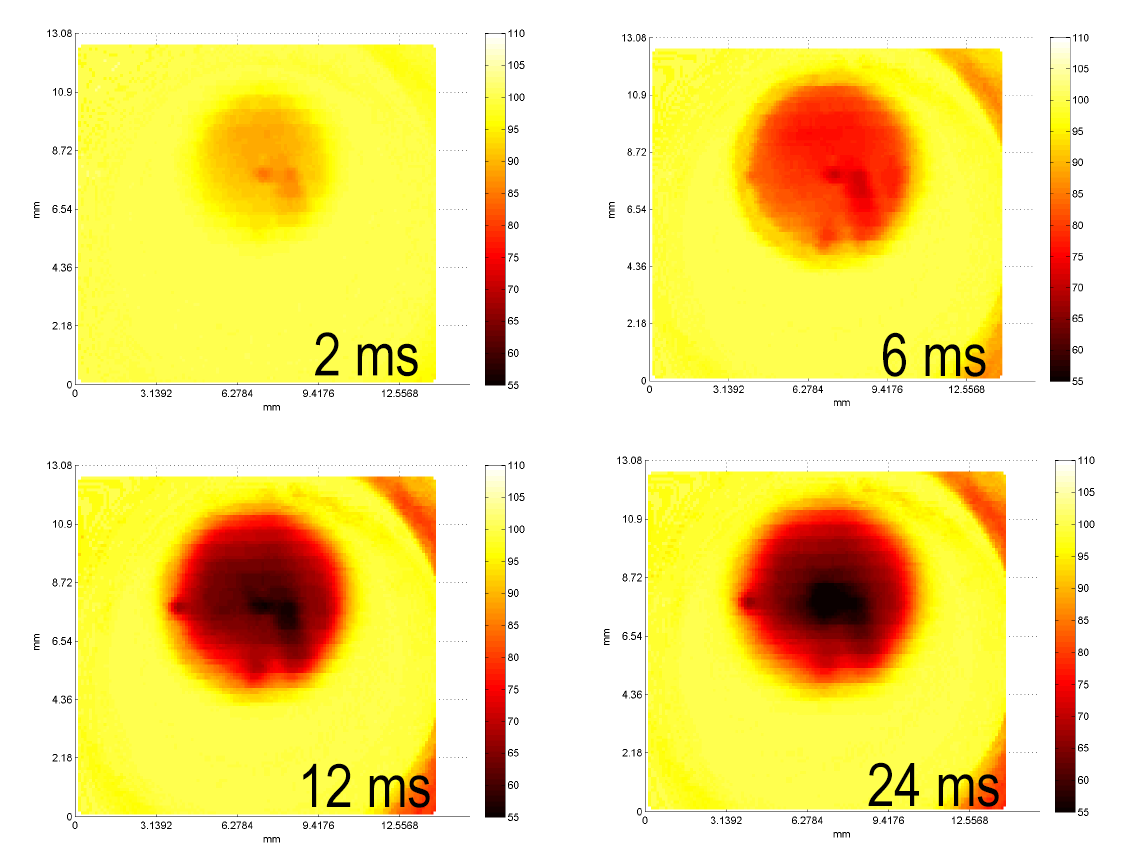
\includegraphics[height=0.45\textheight]{Figures/5.Chapter/shfim.png}
\caption{IR Images for a Super-Hydrophobic surface droplet impact at 0.8 m/s impact speed (foil initial temperature at 100ºC)}
\label{fig:shfim}
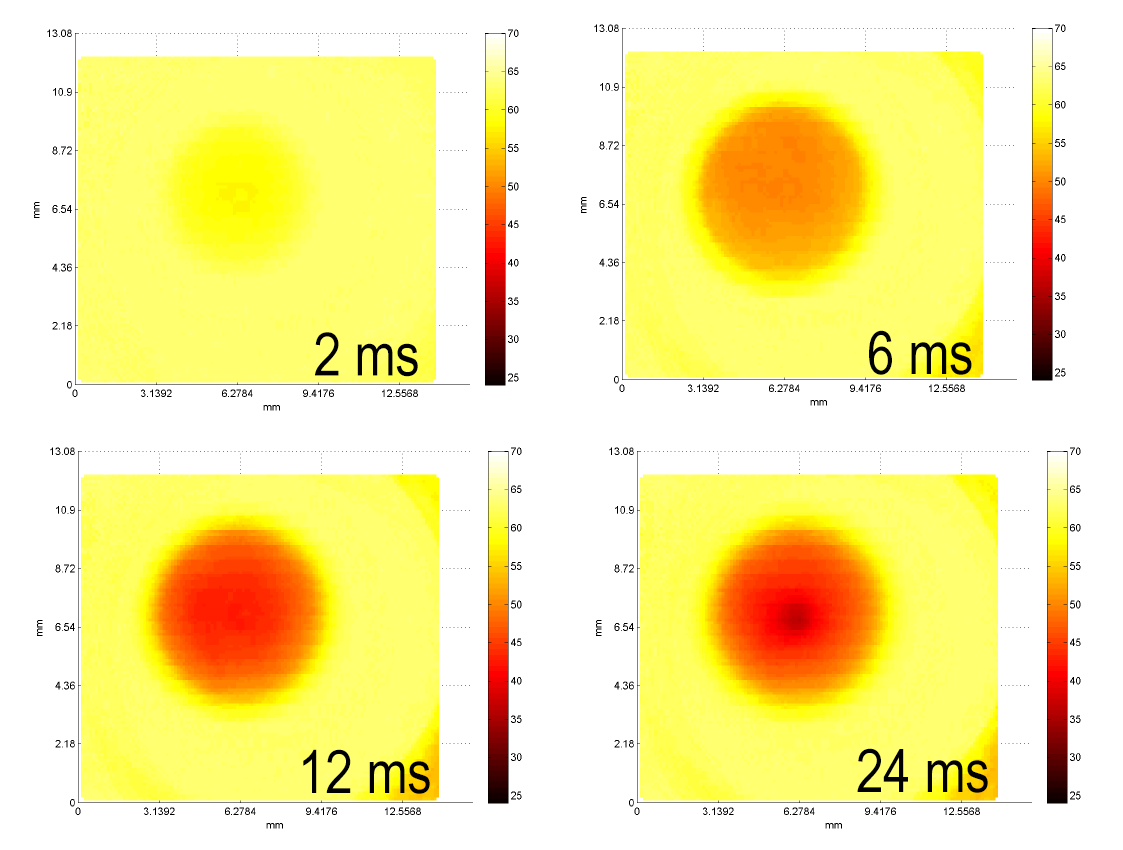
\includegraphics[height=0.45\textheight]{Figures/5.Chapter/shfim2.png}
\caption{IR Images for a Super-Hydrophobic surface droplet impact at 0.8 m/s impact speed (foil initial temperature at 100ºC)}
\label{fig:shfim2}
\end{figure}

\par Moving on to the heat flux plots, depicted in Figure \ref{fig:shfflux}. The heat flux is considerably smaller for the super-hydrophobic surface. The heat flux peaks at the contact edge are also smaller. This is representative of a high contact angle as the liquid in the edge is above the surface but not touching it. There is a small peak in the 4 ms plot that's caused by the fact that the droplet is reaching maximum diameter as stated before. This peak is still relatively smaller to the center heat flux in the super-hydrophobic surface test. The flux at the center is very similar between both cases in this same timestep. The cause of this is related to the thickness of the droplet. The thickness is higher in the studied case, so it's expected to remove more heat. This heat flux, as stated before is also expected to be a bit higher than expected. What can also be seen is the apparently smaller diameter. This is explained by the high contact angle, as stated before.\\

\begin{figure}[h]
\centering
\subfigure[2 ms]{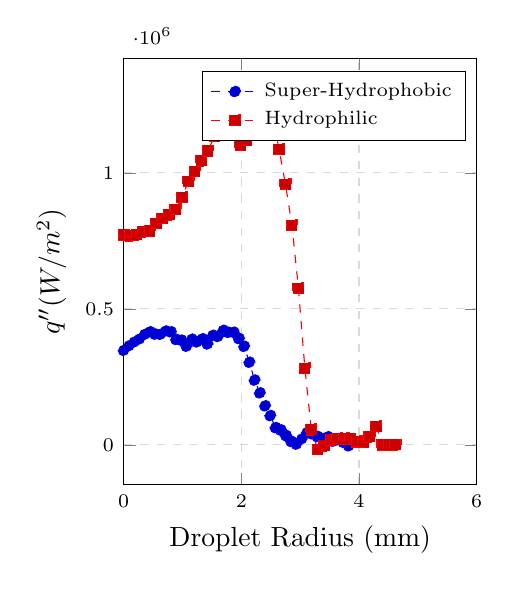
\begin{tikzpicture}
\begin{axis}[
	%title = {107 ºC || $T_{amb}=24$},
    tick label style={font=\scriptsize},
    legend style={font=\scriptsize,/tikz/column 2/.style={column sep=5pt},},
    %legend columns=2,
    legend cell align=left,
	legend pos =north east,
    grid=major, % Display a grid
    grid style={dashed,gray!30}, % Set the style
    xlabel={Droplet Radius (mm)},
    ylabel={$q''(W/m^2)$}, 
    %ymin = 55, ymax = 113,
    %ytick={60,70,...,100,110},
    %yticklabels={300,325,350,375,400,425,450,475,500,525},
    xmin = 0, xmax = 6,
    %ytick={0,1600,...,11200},
    %yticklabel style={
    %    /pgf/number format/fixed,
    %    /pgf/number format/precision=5},
	%scaled y ticks=false,
    width=0.5\textwidth, height=7cm,
    cycle list name= color
    ]
\addplot+[dashed]
coordinates {(	0	,	347691.7121	)
(	0.089	,	364260.5561	)
(	0.178	,	378129.5961	)
(	0.267	,	389108.8051	)
(	0.356	,	406260.9391	)
(	0.445	,	415726.5627	)
(	0.534	,	407043.0824	)
(	0.623	,	406427.966	)
(	0.712	,	418477.5697	)
(	0.801	,	415450.0438	)
(	0.89	,	387642.7827	)
(	0.979	,	384917.4299	)
(	1.068	,	362567.5929	)
(	1.157	,	388432.0543	)
(	1.246	,	378303.9002	)
(	1.335	,	390093.3924	)
(	1.424	,	370844.2725	)
(	1.513	,	402663.1833	)
(	1.602	,	398424.1921	)
(	1.691	,	421025.4037	)
(	1.78	,	413460.1326	)
(	1.869	,	413956.6838	)
(	1.958	,	390919.2973	)
(	2.047	,	362046.6662	)
(	2.136	,	303657.1802	)
(	2.225	,	238022.3595	)
(	2.314	,	190968.7385	)
(	2.403	,	143460.9892	)
(	2.492	,	107588.7748	)
(	2.581	,	63446.45228	)
(	2.67	,	54683.21562	)
(	2.759	,	34132.79707	)
(	2.848	,	12536.64249	)
(	2.937	,	2603.149999	)
(	3.026	,	21893.80769	)
(	3.115	,	45288.81367	)
(	3.204	,	40447.52217	)
(	3.293	,	30537.16188	)
(	3.382	,	22342.88731	)
(	3.471	,	29623.41028	)
(	3.56	,	13172.5573	)
(	3.649	,	18617.6588	)
(	3.738	,	9600.975032	)
(	3.827	,	-3637.921028	)
};
\addlegendentry{Super-Hydrophobic}

\addplot+[dashed]
coordinates {(	0	,	771569.1555	)
(	0.11	,	768629.0196	)
(	0.22	,	772011.5775	)
(	0.33	,	783637.3806	)
(	0.44	,	786386.6358	)
(	0.55	,	814650.0075	)
(	0.66	,	833259.4286	)
(	0.77	,	846535.1734	)
(	0.88	,	866118.4552	)
(	0.99	,	910386.7527	)
(	1.1	,	968920.2045	)
(	1.21	,	1005681.021	)
(	1.32	,	1044742.093	)
(	1.43	,	1080449.949	)
(	1.54	,	1134309.662	)
(	1.65	,	1181742.021	)
(	1.76	,	1183180.613	)
(	1.87	,	1153428.011	)
(	1.98	,	1101940.083	)
(	2.09	,	1120779.629	)
(	2.2	,	1195808.773	)
(	2.31	,	1282731.153	)
(	2.42	,	1290623.843	)
(	2.53	,	1210554.62	)
(	2.64	,	1087505.867	)
(	2.75	,	958009.4697	)
(	2.86	,	807772.709	)
(	2.97	,	576056.5252	)
(	3.08	,	281680.1447	)
(	3.19	,	56273.1891	)
(	3.3	,	-16746.90567	)
(	3.41	,	-2584.392404	)
(	3.52	,	17864.27049	)
(	3.63	,	23738.61687	)
(	3.74	,	23004.11932	)
(	3.85	,	21788.02636	)
(	3.96	,	12319.07671	)
(	4.07	,	9203.863393	)
(	4.18	,	29514.02343	)
(	4.29	,	67819.7116	)
(	4.4	,	101.114067	)
(	4.51	,	98.56983716	)
(	4.62	,	97.32157794	)
};
\addlegendentry{Hydrophilic}
\end{axis}
\end{tikzpicture}}
\subfigure[4 ms]{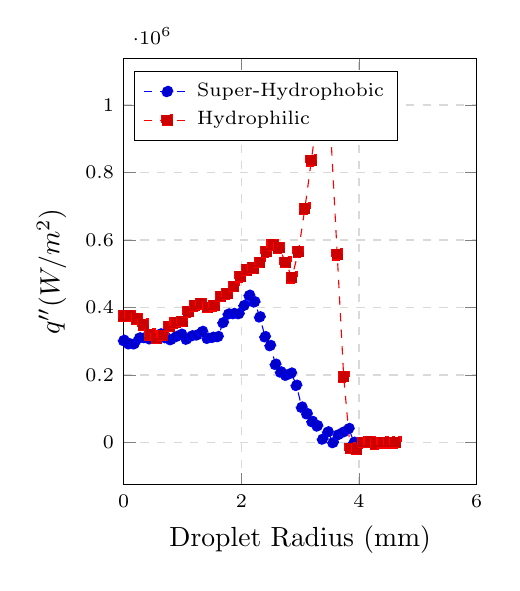
\begin{tikzpicture}
\begin{axis}[
	%title = {107 ºC || $T_{amb}=24$},
    tick label style={font=\scriptsize},
    legend style={font=\scriptsize,/tikz/column 2/.style={column sep=5pt},},
    %legend columns=2,
    legend cell align=left,
	legend pos =north west,
    grid=major, % Display a grid
    grid style={dashed,gray!30}, % Set the style
    xlabel={Droplet Radius (mm)},
    ylabel={$q''(W/m^2)$}, 
    %ymin = 55, ymax = 113,
    %ytick={60,70,...,100,110},
    %yticklabels={300,325,350,375,400,425,450,475,500,525},
    xmin = 0, xmax = 6,
    %ytick={0,1600,...,11200},
    %yticklabel style={
    %    /pgf/number format/fixed,
    %    /pgf/number format/precision=5},
	%scaled y ticks=false,
    width=0.5\textwidth, height=7cm,
    cycle list name= color
    ]
\addplot+[dashed]
coordinates {(	0	,	302498.0315	)
(	0.089	,	292370.6108	)
(	0.178	,	292176.6277	)
(	0.267	,	309675.955	)
(	0.356	,	310695.9516	)
(	0.445	,	307224.3009	)
(	0.534	,	315243.3713	)
(	0.623	,	321519.1342	)
(	0.712	,	310568.7037	)
(	0.801	,	304613.8845	)
(	0.89	,	313485.552	)
(	0.979	,	320471.3586	)
(	1.068	,	305953.7542	)
(	1.157	,	315784.2418	)
(	1.246	,	318517.2978	)
(	1.335	,	328838.32	)
(	1.424	,	308661.5312	)
(	1.513	,	311397.4074	)
(	1.602	,	313645.2767	)
(	1.691	,	355177.9159	)
(	1.78	,	380591.9929	)
(	1.869	,	381832.7638	)
(	1.958	,	381565.8679	)
(	2.047	,	405906.1794	)
(	2.136	,	435993.8851	)
(	2.225	,	416346.3819	)
(	2.314	,	371971.32	)
(	2.403	,	313202.0362	)
(	2.492	,	286956.0089	)
(	2.581	,	231618.5191	)
(	2.67	,	208715.8026	)
(	2.759	,	199170.9759	)
(	2.848	,	205390.1858	)
(	2.937	,	169191.2314	)
(	3.026	,	104593.7752	)
(	3.115	,	85106.57231	)
(	3.204	,	62042.80446	)
(	3.293	,	48847.81135	)
(	3.382	,	10031.16414	)
(	3.471	,	31165.14813	)
(	3.56	,	-371.5349289	)
(	3.649	,	22987.35159	)
(	3.738	,	30964.96886	)
(	3.827	,	41062.35688	)
(	3.916	,	99.18671524	)
};
\addlegendentry{Super-Hydrophobic}

\addplot+[dashed]
coordinates {(	0	,	375855.571	)
(	0.11	,	374865.716	)
(	0.22	,	366399.9126	)
(	0.33	,	349323.4841	)
(	0.44	,	319834.6935	)
(	0.55	,	308976.9931	)
(	0.66	,	317592.7393	)
(	0.77	,	343871.0505	)
(	0.88	,	354573.6172	)
(	0.99	,	358941.4379	)
(	1.1	,	387366.2033	)
(	1.21	,	405519.4485	)
(	1.32	,	411189.6223	)
(	1.43	,	400352.1419	)
(	1.54	,	405927.3853	)
(	1.65	,	432835.7083	)
(	1.76	,	440262.1351	)
(	1.87	,	463151.759	)
(	1.98	,	491905.7223	)
(	2.09	,	510989.816	)
(	2.2	,	516928.2872	)
(	2.31	,	534295.7526	)
(	2.42	,	565322.7071	)
(	2.53	,	585581.9192	)
(	2.64	,	577130.6179	)
(	2.75	,	534490.7369	)
(	2.86	,	488978.4408	)
(	2.97	,	565482.5437	)
(	3.08	,	693160.8652	)
(	3.19	,	835734.1971	)
(	3.3	,	980738.2935	)
(	3.41	,	1033011.115	)
(	3.52	,	917184.6882	)
(	3.63	,	557060.0077	)
(	3.74	,	194637.235	)
(	3.85	,	-17313.51997	)
(	3.96	,	-20522.37192	)
(	4.07	,	191.9630829	)
(	4.18	,	1782.560803	)
(	4.29	,	-4264.146327	)
(	4.4	,	101.114067	)
(	4.51	,	98.56983716	)
(	4.62	,	97.32157794	)
};
\addlegendentry{Hydrophilic}
\end{axis}
\end{tikzpicture}}
\caption{Heat Flux comparison along the radius for a droplet impact in surfaces with different wettability}
\label{fig:shfflux}
\end{figure}

\par The cooling effectiveness will describe what kind of surface is easier to cool with droplets. The comparison between both surfaces is shown in Figure \ref{fig:shfcool}. This parameter shows considerably lower values for the super-hydrophobic surface. After some timesteps, the cooling effectiveness stabilizes. This occurs because the droplet leaves the surface. From that point on there is no more heat removal, while in the hydrophilic surface, the droplet continues to remove heat. Hence the bad cooling performance obtained when using a super hydrophobic surface is not just caused by the reduced wetting area, but also due to the smaller time interval in which the droplet contacts the surface.

\begin{figure}[h]
\centering
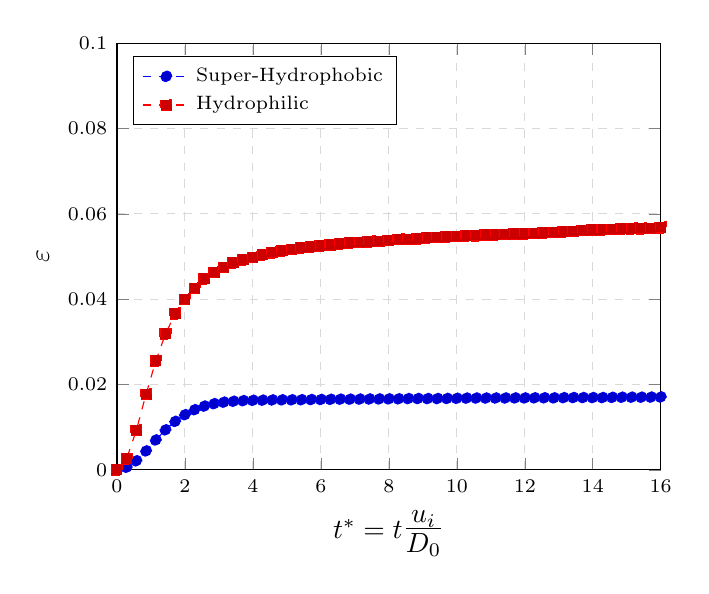
\begin{tikzpicture}
\begin{axis}[
	%title = {$20 ºC || $T_{amb}=24$},
    tick label style={font=\scriptsize},
    legend style={font=\scriptsize,/tikz/column 2/.style={column sep=5pt},},
    %legend columns=2,
    legend cell align=left,
	legend pos =north west,
    grid=major, % Display a grid
    grid style={dashed,gray!30}, % Set the style
    xlabel={$t^*=t$\Large{$\frac{u_i}{D_0}$}},
    ylabel={$\varepsilon$}, 
    ymin = 0, ymax = 0.1,
    ytick={0,0.02,0.04,0.06,0.08,0.1},
    yticklabels={0,0.02,0.04,0.06,0.08,0.1},
    xmin = 0, xmax = 16,
    %ytick={0,1600,...,11200},
    %yticklabel style={
    %    /pgf/number format/fixed,
    %    /pgf/number format/precision=5},
	%scaled y ticks=false,
    width=0.7\textwidth, 
    height=7cm,
    cycle list name= color
    ]
\addplot+[dashed]
coordinates {(	0	,	0	)
(	0.285714286	,	0.000591316	)
(	0.571428571	,	0.002106067	)
(	0.857142857	,	0.004416029	)
(	1.142857143	,	0.006987625	)
(	1.428571429	,	0.009360968	)
(	1.714285714	,	0.011347245	)
(	2	,	0.012907333	)
(	2.285714286	,	0.014079235	)
(	2.571428571	,	0.014924092	)
(	2.857142857	,	0.015492375	)
(	3.142857143	,	0.015845785	)
(	3.428571429	,	0.016055844	)
(	3.714285714	,	0.016199658	)
(	4	,	0.016274981	)
(	4.285714286	,	0.016311294	)
(	4.571428571	,	0.016366868	)
(	4.857142857	,	0.016392865	)
(	5.142857143	,	0.016396488	)
(	5.428571429	,	0.016418383	)
(	5.714285714	,	0.016456926	)
(	6	,	0.016476686	)
(	6.285714286	,	0.016510127	)
(	6.571428571	,	0.016543789	)
(	6.857142857	,	0.016546657	)
(	7.142857143	,	0.01656801	)
(	7.428571429	,	0.01659141	)
(	7.714285714	,	0.016602012	)
(	8	,	0.016616232	)
(	8.285714286	,	0.016634548	)
(	8.571428571	,	0.016681335	)
(	8.857142857	,	0.016700159	)
(	9.142857143	,	0.016691175	)
(	9.428571429	,	0.016694709	)
(	9.714285714	,	0.016714517	)
(	10	,	0.016752256	)
(	10.28571429	,	0.016796484	)
(	10.57142857	,	0.016812974	)
(	10.85714286	,	0.016811627	)
(	11.14285714	,	0.016822666	)
(	11.42857143	,	0.016827844	)
(	11.71428571	,	0.016840528	)
(	12	,	0.016837973	)
(	12.28571429	,	0.016862388	)
(	12.57142857	,	0.01686967	)
(	12.85714286	,	0.016854412	)
(	13.14285714	,	0.016902121	)
(	13.42857143	,	0.01692745	)
(	13.71428571	,	0.016926109	)
(	14	,	0.016920104	)
(	14.28571429	,	0.016923112	)
(	14.57142857	,	0.016971015	)
(	14.85714286	,	0.016997868	)
(	15.14285714	,	0.017007495	)
(	15.42857143	,	0.017008957	)
(	15.71428571	,	0.017031054	)
(	16	,	0.017060046	)
(	16.28571429	,	0.017055986	)
(	16.57142857	,	0.017068733	)
(	16.85714286	,	0	)
};
\addlegendentry{Super-Hydrophobic}
\addplot+[dashed]
coordinates {(	0	,	0	)
(	0.285714286	,	0.002612585	)
(	0.571428571	,	0.009302215	)
(	0.857142857	,	0.017749228	)
(	1.142857143	,	0.025515761	)
(	1.428571429	,	0.031850811	)
(	1.714285714	,	0.036612861	)
(	2	,	0.040000188	)
(	2.285714286	,	0.042584131	)
(	2.571428571	,	0.044725349	)
(	2.857142857	,	0.046299304	)
(	3.142857143	,	0.047513768	)
(	3.428571429	,	0.048503244	)
(	3.714285714	,	0.049224205	)
(	4	,	0.049822113	)
(	4.285714286	,	0.050384046	)
(	4.571428571	,	0.050945747	)
(	4.857142857	,	0.051366275	)
(	5.142857143	,	0.051667129	)
(	5.428571429	,	0.051998352	)
(	5.714285714	,	0.052328076	)
(	6	,	0.052478495	)
(	6.285714286	,	0.052679505	)
(	6.571428571	,	0.052992206	)
(	6.857142857	,	0.053194257	)
(	7.142857143	,	0.053349955	)
(	7.428571429	,	0.05349325	)
(	7.714285714	,	0.053608407	)
(	8	,	0.05383981	)
(	8.285714286	,	0.053995906	)
(	8.571428571	,	0.054063631	)
(	8.857142857	,	0.05419384	)
(	9.142857143	,	0.05437016	)
(	9.428571429	,	0.054541661	)
(	9.714285714	,	0.054617238	)
(	10	,	0.054741438	)
(	10.28571429	,	0.054849401	)
(	10.57142857	,	0.05492757	)
(	10.85714286	,	0.055033164	)
(	11.14285714	,	0.055117619	)
(	11.42857143	,	0.055192166	)
(	11.71428571	,	0.055266081	)
(	12	,	0.055333218	)
(	12.28571429	,	0.055444001	)
(	12.57142857	,	0.055589794	)
(	12.85714286	,	0.055702094	)
(	13.14285714	,	0.055821021	)
(	13.42857143	,	0.0559515	)
(	13.71428571	,	0.056120152	)
(	14	,	0.056208202	)
(	14.28571429	,	0.05624163	)
(	14.57142857	,	0.056380573	)
(	14.85714286	,	0.056487899	)
(	15.14285714	,	0.056534491	)
(	15.42857143	,	0.056562845	)
(	15.71428571	,	0.05663789	)
(	16	,	0.056799011	)
(	16.28571429	,	0.056875806	)
(	16.57142857	,	0.056934081	)
(	16.85714286	,	0	)
};
\addlegendentry{Hydrophilic}
\end{axis}
\end{tikzpicture}
\caption{Cooling Effectiveness comparison along the radius for a droplet impact in surfaces with different wettability}
\label{fig:shfcool}
\end{figure}